\documentclass[12pt]{article}
\usepackage[utf8]{inputenc}
\usepackage{preamble}

\begin{document}


%%%%%%%%%%%%%%%%%%%%%%%%%%%%%%%%%%%%%%%%%%%%%%%%%%%%%
%%%%%%%%%%%%%%%%%%%%% Portada %%%%%%%%%%%%%%%%%%%%%%%
%%%%%%%%%%%%%%%%%%%%%%%%%%%%%%%%%%%%%%%%%%%%%%%%%%%%%

\begin{titlepage}


	% --- LOGOTIPOS (ALINEADOS ARRIBA, IZQUIERDA Y DERECHA) ---
	\noindent
	
\includegraphics[width=0.35\textwidth]{Figuras/ule.jpg}
	\hfill
	
\includegraphics[height=2.5cm]{Figuras/escudo-ingenierias.png}

	\vspace{3cm}

	% --- BLOQUES DE TEXTO CENTRADOS ---
	\begin{center}
		{
			\fontsize{22pt}{26pt}\selectfont\bfseries
			Escuela de Ingenierías \\ Industrial, Informática y Aeroespacial
		}

		\vspace{2cm}

		{\LARGE\bfseries GRADO EN INGENIERÍA MECÁNICA} \\
		\vspace{0.5cm}
		{\LARGE\bfseries INSTALACIONES II}

		\vspace{2cm}

		{\Large PRÁCTICA DE VAPOR}\\[2cm]
	\end{center}

	\vfill

	% --- AUTORES Y TUTOR (ALINEADOS A LA DERECHA) ---
	\begin{flushright}
		\large
		\begin{tabular}{@{}l@{ }l}
			\textbf{Autores:} & Alberto España Carrete    \\
			                  & Carlos Fernandez Palanca  \\
			                  & Rubén Modino López        \\
			                  & Juan Diego Niño González  \\ [5pt]
			\textbf{Tutor:}   & Roberto Getino De La Mano
		\end{tabular}
	\end{flushright}

	\vspace{1.5cm}

	% --- FECHA (CENTRADA Y CON TAMAÑO ESPECÍFICO DE 22pt) ---
	\begin{center}
		{\fontsize{22pt}{26pt}\selectfont (Marzo, 2026)}
	\end{center}

	\thispagestyle{empty}
\end{titlepage}

%%%% Indices -----------------------------------------------

\hypersetup{linkcolor=black}
\tableofcontents\thispagestyle{empty}

{
	\let\oldnumberline\numberline	% Añade Figura 1.1 en lugar de 1.1
	\renewcommand{\numberline}{\figurename~\oldnumberline}
	\cleardoublepage						% En pagina nueva
	\listoffigures\thispagestyle{empty}	% Pone el encabezado y pie
	\phantomsection
	\addcontentsline{toc}{section}{\listfigurename}	%Lo añade al indice

}

{
	\let\oldnumberline\numberline	% Añade Tabla 1.1 en lugar de 1.1
	\renewcommand{\numberline}{\tablename~\oldnumberline}
	\cleardoublepage		% En pagina nueva
	\listoftables\thispagestyle{empty}	% Pone el encabezado y pie
	\phantomsection
	\addcontentsline{toc}{section}{\listtablename}%Lo añade al indice
}

% En el encabezado se modifican aspectos gen. del indice.

\hypersetup{
	linkcolor=blue,
	citecolor=blue,
	urlcolor=blue
}


%%%%%%%%%%%%%%%%%%%%%%%%%%%%%%%%%%%%%%%%%%%%%%%%%%%%%%%
%%%%%%%%%%%%%%%%%%%%% Contenido %%%%%%%%%%%%%%%%%%%%%%%
%%%%%%%%%%%%%%%%%%%%%%%%%%%%%%%%%%%%%%%%%%%%%%%%%%%%%%%

\section{Introducción}
\label{Introducción}

\subsection{Objetivo del proyecto}
\label{subsec:objetivo-proyecto}

La presente memoria técnica tiene como objetivo el diseño y dimensionamiento de una instalación completa de vapor industrial destinada al suministro de energía térmica a una parcela industrial. El proyecto abarca tanto la red de distribución de vapor como la red de retorno de condensados, garantizando un funcionamiento eficiente y seguro conforme a la normativa vigente.

La instalación se ubica en la parcela A3 del polígono industrial de Salamanca, España, con referencia catastral 5183601TL9358S0001KH. La altitud de 700~m sobre el nivel del mar determina una presión atmosférica local de 0,932~bar, condición que ha sido considerada en todos los cálculos termodinámicos desarrollados.

El sistema está diseñado para operar con vapor sobrecalentado a una temperatura de 220~°C, generado mediante una caldera Viessmann VITOMAX 100-HS (modelo M33A) que opera a una presión de 10~bar(a). El caudal de diseño de la instalación es de 5400~kg/h, incluyendo un factor de seguridad del 15\% para compensar posibles fugas y pérdidas en el sistema.

La instalación suministra vapor a cuatro consumidores industriales con diferentes requerimientos de caudal y presión.

El alcance del presente proyecto comprende los siguientes aspectos técnicos:

\begin{enumerate}[label=\arabic*., leftmargin=2em]
	\item Dimensionamiento de la red de distribución de vapor, incluyendo el cálculo de diámetros, pérdidas de carga y velocidades en cada tramo.
	\item Dimensionamiento de la red de retorno de condensados, considerando la recuperación eficiente del condensado generado en los puntos de consumo.
	\item Selección y verificación de la caldera comercial adecuada para satisfacer la demanda térmica del sistema.
	\item Cálculo del aislamiento térmico de las tuberías en cumplimiento con el Reglamento de Instalaciones Térmicas en los Edificios (RITE) \cite{RITE2007}.
	\item Gestión y aprovechamiento del vapor flash generado en los procesos de expansión del condensado.
	\item Diseño diferenciado de tramos aéreos y soterrados según las condiciones de instalación.
\end{enumerate}

\subsection{Descripción de la planta y ubicación}
\label{subsec:descripcion-planta-ubicacion}

La instalación de vapor objeto del presente proyecto se ubica en la parcela A3 del polígono industrial de Salamanca, España. La referencia catastral del emplazamiento es 5183601TL9358S0001KH. La altitud del terreno, situada a 700~m sobre el nivel del mar, condiciona las propiedades termodinámicas del vapor al reducir la presión atmosférica local a 0,932~bar, valor que ha sido considerado en todos los cálculos de dimensionamiento. La temperatura ambiente de diseño adoptada es de 15~°C.

La red de distribución de vapor está configurada mediante una topología ramificada que parte del punto de generación (caldera Viessmann VITOMAX 100-HS) y se bifurca progresivamente para alimentar a los cuatro consumidores industriales. La estructura de la red se articula en torno a tres nodos principales:

\begin{itemize}[leftmargin=2em]
	\item Punto P: Nodo de bifurcación principal situado a la salida de la caldera. Desde este punto se derivan dos ramales: uno hacia el consumidor C1 (tramo soterrado) y otro hacia el nodo secundario S (tramo aéreo).
	\item Punto S:  Nodo secundario que distribuye el vapor hacia el consumidor C2 y hacia el nodo terciario T.
	\item Punto T:  Nodo terciario desde el cual se alimentan los consumidores C3 y C4.
\end{itemize}

La distribución de la parcela y la ubicación de los puntos de consumo se muestran en la \anejoref{anexo:Planos}.

\begin{figure}[H]
	\centering
	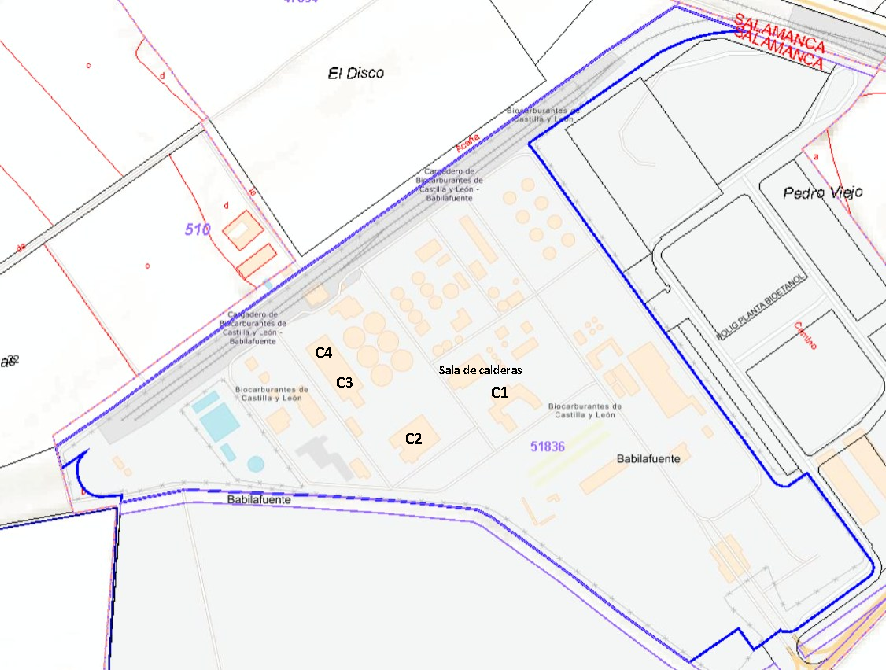
\includegraphics[width=0.85\textwidth]{Figuras/Plano_situacion.pdf}
	\caption{Emplazamiento de la parcela A3. Fuente: Proporcionada por el tutor.}
	\label{fig:plano-parcela}
\end{figure}

Respecto al tipo de instalación, cabe distinguir entre tramos aéreos y soterrados. Los tramos aéreos, que constituyen seis de los siete tramos de la red, discurren a una altura comprendida entre 5 y 6~m sobre el nivel del suelo, soportados mediante estructuras metálicas y con accesibilidad directa para labores de mantenimiento. El único tramo soterrado corresponde a la conexión P-C1, cuyo eje de tubería se sitúa a una profundidad de 1,09~m bajo la rasante del terreno. Este tramo soterrado requiere consideraciones especiales en cuanto al aislamiento térmico y la protección mecánica de la tubería, aspectos que serán desarrollados en las secciones correspondientes de la presente memoria.

\subsection{Puntos de consumo y requerimientos iniciales}
\label{subsec:puntos-consumo-requerimientos}

La instalación de vapor abastece a cuatro consumidores industriales (C1, C2, C3 y C4) con diferentes requerimientos de caudal y presión de operación. La caracterización precisa de estos puntos de consumo constituye el punto de partida para el dimensionamiento de la red de distribución, ya que determina tanto los caudales circulantes por cada tramo como las pérdidas de carga admisibles en el sistema.

Los datos de partida correspondientes a cada consumidor se presentan en la \tabref{tab:consumidores-requerimientos}, donde se indica el caudal demandado, la presión mínima requerida en el punto de consumo, la presión disponible tras considerar las pérdidas de carga en la red, y la distancia desde la caldera hasta cada punto de suministro.

\begin{table}[H]
	\centering
	\small
	\setlength{\tabcolsep}{3pt}
	\caption{Requerimientos de los puntos de consumo. Fuente: Elaboración grupal.}
	\label{tab:consumidores-requerimientos}
	\resizebox{\textwidth}{!}{
		\begin{tabular}{ccccc}
			\toprule
			\textbf{Consumidor} & \textbf{Caudal [kg/h]} & \textbf{Presión requerida [bar(g)]} & \textbf{Presión disponible [bar(g)]} & \textbf{Distancia [m]} \\
			\midrule
			C1                  & 679                    & 4                                   & 8,818                                & 100,93                 \\
			C2                  & 1359                   & 7                                   & 8,830                                & 143,74                 \\
			C3                  & 340                    & 7                                   & 8,710                                & 193,74                 \\
			C4                  & 2038                   & 7                                   & 8,690                                & 223,74                 \\
			\bottomrule
		\end{tabular}
	}
\end{table}

Del análisis de los datos presentados se desprende que el consumidor C4 representa el mayor demandante de vapor, con un caudal de 2038~kg/h que supone aproximadamente el 46\% del consumo total de la instalación. Por el contrario, el consumidor C3 presenta el menor requerimiento con tan solo 340~kg/h. Esta distribución heterogénea de caudales condiciona directamente el dimensionamiento de los diferentes tramos de la red.

\subsubsection{Cálculo del caudal total de diseño}

El caudal total de diseño de la instalación se determina a partir de la suma de los caudales individuales de cada consumidor, aplicando un factor de seguridad $K$ que contempla las pérdidas por fugas inherentes a cualquier red de distribución de vapor. El cálculo se realiza mediante la siguiente expresión:

\begin{equation}
	\begin{split}
		Q_{\text{total}} & = K \cdot \sum_{i=1}^{4} C_i                 \\
		                 & = 1{,}15 \cdot (679 + 1359 + 340 + 2038)     \\
		                 & = 1{,}15 \cdot 4416 = 5078{,}4 \ \text{kg/h}
	\end{split}
	\label{eq:caudal-total-diseno}
\end{equation}

El factor de seguridad adoptado, $K = 1{,}15$, corresponde a un incremento del 15\% sobre el caudal nominal calculado. Este margen adicional compensa las inevitables fugas de vapor que se producen en juntas, válvulas, purgadores y demás elementos de la instalación, asegurando que la capacidad de generación sea suficiente para satisfacer la demanda real del sistema en condiciones de operación continua.

El caudal de diseño calculado de 5078,4~kg/h se ajusta al caudal comercial de la caldera seleccionada. La \tabref{tab:resumen-caudales} presenta un resumen de los valores característicos del dimensionamiento.

\begin{table}[H]
	\centering
	\caption{Resumen del cálculo de caudales de diseño. Fuente: Elaboración grupal.}
	\label{tab:resumen-caudales}
	\begin{tabular}{lc}
		\toprule
		\textbf{Parámetro}                        & \textbf{Valor} \\
		\midrule
		Suma de caudales de consumidores          & 4416 [kg/h]    \\
		Factor de seguridad ($K$)                 & 1,15 [---]     \\
		Caudal de diseño calculado                & 5078,4 [kg/h]  \\
		Caudal comercial (caldera Vitomax 100-HS) & 5400 [kg/h]    \\
		\bottomrule
	\end{tabular}
\end{table}

\subsubsection{Condiciones del vapor de suministro}

El vapor generado por la caldera Viessmann VITOMAX 100-HS corresponde a vapor sobrecalentado, condición que se mantiene a lo largo de la red de distribución. Las propiedades termodinámicas del vapor a la salida de la caldera se recogen en la \tabref{tab:condiciones-vapor}.

\begin{table}[H]
	\centering
	\caption{Propiedades del vapor a la salida de la caldera. Fuente: Elaboración grupal.}
	\label{tab:condiciones-vapor}
	\begin{tabular}{lc}
		\toprule
		\textbf{Propiedad}          & \textbf{Valor} \\
		\midrule
		Tipo de vapor               & Sobrecalentado \\
		Temperatura [°C]            & 220            \\
		Presión de caldera [bar(g)] & 9,068          \\
		Entalpía específica [kJ/kg] & 2874           \\
		\bottomrule
	\end{tabular}
\end{table}

\subsubsection{Consideraciones especiales para el consumidor C1}

El análisis de los requerimientos de presión revela una diferencia significativa entre el consumidor C1 y el resto de puntos de consumo. Mientras que los consumidores C2, C3 y C4 operan a una presión de 7~bar(g), el consumidor C1 requiere una presión de trabajo de únicamente 4~bar(g).

Esta circunstancia, combinada con el hecho de que la presión disponible en el punto C1 es de 8,818~bar(g), implica la necesidad de instalar una válvula reductora de presión en el tramo de alimentación a dicho consumidor. La válvula reductora deberá ser capaz de reducir la presión desde aproximadamente 8,8~bar(g) hasta los 4~bar(g) requeridos, manteniendo una regulación estable ante variaciones de caudal.

Los requerimientos detallados en la presente sección constituyen la base para el dimensionamiento de la red de distribución de vapor que se desarrolla en las siguientes secciones de esta memoria técnica.

\section{Metodología}
\label{sec:metodologia}

La presente sección desarrolla la metodología empleada para el dimensionamiento de la instalación de vapor y condensados. Se abordan, en primer lugar, las bases de diseño que fundamentan los cálculos, incluyendo las propiedades del fluido de trabajo y los criterios de selección de equipos. Posteriormente, se detallan los procedimientos de cálculo aplicados a cada componente del sistema: línea de distribución de vapor, red de retorno de condensados, selección de caldera y dimensionamiento del aislamiento térmico.

\subsection{Bases de Diseño y Selección de Equipos Generales}
\label{subsec:bases-diseno}

En esta subsección se establecen los fundamentos técnicos que rigen el dimensionamiento de la instalación. Se definen las propiedades termodinámicas del vapor de trabajo, los criterios de velocidad máxima admisible en las tuberías, las pérdidas de carga permitidas y los factores de seguridad aplicados. Estos parámetros constituyen las restricciones de diseño que garantizan un funcionamiento seguro y eficiente del sistema.

\subsubsection{Propiedades del vapor utilizado}
\label{subsubsec:propiedades-vapor}

La instalación opera con vapor sobrecalentado generado por la caldera Viessmann VITOMAX 100-HS a una presión de 10~bar(a) y una temperatura de 220~°C. La selección de vapor sobrecalentado, en contraposición al vapor saturado, obedece a criterios técnicos que optimizan el transporte y la distribución del fluido térmico en instalaciones industriales de media y larga distancia.

El grado de sobrecalentamiento del vapor se define como la diferencia entre la temperatura real del vapor y su temperatura de saturación a la presión de trabajo. Para las condiciones de operación de la presente instalación:

\begin{equation}
	\Delta T_{\text{sob}} = T_{\text{vapor}} - T_{\text{sat}} = 220 - 180{,}2 = 39{,}8 \ \text{°C} \approx 40 \ \text{°C}
	\label{eq:grado-sobrecalentamiento}
\end{equation}

Este margen de sobrecalentamiento de aproximadamente 40~°C proporciona una reserva térmica que previene la condensación prematura del vapor durante su transporte a través de la red de distribución, especialmente en los tramos de mayor longitud donde las pérdidas de calor hacia el ambiente son más significativas.

Las propiedades termodinámicas del vapor sobrecalentado a las condiciones de operación (10~bar(a), 220~°C) se presentan en la \tabref{tab:propiedades-vapor-sobrecalentado}.

\begin{table}[H]
	\centering
	\caption{Propiedades termodinámicas del vapor sobrecalentado a 10~bar(a) y 220~°C. Fuente: Elaboración grupal.}
	\label{tab:propiedades-vapor-sobrecalentado}
	\begin{tabular}{lcc}
		\toprule
		\textbf{Propiedad}                   & \textbf{Símbolo} & \textbf{Valor}          \\
		\midrule
		Presión absoluta                     & $P$              & 10 [bar(a)]             \\
		Presión manométrica                  & $P_g$            & 9,068 [bar(g)]          \\
		Temperatura                          & $T$              & 220 [°C]                \\
		Temperatura de saturación            & $T_{\text{sat}}$ & 180,2 [°C]              \\
		Entalpía específica                  & $h_v$            & 2874 [kJ/kg]            \\
		Calor específico a presión constante & $c_p$            & 2,08 [kJ/(kg·K)]        \\
		Densidad                             & $\rho$           & 4,85 [kg/m³]            \\
		Volumen específico                   & $v$              & 0,206 [m³/kg]           \\
		Viscosidad dinámica                  & $\mu$            & 1,74 × 10$^{-5}$ [Pa·s] \\
		Viscosidad cinemática                & $\nu$            & 3,59 × 10$^{-6}$ [m²/s] \\
		\bottomrule
	\end{tabular}
\end{table}

La viscosidad cinemática, parámetro fundamental para el cálculo del número de Reynolds y, por tanto, para la determinación del régimen de flujo y las pérdidas de carga, se obtiene a partir de la viscosidad dinámica y la densidad del vapor mediante la relación:

\begin{equation}
	\nu = \frac{\mu}{\rho} = \frac{1{,}74 \times 10^{-5}}{4{,}85} = 3{,}59 \times 10^{-6} \ \text{m}^2\text{/s}
	\label{eq:viscosidad-cinematica}
\end{equation}

La selección de vapor sobrecalentado frente a vapor saturado se justifica por las siguientes ventajas técnicas:

\begin{enumerate}[label=\arabic*., leftmargin=2em]
	\item Mayor contenido energético: El vapor sobrecalentado presenta una entalpía específica superior (2874~kJ/kg) que permite transportar mayor cantidad de energía por unidad de masa.
	\item Reducción de condensados: El sobrecalentamiento minimiza la formación de condensados durante el transporte, evitando los problemas asociados al golpe de ariete y la corrosión en las tuberías.
	\item Mayor alcance de distribución: El margen térmico de 40~°C permite recorrer distancias más largas sin que el vapor alcance condiciones de saturación, característica especialmente relevante en esta instalación donde el tramo más largo supera los 220~m.
	\item Margen de seguridad operativo: El sobrecalentamiento proporciona un factor de seguridad frente a variaciones de carga o condiciones ambientales que podrían provocar condensación prematura en sistemas con vapor saturado.
\end{enumerate}

Estas propiedades termodinámicas constituyen los datos de entrada para los cálculos de dimensionamiento de tuberías, pérdidas de carga y selección de equipos que se desarrollan en las secciones subsiguientes de la presente memoria.


\subsubsection{Cálculo de la demanda total y márgenes de seguridad}
\label{subsubsec:demanda-total-margenes}

En la sección~\ref{subsec:puntos-consumo-requerimientos} se determinó el caudal de diseño de la instalación mediante la aplicación del factor de seguridad $K = 1{,}15$ sobre la suma de caudales de los consumidores. La presente sección profundiza en la justificación técnica de dicho factor, desarrolla el cálculo de la potencia térmica asociada y analiza el margen de reserva resultante de la capacidad de la caldera seleccionada.

\paragraph{Composición del margen de seguridad}

El factor de seguridad $K = 1{,}15$ adoptado en el dimensionamiento corresponde exclusivamente a la compensación de pérdidas por fugas en la red de distribución. La práctica industrial establece márgenes típicos comprendidos entre el 10\% y el 20\% para este concepto, habiéndose seleccionado un valor intermedio del 15\% acorde con instalaciones de vapor industrial de tamaño medio.

La decisión de no aplicar un factor de simultaneidad responde a un criterio de diseño conservador: se asume que todos los consumidores pueden operar de forma simultánea a su caudal nominal. En instalaciones con múltiples procesos independientes, la aplicación de factores de simultaneidad (típicamente entre 0,7 y 0,9) podría reducir el caudal de diseño, si bien requeriría un análisis detallado de los perfiles de consumo que excede el alcance del presente proyecto. Asimismo, dado que la instalación es existente y no se prevén ampliaciones futuras, no se ha considerado un factor de ampliación adicional. Finalmente, los transitorios de arranque, aunque pueden generar picos de demanda, no se han incluido en el cálculo del caudal de diseño, asumiendo que la caldera y la red de distribución están dimensionadas para operar en régimen permanente.

\paragraph{Cálculo de la potencia térmica}

La potencia térmica requerida por la instalación se determina mediante un balance entálpico entre las condiciones del vapor generado y el agua de alimentación a la caldera. La expresión general del balance energético es:

\begin{equation}
	P = \dot{m} \cdot (h_v - h_w)
	\label{eq:potencia-termica-balance}
\end{equation}

\noindent donde $P$ es la potencia térmica en kW, $\dot{m}$ es el caudal másico en kg/s, $h_v$ es la entalpía específica del vapor sobrecalentado y $h_w$ es la entalpía del agua de alimentación.

Para las condiciones de operación de la instalación, los valores de las entalpías son:

\begin{itemize}[leftmargin=2em]
	\item Entalpía del vapor sobrecalentado a 10~bar(a) y 220~°C: $h_v = 2874$~kJ/kg
	\item Entalpía del agua de alimentación a 15~°C: $h_w = 62{,}7$~kJ/kg
\end{itemize}

La diferencia de entalpías representa el calor aportado por la caldera para transformar el agua de alimentación en vapor sobrecalentado:

\begin{equation}
	\Delta h = h_v - h_w = 2874 - 62{,}7 = 2811{,}3 \ \text{kJ/kg}
	\label{eq:diferencia-entalpias}
\end{equation}

Para el caudal de diseño de la caldera (5400~kg/h), la potencia térmica resulta:

\begin{equation}
	P = \frac{5400}{3600} \times 2811{,}3 = 1{,}5 \times 2811{,}3 = 4217 \ \text{kW}
	\label{eq:potencia-caldera}
\end{equation}

\paragraph{Método alternativo: Factor f}

Un método simplificado para la estimación de la potencia térmica en instalaciones de vapor utiliza el denominado factor $f$, que relaciona directamente el caudal másico con la potencia térmica. Este factor depende de la presión de operación y se obtiene de gráficas normalizadas como la presentada en la \figref{fig:seleccion-factor-f}.

\begin{figure}[H]
	\centering
	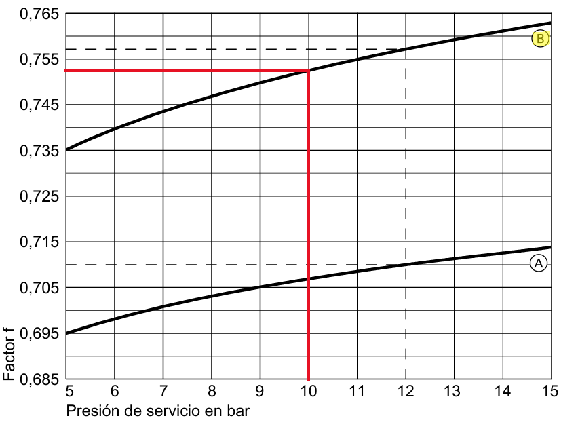
\includegraphics[width=0.75\textwidth]{Figuras/seleccion_factor_f.pdf}
	\caption{Gráfica para la determinación del factor $f$ en función de la presión de vapor. Fuente: Adaptada de \cite{VIESSMANN2013}.}
	\label{fig:seleccion-factor-f}
\end{figure}

Para una presión de 10~bar(a), el factor $f$ obtenido de la gráfica es aproximadamente $f = 0{,}753$~kW/(kg/h). La potencia térmica estimada mediante este método es:

\begin{equation}
	P_f = f \cdot Q = 0{,}753 \times 5400 = 4066 \ \text{kW}
	\label{eq:potencia-factor-f}
\end{equation}

La diferencia entre ambos métodos (4217~kW frente a 4066~kW) se debe a que el factor $f$ corresponde típicamente a vapor saturado, mientras que el balance entálpico considera las condiciones reales de vapor sobrecalentado. El método del balance entálpico proporciona un resultado más preciso y conservador para la instalación analizada.

\paragraph{Margen de reserva de la instalación}

La caldera Viessmann VITOMAX 100-HS seleccionada tiene una capacidad nominal de 5400~kg/h, valor que supera el caudal de diseño calculado de 5078,4~kg/h. La \tabref{tab:margen-reserva-instalacion} presenta la comparación entre la demanda de la instalación y la capacidad disponible de la caldera.

\begin{table}[H]
	\centering
	\caption{Comparación entre demanda y capacidad de la caldera. Fuente: Elaboración grupal.}
	\label{tab:margen-reserva-instalacion}
	\begin{tabular}{lccc}
		\toprule
		\textbf{Parámetro}              & \textbf{Demanda} & \textbf{Capacidad caldera} & \textbf{Margen} \\
		\midrule
		Caudal nominal (sin $K$)        & 4416~kg/h        & 5400~kg/h                  & +22,3\%         \\
		Caudal de diseño ($K = 1{,}15$) & 5078,4~kg/h      & 5400~kg/h                  & +6,3\%          \\
		Potencia térmica                & $\sim$3449~kW    & $\sim$4217~kW              & +22,3\%         \\
		\bottomrule
	\end{tabular}
\end{table}

El margen de reserva del 6,3\% sobre el caudal de diseño (equivalente al 22,3\% sobre el caudal nominal de los consumidores) garantiza la capacidad de la caldera para satisfacer la demanda en condiciones normales de operación, incluyendo las pérdidas por fugas consideradas en el factor $K$.

El margen de reserva calculado se considera adecuado para una instalación industrial de estas características, proporcionando flexibilidad operativa ante posibles variaciones de carga sin sobredimensionar excesivamente el equipo de generación. La capacidad excedente permite, además, absorber picos puntuales de demanda que pudieran producirse durante maniobras de puesta en marcha de los consumidores, aunque estos transitorios no han sido objeto de análisis específico en el presente proyecto.

\subsubsection{Selección de la caldera de vapor y condiciones de salida}
\label{subsubsec:seleccion-caldera-vitomax}

La selección de la caldera constituye una decisión de diseño fundamental que condiciona las prestaciones de toda la instalación de vapor. El equipo seleccionado debe satisfacer simultáneamente los requerimientos de caudal, presión y temperatura demandados por los consumidores, garantizando además un margen de reserva adecuado para absorber variaciones de carga y pérdidas inherentes al sistema.

\paragraph{Criterios de selección}

La determinación de la caldera apropiada para la instalación se ha realizado considerando los siguientes criterios técnicos:

\begin{enumerate}[label=\arabic*., leftmargin=2em]
	\item \textbf{Capacidad de producción:} El caudal nominal de la caldera debe ser igual o superior al caudal de diseño calculado (5078,4~kg/h), correspondiente al caudal de los consumidores mayorado por el factor de seguridad $K = 1{,}15$.
	\item \textbf{Presión de trabajo:} La presión de diseño de la caldera debe compensar las pérdidas de carga en la red de distribución, garantizando la presión mínima requerida en todos los puntos de consumo.
	\item \textbf{Tipo de vapor:} Capacidad de generar vapor sobrecalentado a 220~°C para minimizar la formación de condensados durante el transporte.
	\item \textbf{Tecnología y eficiencia:} Caldera pirotubular de alta eficiencia, diseñada para operación continua en aplicaciones industriales.
\end{enumerate}

\paragraph{Determinación de la presión de diseño}

La presión mínima requerida en la caldera se determina a partir de la presión máxima demandada por los consumidores, adicionando las pérdidas de carga previstas en la red de distribución. El proceso de cálculo se desarrolla de la siguiente manera:

\begin{itemize}[leftmargin=2em]
	\item Presión máxima requerida por los consumidores (C2, C3, C4): 7~bar(g)
	\item Pérdida de carga admisible en la red: 1~bar
	\item Presión mínima en caldera: $P_{\text{caldera}} = 7 + 1 = 8$~bar(g)
	\item Corrección por altitud (700~m, $P_{\text{atm}} = 0{,}932$~bar): $P_{\text{abs}} = 8 + 0{,}932 \approx 9$~bar(a)
	\item Ajuste según disponibilidad comercial: 10~bar(g)
\end{itemize}

La presión absoluta de trabajo resulta ser 10~bar(a), equivalente a 9,068~bar(g) una vez considerada la corrección por altitud del emplazamiento.

\begin{figure}[H]
	\centering
	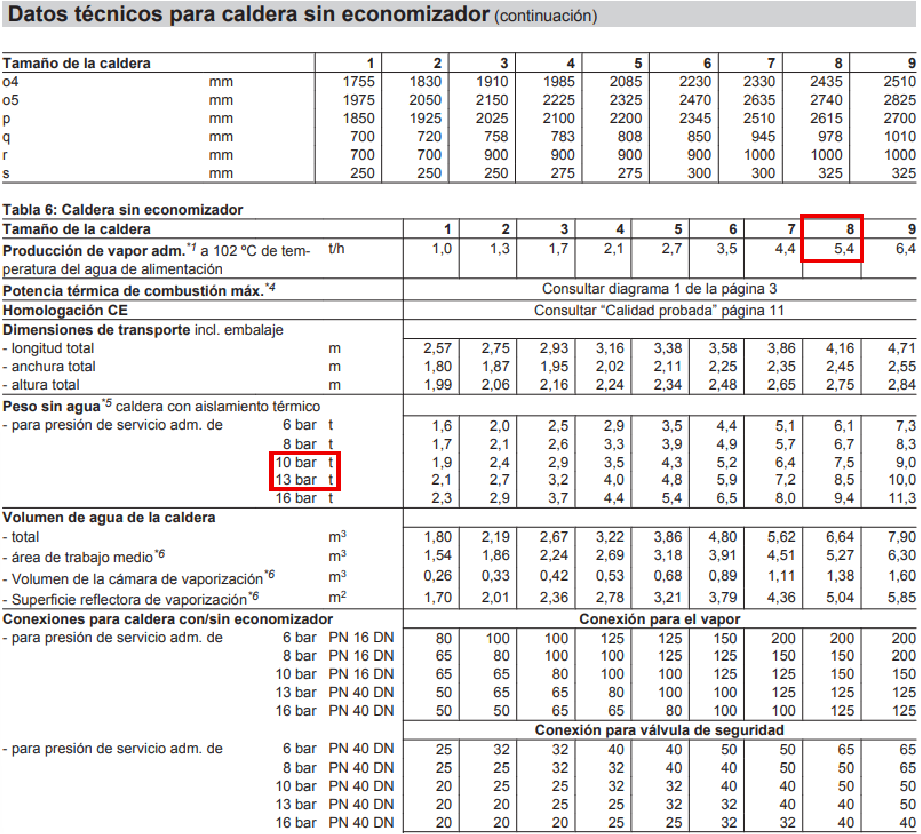
\includegraphics[width=0.75\textwidth]{Figuras/seleccion_presion.pdf}
	\caption{Determinación de la presión de diseño de la caldera. Fuente: Adaptada de \cite{VIESSMANN2013}.}
	\label{fig:seleccion-presion}
\end{figure}

\paragraph{Caldera seleccionada}

Tras el análisis del catálogo del fabricante Viessmann, se ha seleccionado la caldera VITOMAX 100-HS modelo M33A, cuyas especificaciones técnicas satisfacen los requerimientos de la instalación. La \tabref{tab:especificaciones-caldera-vitomax} recoge las características principales del equipo.

\begin{table}[H]
	\centering
	\caption{Especificaciones técnicas de la caldera Viessmann VITOMAX 100-HS M33A. Fuente: Elaboración grupal.}
	\label{tab:especificaciones-caldera-vitomax}
	\begin{tabular}{lc}
		\toprule
		\textbf{Parámetro}                        & \textbf{Valor} \\
		\midrule
		Fabricante                                & Viessmann      \\
		Serie                                     & VITOMAX 100-HS \\
		Modelo                                    & M33A           \\
		Tipo                                      & Pirotubular    \\
		Capacidad de producción de vapor [kg/h]   & 5400           \\
		Presión de diseño [bar(g)]                & 10             \\
		Presión absoluta de trabajo [bar(a)]      & 10             \\
		Temperatura de salida del vapor [°C]      & 220            \\
		Tipo de vapor                             & Sobrecalentado \\
		Temperatura del agua de alimentación [°C] & 15             \\
		\bottomrule
	\end{tabular}
\end{table}

La elección de la caldera VITOMAX 100-HS modelo M33A se justifica por las siguientes razones técnicas:

\begin{enumerate}[label=\arabic*., leftmargin=2em]
	\item Capacidad adecuada: El caudal comercial de 5400~kg/h es el inmediatamente superior al caudal de diseño calculado de 5078,4~kg/h, proporcionando un margen de reserva del 6,3\% adicional.
	\item Presión suficiente: La presión de diseño de 10~bar(g) garantiza que, tras las pérdidas de carga en la red (máximo 0,38~bar hasta el consumidor más desfavorable C4), todos los puntos de consumo recibirán vapor a la presión requerida.
	\item Tecnología apropiada: La caldera pirotubular de alta eficiencia está diseñada para operación continua en aplicaciones industriales, con alta fiabilidad y bajo mantenimiento.
	\item Disponibilidad comercial: El modelo existe en el catálogo actual del fabricante Viessmann, garantizando el suministro de repuestos y servicio técnico.
\end{enumerate}

La \tabref{tab:comparacion-demanda-caldera} presenta la comparación detallada entre la demanda de la instalación y la capacidad de la caldera seleccionada.

\begin{table}[H]
	\centering
	\caption{Comparación entre la demanda de la instalación y la capacidad de la caldera. Fuente: Elaboración grupal.}
	\label{tab:comparacion-demanda-caldera}
	\begin{tabular}{lc}
		\toprule
		\textbf{Concepto}                   & \textbf{Valor} \\
		\midrule
		Caudal nominal total (C1+C2+C3+C4)  & 4416 [kg/h]    \\
		Factor de seguridad por fugas ($K$) & 1,15           \\
		Caudal de diseño                    & 5078,4 [kg/h]  \\
		Caudal comercial de la caldera      & 5400 [kg/h]    \\
		Margen de reserva disponible        & 321,6 [kg/h]   \\
		Margen de reserva porcentual        & 6,3 [\%]       \\
		\bottomrule
	\end{tabular}
\end{table}

\paragraph{Propiedades termodinámicas del vapor a la salida}

El vapor generado por la caldera VITOMAX 100-HS abandona el equipo en condiciones de sobrecalentamiento. Las propiedades termodinámicas del vapor a la salida de la caldera se recogen en la \tabref{tab:condiciones-salida-caldera}.

\begin{table}[H]
	\centering
	\caption{Condiciones del vapor a la salida de la caldera. Fuente: Elaboración grupal.}
	\label{tab:condiciones-salida-caldera}
	\begin{tabular}{lc}
		\toprule
		\textbf{Propiedad}                   & \textbf{Valor} \\
		\midrule
		Presión absoluta [bar(a)]            & 10             \\
		Presión manométrica [bar(g)]         & 9,068          \\
		Temperatura del vapor [°C]           & 220            \\
		Estado del vapor                     & Sobrecalentado \\
		Temperatura de saturación [°C]       & 180            \\
		Entalpía específica ($h_v$) [kJ/kg]  & 2874           \\
		Densidad ($\rho$) [kg/m³]            & 4,85           \\
		Calor específico ($c_p$) [kJ/(kg·K)] & 2,08           \\
		\bottomrule
	\end{tabular}
\end{table}

El grado de sobrecalentamiento de aproximadamente 40~°C (diferencia entre la temperatura real del vapor, 220~°C, y la temperatura de saturación a 10~bar(a), aproximadamente 180~°C) proporciona un margen térmico adecuado para prevenir la condensación prematura del vapor durante su transporte a través de la red de distribución.

\paragraph{Cálculo de la potencia térmica}

La potencia térmica de la caldera se determina mediante el balance entálpico entre las condiciones del vapor generado y el agua de alimentación:

\begin{equation}
	P = \dot{m} \cdot (h_v - h_w)
	\label{eq:potencia-termica-caldera}
\end{equation}

\noindent donde $\dot{m}$ es el caudal másico (kg/s), $h_v$ es la entalpía del vapor sobrecalentado (kJ/kg) y $h_w$ es la entalpía del agua de alimentación (kJ/kg).

Sustituyendo los valores correspondientes a las condiciones de operación:

\begin{equation}
	P = \frac{5400}{3600} \times (2874 - 62{,}7) = 1{,}5 \times 2811{,}3 = 4217 \ \text{kW}
	\label{eq:potencia-caldera-calculada}
\end{equation}

La potencia térmica de 4217~kW corresponde a la capacidad nominal de la caldera operando a su caudal máximo de 5400~kg/h. Para el caudal nominal de los consumidores (4416~kg/h, sin considerar el factor $K$), la potencia requerida sería:

\begin{equation}
	P_{\text{nominal}} = \frac{4416}{3600} \times 2811{,}3 = 1{,}227 \times 2811{,}3 = 3449 \ \text{kW}
	\label{eq:potencia-nominal-consumidores}
\end{equation}

La \tabref{tab:resumen-potencias-caldera} presenta el resumen de las potencias térmicas calculadas para los distintos escenarios de operación.

\begin{table}[H]
	\centering
	\caption{Resumen de potencias térmicas según escenario de operación. Fuente: Elaboración grupal.}
	\label{tab:resumen-potencias-caldera}
	\begin{tabular}{lccc}
		\toprule
		\textbf{Escenario}            & \textbf{Caudal [kg/h]} & \textbf{Caudal [kg/s]} & \textbf{Potencia [kW]} \\
		\midrule
		Caudal nominal consumidores   & 4416                   & 1,227                  & 3449                   \\
		Caudal de diseño ($K=1{,}15$) & 5078,4                 & 1,411                  & 3966                   \\
		Capacidad nominal caldera     & 5400                   & 1,500                  & 4217                   \\
		\bottomrule
	\end{tabular}
\end{table}

\paragraph{Representación gráfica}

La \figref{fig:ficha-caldera-vitomax} muestra un extracto de la ficha técnica del fabricante correspondiente a la caldera seleccionada.

\begin{figure}[H]
	\centering
	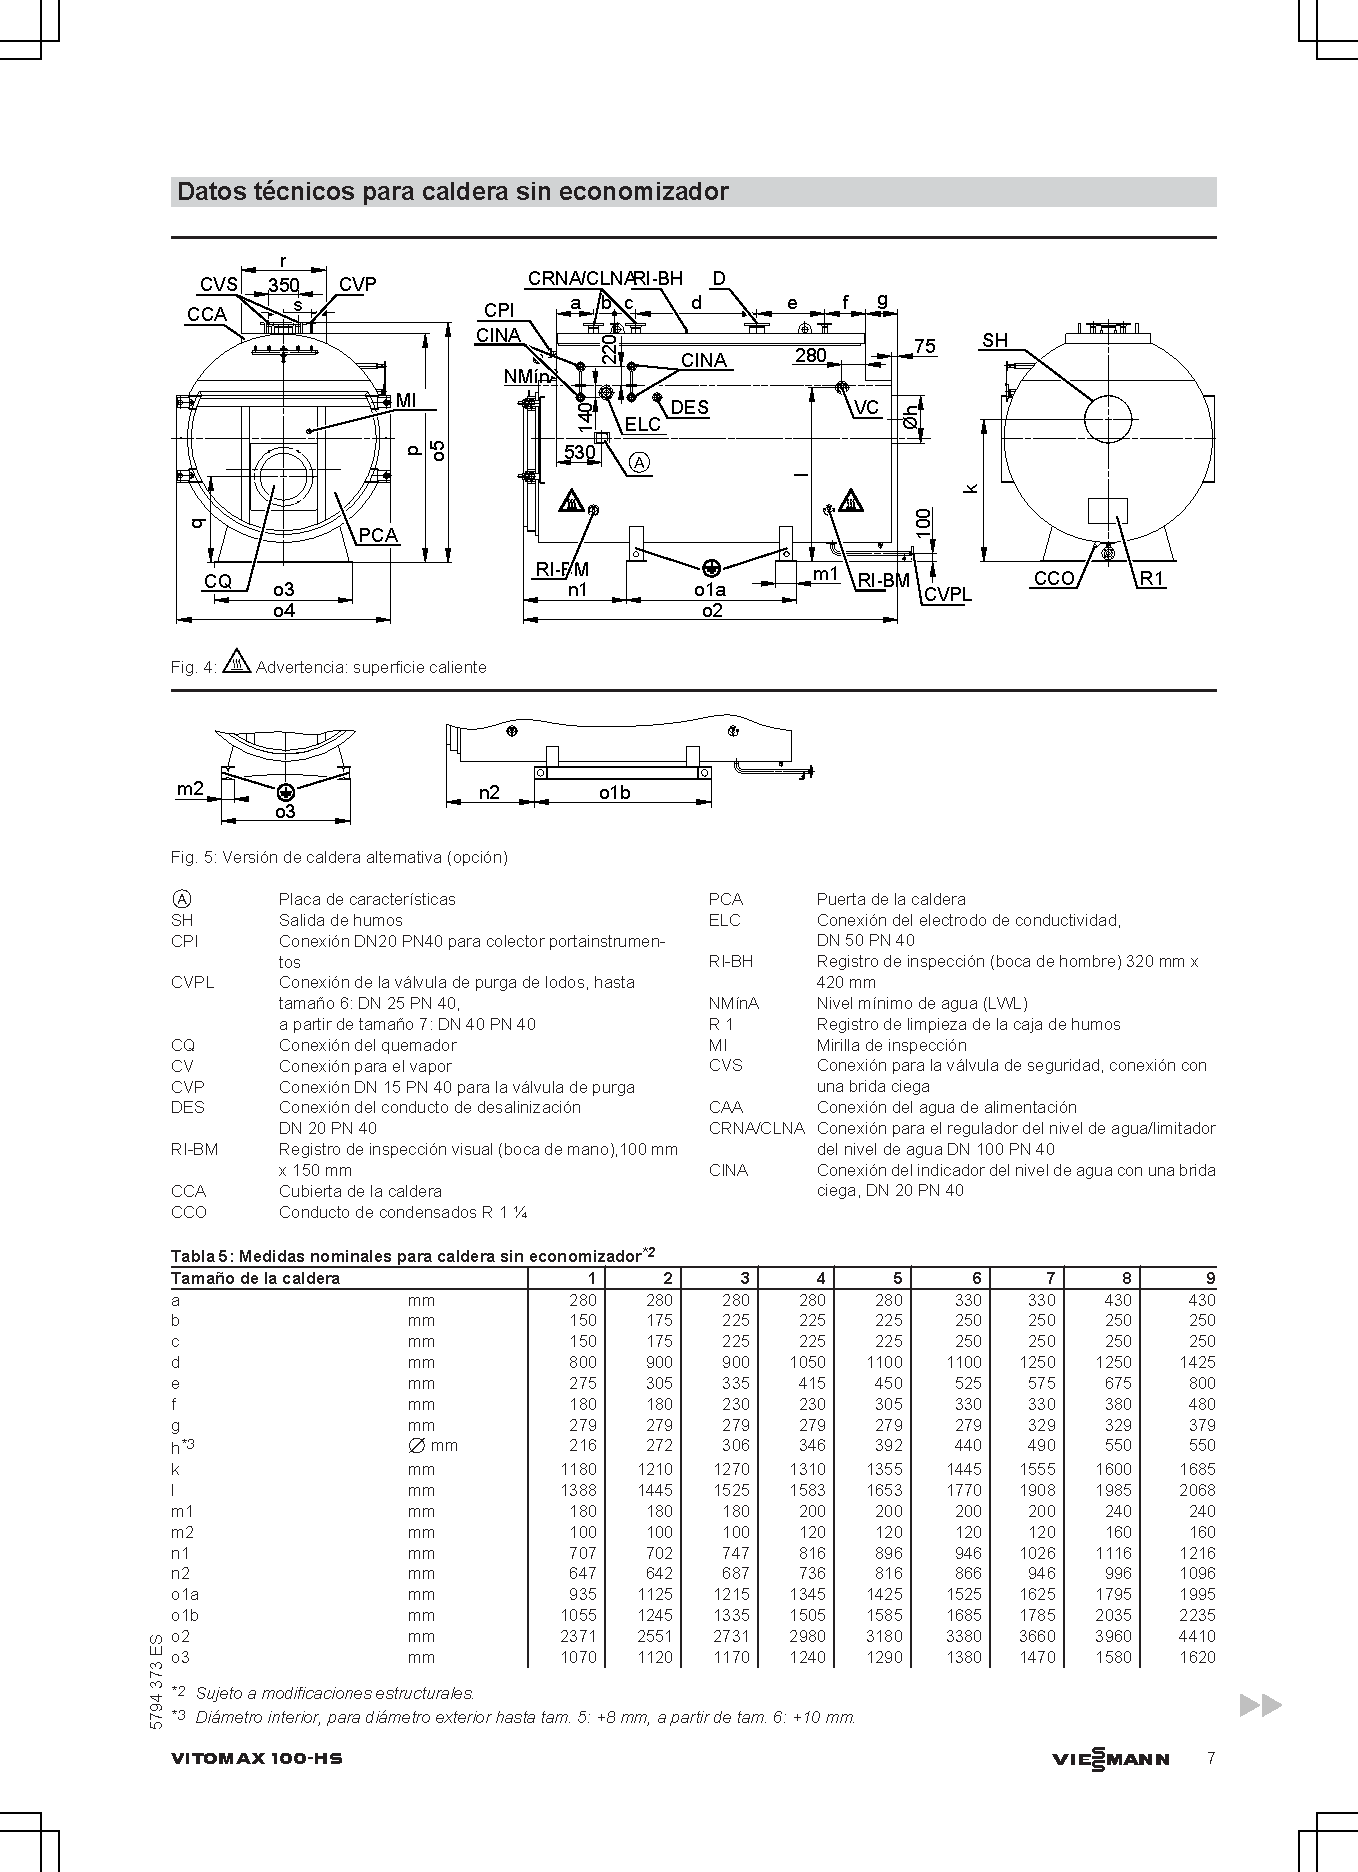
\includegraphics[trim={3cm 21cm 15.3cm 4.2cm}, clip, keepaspectratio, width=0.45\textwidth]{Figuras/Vitomax_100HS_33-A.pdf}
	\caption{Esquema de la caldera Viessmann VITOMAX 100-HS M33A (sin economizador). Fuente: Adaptada de \cite{VIESSMANN2013}.}
	\label{fig:ficha-caldera-vitomax}
\end{figure}

Las condiciones de salida de la caldera (10~bar(a), 220~°C, vapor sobrecalentado) constituyen el punto de partida para el dimensionamiento de la red de distribución de vapor que se desarrolla en las secciones subsiguientes de la presente memoria técnica.

\newpage

\subsection{Dimensionado Hidráulico de la Red de Vapor}
\label{subsec:dimensionado-red-vapor}

El dimensionado hidráulico de la red de distribución de vapor constituye una etapa fundamental del proyecto, cuyo objetivo es determinar los diámetros de tubería apropiados para cada tramo de la instalación. El proceso de dimensionado debe garantizar que el sistema opere dentro de límites técnicos y económicos aceptables, asegurando el suministro de vapor a todos los puntos de consumo con las condiciones de presión y caudal requeridas.

El dimensionado se aborda mediante un procedimiento sistemático que parte de los criterios de diseño establecidos en la normativa de referencia, aplica las ecuaciones fundamentales de la mecánica de fluidos y verifica el cumplimiento de las restricciones impuestas. Los criterios adoptados buscan un equilibrio entre el coste de la instalación (diámetros pequeños) y las pérdidas de carga asociadas (diámetros grandes), optimizando el funcionamiento global del sistema.

\subsubsection{Criterios de dimensionado}
\label{subsubsec:criterios-dimensionado}

El dimensionado de las tuberías de vapor se fundamenta en tres criterios principales: la velocidad máxima admisible del fluido, la caída de presión total permitida en la red y la rugosidad del material de las tuberías. Estos criterios, establecidos a partir de la normativa y guías técnicas de referencia (RITE \cite{RITE2007}, Manual EREN \cite{EREN2015}, Guía Spirax Sarco \cite{SpiraxSarco2020}), definen las restricciones que debe cumplir el diseño para garantizar un funcionamiento seguro y eficiente de la instalación.

\paragraph{Distribución de caudales en la red}

La red de distribución de vapor presenta una topología ramificada que parte de la caldera y se bifurca progresivamente en los nodos P, S y T para alimentar a los cuatro consumidores. La determinación de los caudales circulantes por cada tramo requiere un análisis sistemático de la red, partiendo del caudal total generado y aplicando un balance de masas en cada punto de bifurcación.

El caudal total de diseño de la instalación, incluyendo el factor de seguridad del 15\% por fugas, es de 5400~kg/h. Este caudal se distribuye progresivamente en los nodos de bifurcación según la demanda de cada consumidor. 

Los caudales de diseño de cada tramo de la red se determinan sustrayendo del caudal total disponible en caldera (5400 kg/h) el consumo de los puntos de suministro mayorados por el factor de seguridad individual (K=1,15). El desarrollo matemático para los siete tramos es el siguiente:

\begin{align}
	\dot{m}_{\mathrm{TR1}} & = 5400\;\text{kg/h} \quad \text{(caudal total de diseño a la salida de caldera)} \\
	\dot{m}_{\mathrm{TR2}} & = 5400 - 1{,}15 \cdot (1359 + 340 + 2038) = 1102{,}45\;\text{kg/h}               \\
	\dot{m}_{\mathrm{TR3}} & = 5400 - 1{,}15 \cdot 679 = 4619{,}15\;\text{kg/h}                               \\
	\dot{m}_{\mathrm{TR4}} & = 5400 - 1{,}15 \cdot (679 + 340 + 2038) = 1884{,}45\;\text{kg/h}                \\
	\dot{m}_{\mathrm{TR5}} & = 5400 - 1{,}15 \cdot (679 + 1359) = 3056{,}3\;\text{kg/h}                       \\
	\dot{m}_{\mathrm{TR6}} & = 5400 - 1{,}15 \cdot (679 + 1359 + 2038) = 712{,}6\;\text{kg/h}                 \\
	\dot{m}_{\mathrm{TR7}} & = 5400 - 1{,}15 \cdot (679 + 1359 + 340) = 2665{,}3\;\text{kg/h}
\end{align}


\paragraph{Criterio de velocidad}

La velocidad del vapor en el interior de las tuberías constituye el parámetro de control principal en el dimensionado de redes de distribución. Una velocidad excesivamente alta provoca efectos indeseables que comprometen la integridad y el funcionamiento del sistema:

\begin{itemize}[leftmargin=2em]
	\item \textbf{Erosión en codos y accesorios:} Las partículas de condensado arrastradas por el vapor a alta velocidad impactan contra las paredes internas de los accesorios, provocando un desgaste progresivo del material.
	\item \textbf{Incremento del nivel de ruido:} Velocidades elevadas generan turbulencias y vibraciones que se traducen en niveles de ruido inaceptables en entornos industriales.
	\item \textbf{Mayores pérdidas de carga:} La pérdida de presión por fricción es proporcional al cuadrado de la velocidad, por lo que velocidades altas incrementan significativamente las pérdidas energéticas.
	\item \textbf{Riesgo de vibraciones y fatiga mecánica:} Las fluctuaciones de presión asociadas a flujos turbulentos a alta velocidad pueden inducir vibraciones en las tuberías y sus soportes, acelerando la fatiga del material.
\end{itemize}

Para la presente instalación se ha adoptado una velocidad de diseño de aproximadamente 20~m/s, valor que permite compatibilizar un diámetro de tubería con pérdidas de carga moderadas y un funcionamiento hidráulico adecuado. Este valor se encuentra dentro del rango recomendado por las guías técnicas de referencia para líneas de vapor industrial.

Para la presente instalación, que opera a una presión de 10~bar(a) con tramos de longitud considerable (hasta 223,74~m hasta el consumidor más alejado C4), la velocidad de diseño de 20~m/s representa un valor conservador que prioriza la minimización de pérdidas de carga. Como criterio de seguridad adicional, se establece una velocidad máxima  de 30~m/s que no debe superarse en ningún tramo de la instalación.

\paragraph{Criterio de caída de presión}

El segundo criterio de dimensionado establece la pérdida de carga máxima admisible en la red de distribución. Este límite garantiza que todos los puntos de consumo reciban vapor a la presión mínima requerida, considerando la presión disponible a la salida de la caldera.

Para la presente instalación se ha adoptado un criterio de pérdida de carga máxima de 1~bar por recorrido completo desde la caldera hasta el consumidor más desfavorable. Este criterio permite establecer la presión mínima requerida en la caldera:

\begin{equation}
	P_{\text{caldera}} = P_{\text{máx,consumidor}} + \Delta P_{\text{red}} = 7 + 1 = 8 \ \text{bar(g)}
	\label{eq:presion-minima-caldera}
\end{equation}

La caldera seleccionada opera a una presión efectiva de 9,068~bar(g), lo que proporciona un margen disponible para pérdidas de carga de:

\begin{equation}
	\Delta P_{\text{disponible}} = P_{\text{caldera}} - P_{\text{máx,consumidor}} = 9{,}068 - 7 = 2{,}068 \ \text{bar}
	\label{eq:margen-presion-disponible}
\end{equation}

Este margen, superior al criterio de diseño de 1~bar, proporciona una reserva de presión que permite absorber variaciones de carga y posibles obstrucciones parciales en la red sin comprometer el suministro a los consumidores.

Las pérdidas de carga en la red se calculan mediante la ecuación de \textbf{Darcy-Weisbach}, expresión fundamental de la mecánica de fluidos para el cálculo de pérdidas por fricción en conductos:

\begin{equation}
	\Delta P = f \cdot \frac{L}{D} \cdot \frac{\rho \cdot v^2}{2}
	\label{eq:darcy-weisbach}
\end{equation}


El factor de fricción $f$ depende del número de Reynolds y de la rugosidad relativa de la tubería ($\varepsilon/D$), obteniéndose mediante el diagrama de Moody o mediante correlaciones empíricas como la ecuación de Colebrook-White para régimen turbulento.

\paragraph{Rugosidad y material de tuberías}

El tercer criterio de dimensionado hace referencia a las características del material de las tuberías, que determinan la rugosidad superficial y, por tanto, las pérdidas de carga por fricción.

Para la presente instalación se ha seleccionado tubería de acero al carbono sin soldadura, material de uso generalizado en redes de vapor industrial por su resistencia mecánica, durabilidad y coste competitivo. Las tuberías se dimensionan de acuerdo con las siguientes normas técnicas:

\begin{itemize}[leftmargin=2em]
	\item DIN 2448 \cite{DIN2448}: Norma europea para tuberías de acero sin soldadura, de aplicación preferente para los diámetros nominales empleados en la instalación (DN~50 a DN~150).
	\item Sistema Schedule (API) \cite{API605}: Sistema americano que define el espesor de pared en función de la presión de trabajo. Se adopta Schedule~40 como estándar de diseño (para presiones hasta 10~bar(g)). Sin embargo, en función de los requirimientos de resistencia mecánica y las condiciones de operación, se podrían considerar espesores mayores como Schedule~80 o incluso Schedule~160 para tramos críticos o con mayores riesgos de erosión.
\end{itemize}

Para los cálculos de las instalación se usará una rugosidad absoluta ($\varepsilon$) de 0,02~mm. Este valor es representativo de tuberías de acero comercial nuevo.

Los diámetros normalizados según la norma DIN~2448 \cite{DIN2448} serán utilizados para la selección de tuberías comerciales en cada tramo de la instalación.

\paragraph{Ecuaciones fundamentales de dimensionado}

El dimensionado de cada tramo de la red se realiza mediante la aplicación de las ecuaciones fundamentales de la mecánica de fluidos, partiendo del caudal demandado y la velocidad objetivo para determinar el diámetro teórico, que posteriormente se ajusta al diámetro comercial normalizado.

La ecuación de continuidad permite calcular el diámetro teórico de la tubería a partir del caudal volumétrico y la velocidad de diseño:

\begin{equation}
	D = \sqrt{\frac{4 \cdot \dot{V}}{\pi \cdot C}}
	\label{eq:continuidad-diametro}
\end{equation}

\noindent donde:
\begin{itemize}[leftmargin=2em, label={}]
	\item $D$ = diámetro interior teórico [m]
	\item $\dot{V}$ = caudal volumétrico [m³/s]
	\item $C$ = velocidad objetivo [m/s]
\end{itemize}

El caudal volumétrico se obtiene a partir del caudal másico y la densidad del vapor:

\begin{equation}
	\dot{V} = \frac{\dot{m}}{\rho}
	\label{eq:caudal-volumetrico}
\end{equation}

Para el cálculo de las pérdidas de carga, la longitud de cálculo debe incluir tanto la longitud real de la tubería como las longitudes equivalentes de los accesorios presentes en el tramo:

\begin{equation}
	L_{\text{cálculo}} = L_{\text{real}} + L_{\text{eq}}
	\label{eq:longitud-calculo}
\end{equation}

Las longitudes equivalentes de los accesorios se expresan habitualmente como múltiplos del diámetro interior de la tubería ($L_e/D$). Los coeficientes $L_e/D$ dependen fundamentalmente de la geometría del accesorio y del régimen de flujo, y se han adoptado de acuerdo con el Manual Técnico de Diseño y Cálculo de Redes de Vapor \cite{EREN2015}.


La \figref{fig:tabla-perdidas-accesorios} muestra la tabla de referencia del Manual EREN con los valores de $L_e/D$ para diferentes accesorios y condiciones de instalación.

\begin{figure}[H]
	\centering
	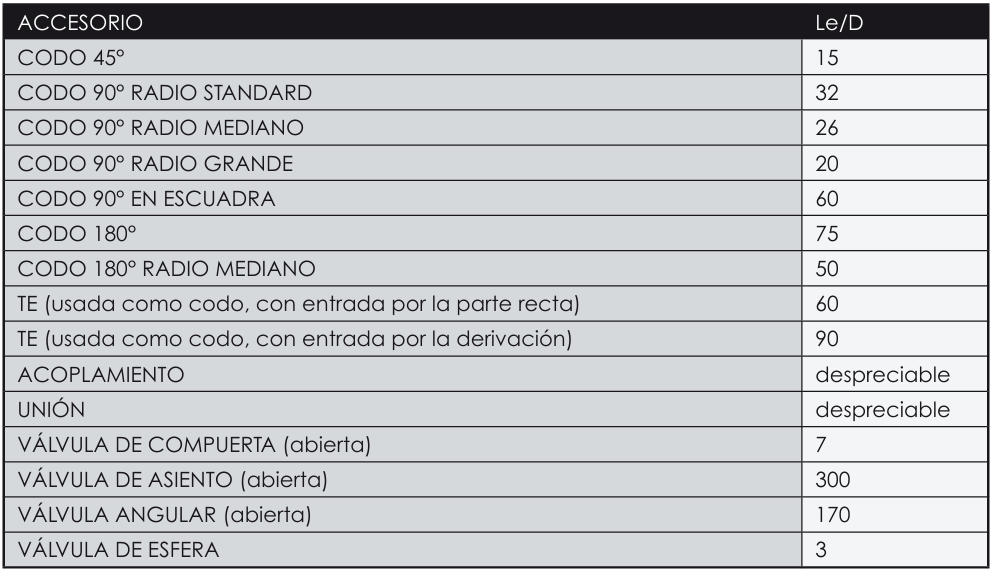
\includegraphics[width=0.85\textwidth]{Figuras/perdidas_carga_accesorios.png}
	\caption{Pérdidas de carga en accesorios expresadas como $L_e/D$. Fuente: Adaptado de \cite{EREN2015}.}
	\label{fig:tabla-perdidas-accesorios}
\end{figure}

\paragraph{Selección del tipo de codo}

Para la presente instalación se han seleccionado codos de radio mediano ($R \approx 1{,}5 \cdot D$) con un coeficiente $L_e/D = 26$. Esta elección se justifica por las siguientes ventajas técnicas frente al codo de radio estándar:

\begin{enumerate}[label=\arabic*., leftmargin=2em]
	\item \textbf{Reducción de pérdidas de carga:} El codo de radio mediano presenta un coeficiente $L_e/D = 26$, frente a los 32 del codo de radio estándar. Esta diferencia supone una reducción de aproximadamente el 18\% en las pérdidas locales generadas por cada codo.
	\item \textbf{Mejora del perfil de velocidades:} El mayor radio de curvatura reduce las turbulencias en el interior del codo, mejorando el perfil de velocidades aguas abajo y minimizando los efectos de erosión sobre las paredes internas.
	\item \textbf{Recomendación técnica:} Las guías de diseño de redes de vapor (EREN \cite{EREN2015}, Spirax Sarco \cite{SpiraxSarco2020}) recomiendan el uso de codos de radio mediano o grande en líneas principales, reservando los codos de radio estándar para derivaciones secundarias o restricciones de espacio.
\end{enumerate}

El incremento de coste asociado al codo de radio mediano queda justificado por la reducción de pérdidas de carga y la mejora de las condiciones de operación de la instalación.

\paragraph{Aplicación y resumen de longitudes de cálculo}

La \tabref{tab:resumen-longitudes-calculo} presenta el inventario de accesorios identificados en cada tramo y resume el cálculo de las longitudes equivalentes resultantes. En los tramos que no presentan accesorios significativos (Caldera-P, S-C2 y T-C3), se ha aplicado un criterio simplificado mayorando la longitud real en un 20\% para contabilizar uniones y pequeños elementos. Para el resto de tramos, la longitud equivalente se ha determinado mediante la suma de los coeficientes $L_e/D$ y el diámetro de tanteo correspondiente.

\begin{table}[H]
	\centering
	\small
	\setlength{\tabcolsep}{3pt}
	\caption{Inventario de accesorios y resumen de longitudes de cálculo para la red de vapor. Fuente: Elaboración grupal.}
	\label{tab:resumen-longitudes-calculo}
	\resizebox{\textwidth}{!}{
		\begin{tabular}{lcccccccl}
			\toprule
			\textbf{Tramo} & \textbf{$L_{\text{real}}$ [m]} & \textbf{Codos 90°} & \textbf{T (recta)} & \textbf{T (deriv.)} & \textbf{$D_{\text{tant}}$ [mm]} & \textbf{$L_{\text{eq}}$ [m]} & \textbf{$L_{\text{calc}}$ [m]} & \textbf{Método} \\
			\midrule
			Caldera-P      & 12,74                          & 0                  & 0                  & 0                   & ---                             & 2,55                         & 15,29                          & Criterio 20\%   \\
			P-C1           & 88,19                          & 2                  & 1                  & 0                   & 60                              & 9,24                         & 97,43                          & $L_e/D$         \\
			P-S            & 106                            & 1                  & 0                  & 2                   & 120                             & 25,44                        & 131,44                         & $L_e/D$         \\
			S-C2        & 25                             & 0                  & 0                  & 0                   & ---                             & 5,00                         & 30,00                          & Criterio 20\%   \\
			S-T            & 60                             & 0                  & 1                  & 1                   & 120                             & 7,50                         & 78,00                          & $L_e/D$         \\
			T-C3        & 15                             & 0                  & 0                  & 0                   & ---                             & 3,00                         & 18,00                          & Criterio 20\%   \\
			T-C4        & 45                             & 2                  & 1                  & 0                   & 100                             & 12,40                        & 57,40                          & $L_e/D$         \\
			\midrule
			\textbf{Total} & \textbf{351,93}                & \textbf{5}         & \textbf{3}         & \textbf{3}          & ---                             & \textbf{65,13}               & \textbf{427,56}                & ---             \\
			\bottomrule
		\end{tabular}
	}
\end{table}

Las longitudes equivalentes calculadas representan un incremento medio del 18,5\% sobre las longitudes reales de la instalación. Este porcentaje se encuentra dentro del rango habitual para redes de vapor industrial con un número moderado de accesorios. Las longitudes de cálculo obtenidas serán empleadas en los cálculos de pérdida de carga que se desarrollan en las secciones posteriores de la presente memoria.

\subsubsection{Tramo 1: Caldera-P}
\label{subsubsec:tramo1-caldera-p}

El Tramo~1 constituye la línea principal de salida de la caldera, conectando el equipo generador con el primer nodo de bifurcación (punto~P) de la red de distribución. Este tramo transporta el 100\% del caudal de vapor generado, por lo que su correcto dimensionamiento resulta crítico para el funcionamiento global de la instalación.

\paragraph{Datos de partida}

El tramo Caldera-P presenta las características geométricas y de operación recogidas en la \tabref{tab:datos-partida-tramo1}.

\begin{table}[H]
	\centering
	\caption{Datos de partida para el Tramo 1 (Caldera-P). Fuente: Elaboración grupal.}
	\label{tab:datos-partida-tramo1}
	\begin{tabular}{lc}
		\toprule
		\textbf{Parámetro}          & \textbf{Valor}  \\
		\midrule
		Identificación              & TR1 (Caldera-P) \\
		Longitud real [m]           & 12,74           \\
		Longitud equivalente [m]    & 2,548           \\
		Longitud de cálculo [m]     & 15,288          \\
		Caudal másico [kg/h]        & 5400            \\
		Caudal másico [kg/s]        & 1,5             \\
		Presión de entrada [bar(g)] & 9,068           \\
		Temperatura [°C]            & 220             \\
		Tipo de tramo               & Aéreo           \\
		\bottomrule
	\end{tabular}
\end{table}

Este tramo no presenta accesorios significativos (0~codos, 0~derivaciones en~T), por lo que la longitud equivalente se ha calculado aplicando el criterio del 20\% sobre la longitud real:

\begin{equation}
	L_{\text{eq}} = 0{,}20 \times L_{\text{real}} = 0{,}20 \times 12{,}74 = 2{,}548 \ \text{m}
	\label{eq:Leq-tramo1}
\end{equation}

El caudal m\'asico de dise\~no para el tramo se obtiene directamente como el caudal total generado en caldera:

\begin{equation}
	\dot{m}_{\text{TR1}} = \dot{m}_{\text{total}} = 5400~\text{kg/h} = 1{,}5~\text{kg/s}
	\label{eq:caudal-tramo1}
\end{equation}

Las propiedades del vapor sobrecalentado a las condiciones de operación (10~bar(a), 220~°C) se presentan en la \tabref{tab:propiedades-vapor-tramo1}.

\begin{table}[H]
	\centering
	\caption{Propiedades del vapor en el Tramo 1. Fuente: Elaboración grupal.}
	\label{tab:propiedades-vapor-tramo1}
	\begin{tabular}{lcc}
		\toprule
		\textbf{Propiedad}    & \textbf{Símbolo} & \textbf{Valor}                 \\
		\midrule
		Densidad              & $\rho$           & 4,85 [kg/m³]                   \\
		Volumen específico    & $v$              & 0,206 [m³/kg]                  \\
		Viscosidad dinámica   & $\mu$            & 1,74 $\times$ 10$^{-5}$ [Pa·s] \\
		Viscosidad cinemática & $\nu$            & 3,59 $\times$ 10$^{-6}$ [m²/s] \\
		\bottomrule
	\end{tabular}
\end{table}

El caudal m\'asico de dise\~no del tramo se obtiene como:

\begin{equation}
	\dot{m}_{\text{TR2}} = \dot{m}_{\text{C1}} = 679~\text{kg/h}
	\label{eq:caudal-tramo2}
\end{equation}

\paragraph{Cálculo del diámetro}

El dimensionado del tramo parte del cálculo del caudal volumétrico a partir del caudal másico y la densidad del vapor:

\begin{equation}
	\dot{V} = \frac{\dot{m}}{\rho} = \frac{1{,}5}{4{,}85} = 0{,}309 \ \text{m}^3\text{/s}
	\label{eq:caudal-volumetrico-tramo1}
\end{equation}

Para la velocidad objetivo de 20~m/s, el área de paso requerida resulta:

\begin{equation}
	A = \frac{\dot{V}}{C} = \frac{0{,}309}{20} = 0{,}01545 \ \text{m}^2
	\label{eq:area-paso-tramo1}
\end{equation}

El diámetro teórico se obtiene a partir de la ecuación de continuidad:

\begin{equation}
	D_{\text{teórico}} = \sqrt{\frac{4 \cdot A}{\pi}} = \sqrt{\frac{4 \times 0{,}01545}{\pi}} = 0{,}1402 \ \text{m} = 140{,}2 \ \text{mm}
	\label{eq:diametro-teorico-tramo1}
\end{equation}

Consultando los diámetros normalizados según DIN~2448 \cite{DIN2448}, se selecciona el diámetro comercial inmediatamente superior: \textbf{DN~150 Schedule~80}.

La \tabref{tab:seleccion-tuberia-tramo1} recoge las características de la tubería seleccionada.

\begin{table}[H]
	\centering
	\caption{Características de la tubería seleccionada para el Tramo 1. Fuente: Elaboración grupal.}
	\label{tab:seleccion-tuberia-tramo1}
	\begin{tabular}{lc}
		\toprule
		\textbf{Parámetro}     & \textbf{Valor}    \\
		\midrule
		Diámetro nominal       & DN 150            \\
		Norma de referencia    & Schedule 80 [API] \\
		Diámetro exterior [mm] & 168,3             \\
		Espesor de pared [mm]  & 10,95             \\
		Diámetro interior [mm] & 146,4             \\
		\bottomrule
	\end{tabular}
\end{table}

\paragraph{Justificación del Schedule 80}

Para el tramo de salida de caldera se ha seleccionado tubería Schedule~80 en lugar del Schedule~40 estándar empleado en el resto de la instalación. Esta decisión se justifica por las siguientes razones técnicas:

\begin{enumerate}[label=\arabic*., leftmargin=2em]
	\item \textbf{Mayor resistencia mecánica:} El espesor de pared reforzado (10,95~mm frente a los aproximadamente 7~mm del Schedule~40) proporciona mayor capacidad de resistencia a la presión y a los esfuerzos térmicos en la zona de conexión con la caldera.
	\item \textbf{Seguridad en el punto crítico:} La salida de caldera constituye el punto de mayor presión y temperatura de toda la instalación, donde cualquier fallo tendría consecuencias más graves.
	\item \textbf{Práctica industrial recomendada:} Las guías técnicas de diseño (Spirax Sarco \cite{SpiraxSarco2020}, EREN \cite{EREN2015}) recomiendan el uso de tuberías de pared reforzada en los primeros metros de la línea de salida de calderas de vapor.
	\item \textbf{Compensación de tolerancias:} El mayor espesor de pared proporciona un margen adicional frente a posibles irregularidades en la fabricación o el montaje de la conexión caldera-tubería.
\end{enumerate}

\paragraph{Verificación hidráulica}

Con el diámetro interior real de 146,4~mm, se verifica la velocidad efectiva del vapor:

\begin{equation}
	\begin{split}
		v_{\text{real}} & = \frac{4 \cdot \dot{V}}{\pi \cdot D^2} = \frac{4 \times 0{,}309}{\pi \times 0{,}1464^2} \\
		                & = \frac{1{,}236}{0{,}0673} = 18{,}37 \ \text{m/s} \approx 19{,}17 \ \text{m/s}
	\end{split}
	\label{eq:velocidad-real-tramo1}
\end{equation}

La velocidad obtenida de 19,17~m/s cumple con los criterios de diseño.

El número de Reynolds para estas condiciones de flujo es:

\begin{equation}
	\begin{split}
		\text{Re} & = \frac{v \cdot D}{\nu} = \frac{19{,}17 \times 0{,}1464}{3{,}59 \times 10^{-6}}               \\
		          & = \frac{2{,}806}{3{,}59 \times 10^{-6}} \approx 7{,}82 \times 10^5 \approx 1{,}24 \times 10^6
	\end{split}
	\label{eq:reynolds-tramo1}
\end{equation}

Este valor ($\text{Re} > 4000$) confirma que el flujo se encuentra en régimen turbulento, condición habitual en redes de distribución de vapor.

La rugosidad relativa del tramo, considerando una rugosidad absoluta del acero de $\varepsilon = 0{,}02$~mm, resulta:

\begin{equation}
	\frac{\varepsilon}{D} = \frac{0{,}02}{146{,}4} = 0{,}000137
	\label{eq:rugosidad-relativa-tramo1}
\end{equation}

A partir del número de Reynolds y la rugosidad relativa, el factor de fricción de Darcy obtenido del diagrama de Moody es aproximadamente $f \approx 0{,}015$.

La pérdida de carga en el tramo se calcula mediante la ecuación de Darcy-Weisbach:

\begin{equation}
	\begin{split}
		\Delta P & = f \cdot \frac{L_{\text{cálculo}}}{D} \cdot \frac{\rho \cdot v^2}{2}               \\
		         & = 0{,}015 \times \frac{15{,}288}{0{,}1464} \times \frac{4{,}85 \times 19{,}17^2}{2}
	\end{split}
	\label{eq:darcy-tramo1}
\end{equation}

Desarrollando el cálculo:

\begin{equation}
	\begin{split}
		\Delta P & = 0{,}015 \times 104{,}4 \times \frac{4{,}85 \times 367{,}5}{2}         \\
		         & = 1{,}566 \times 891{,}2 = 1395 \ \text{Pa} \approx 0{,}01 \ \text{bar}
	\end{split}
	\label{eq:perdida-carga-tramo1}
\end{equation}

La pérdida de carga de 0,01~bar es muy reducida, lo cual resulta coherente con la corta longitud del tramo (15,288~m de longitud de cálculo) y el diámetro relativamente grande (DN~150).

\paragraph{Resultados del dimensionado}

La \tabref{tab:resultados-tramo1} presenta el resumen de los resultados obtenidos para el Tramo~1 (Caldera-P).

\begin{table}[H]
	\centering
	\caption{Resumen de resultados del Tramo 1 (Caldera-P). Fuente: Elaboración grupal.}
	\label{tab:resultados-tramo1}
	\begin{tabular}{lc}
		\toprule
		\textbf{Parámetro}                   & \textbf{Valor}             \\
		\midrule
		Diámetro nominal                     & DN 150                     \\
		Schedule                             & 80                         \\
		Diámetro interior [mm]               & 146,4                      \\
		Velocidad real [m/s]                 & 19,17                      \\
		Número de Reynolds                   & $\sim$1,24 $\times$ 10$^6$ \\
		Rugosidad relativa ($\varepsilon/D$) & 0,000137                   \\
		Factor de fricción ($f$)             & $\sim$0,015                \\
		Pérdida de carga [bar]               & 0,01                       \\
		Presión de entrada [bar(g)]          & 9,068                      \\
		Presión de salida [bar(g)]           & 9,058                      \\
		\bottomrule
	\end{tabular}
\end{table}

\paragraph{Verificación de criterios de diseño}

La \tabref{tab:verificacion-criterios-tramo1} presenta la comprobación del cumplimiento de los criterios de dimensionado establecidos.

\begin{table}[H]
	\centering
	\caption{Verificación de criterios de diseño para el Tramo 1. Fuente: Elaboración grupal.}
	\label{tab:verificacion-criterios-tramo1}
	\begin{tabular}{lcc}
		\toprule
		\textbf{Criterio}  & \textbf{Límite}   & \textbf{Valor obtenido} \\
		\midrule
		Velocidad objetivo & $\sim$20~m/s      & 19,17~m/s               \\
		Velocidad máxima   & $<$ 30~m/s        & 19,17~m/s               \\
		Pérdida de carga   & $<$ 1~bar (total) & 0,01~bar                \\
		\bottomrule
	\end{tabular}
\end{table}

Todos los criterios de diseño se cumplen satisfactoriamente. La velocidad obtenida (19,17~m/s) se aproxima al valor objetivo de 20~m/s con una desviación inferior al 5\%, mientras que la pérdida de carga (0,01~bar) es muy inferior al límite máximo admisible de 1~bar para el conjunto de la instalación.

\paragraph{Hoja de cálculo}

La \figref{fig:hoja-calculo-tramo1} muestra la hoja de cálculo correspondiente al dimensionado del Tramo~1, donde se recogen todos los parámetros de entrada, las propiedades del vapor y los resultados del cálculo hidráulico.

\begin{figure}[H]
	\centering
	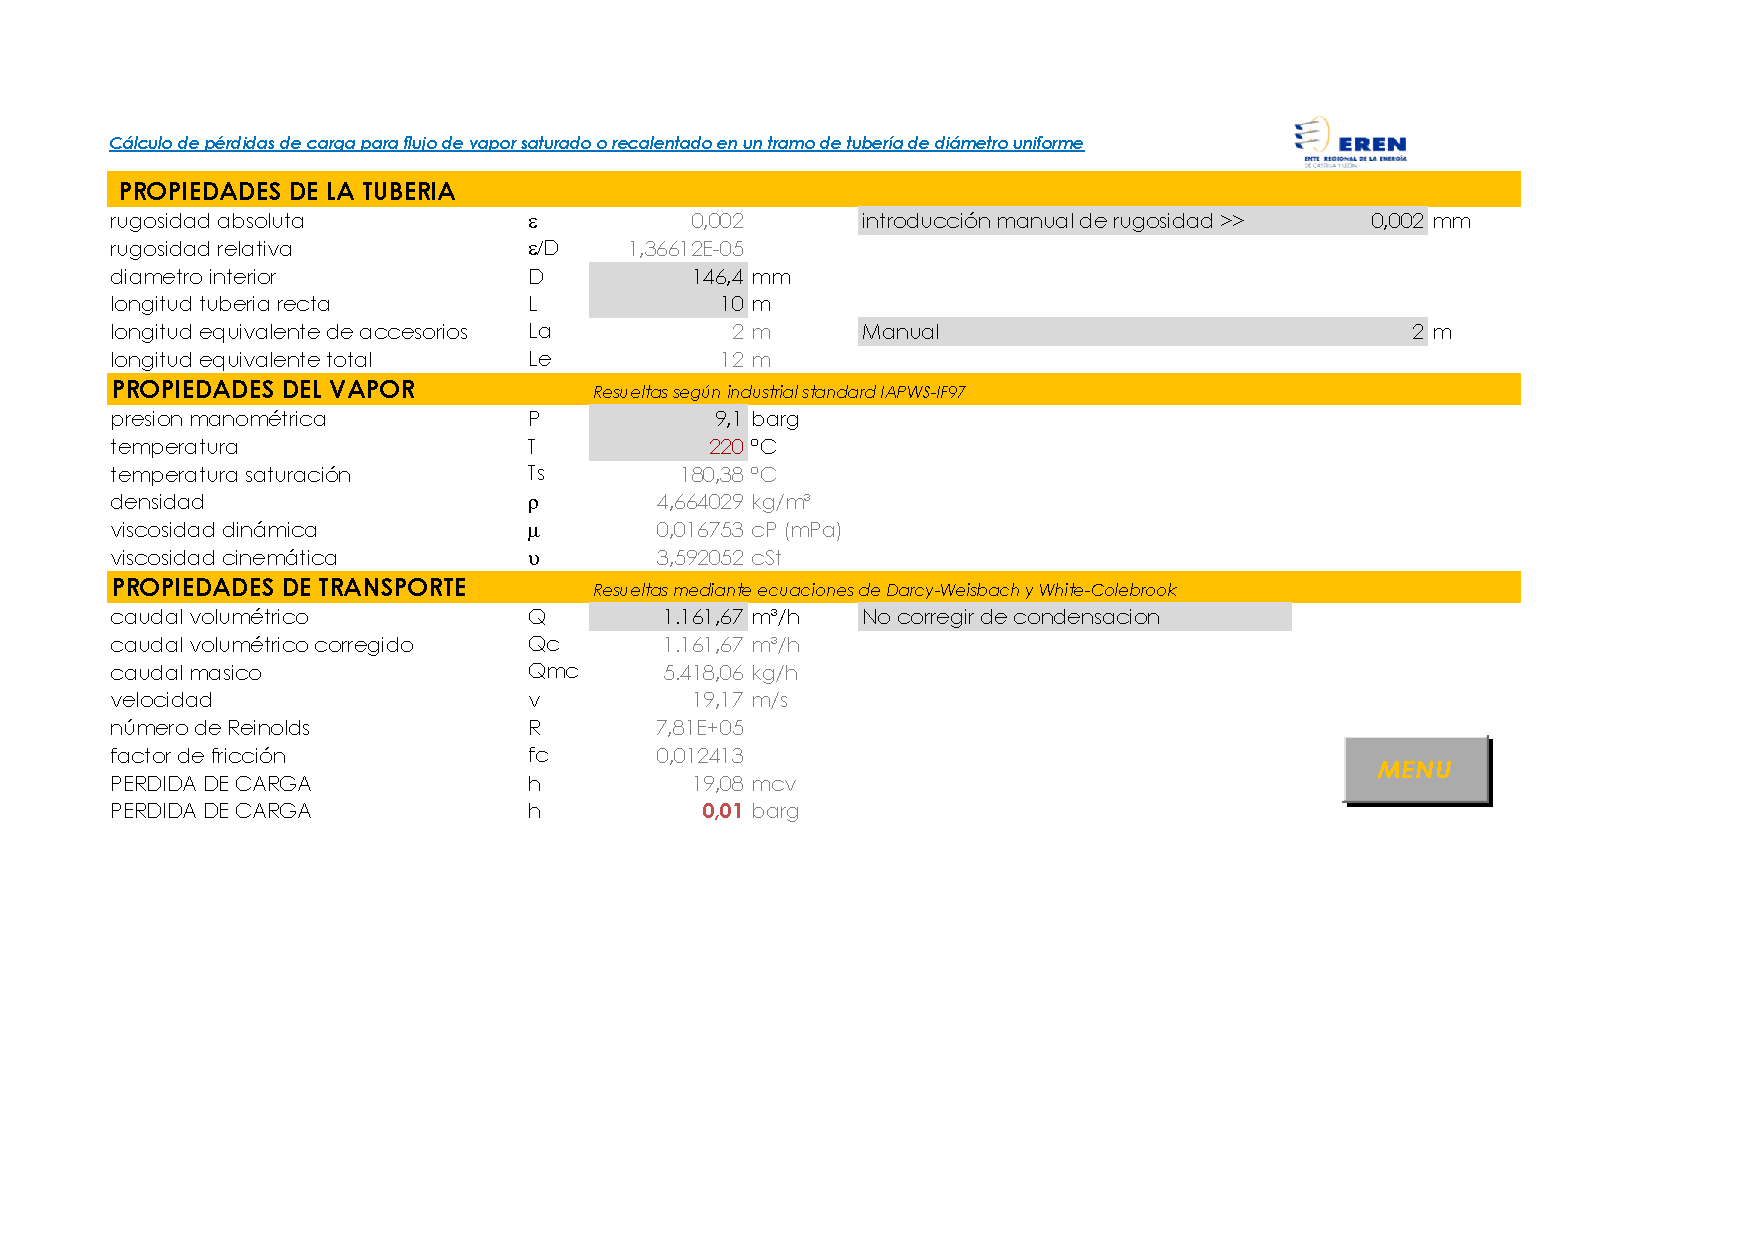
\includegraphics[trim={1cm 6cm 4cm 2cm}, clip, width=\textwidth]{Figuras/calculos_tramos/Vapor_TR1_Caldera-P.pdf}
	\caption{Hoja de cálculo del Tramo 1 (Caldera-P). Fuente: Elaboración grupal. \textit{Nota: Esta hoja de cálculo también se incluye completa en la \autoref{fig:anejo3-vapor-tr1} del \anexoref{anexo:calculos} para referencia detallada.}}
	\label{fig:hoja-calculo-tramo1}
\end{figure}

El croquis del tramo con su trazado y puntos característicos se presenta en la \figref{fig:croquis-tramo1}.

\begin{figure}[H]
	\centering
	
\includegraphics[trim = {2cm  6cm 2cm 5cm }, clip, width=0.6\textwidth]{Figuras/dibujos_tramos/Vapor_TR1_Caldera-P.pdf}
	\caption{Croquis del Tramo 1 (Caldera-P). Fuente: Elaboración grupal. \textit{Nota: Este diagrama también se incluye en la \autoref{fig:anejo2-vapor-tr1} del \anexoref{anexo:diagramas} para referencia detallada.}}
	\label{fig:croquis-tramo1}
\end{figure}

\subsubsection{Tramo 2: P-C1 (tramo enterrado)}
\label{subsubsec:tramo2-p-c1}

Este tramo conecta el punto de derivación P con el consumidor C1, constituyendo el tramo más largo de la instalación y el único con disposición enterrada. Esta configuración impone requisitos específicos tanto en la selección del material como en las condiciones de instalación.

\paragraph{Datos de partida}

Los datos geométricos y de servicio del tramo se recogen en la \tabref{tab:datos-tramo2}.

\begin{table}[H]
	\centering
	\caption{Datos de partida del Tramo 2 (P-C1). Fuente: Elaboración grupal.}
	\label{tab:datos-tramo2}
	\begin{tabular}{lc}
		\toprule
		\textbf{Parámetro}                    & \textbf{Valor}                 \\
		\midrule
		Longitud real (m)                     & 88{,}189                       \\
		Longitud equivalente (accesorios) (m) & 9{,}24                         \\
		Longitud de cálculo (m)               & 97{,}429                       \\
		Caudal másico (kg/h)                  & 1102{,}45                      \\
		Accesorios                            & 2 codos 90° + 1 T (paso recto) \\
		\bottomrule
	\end{tabular}
\end{table}

\paragraph{Tubería seleccionada}

Dada la condición de tramo enterrado, se selecciona una tubería con pared muy reforzada para garantizar la resistencia mecánica frente a las cargas del terreno y proporcionar mayor protección contra la corrosión por contacto con el suelo. Las características de la tubería se muestran en la \tabref{tab:tuberia-tramo2}.

\begin{table}[H]
	\centering
	\caption{Tubería seleccionada para el Tramo 2. Fuente: Elaboración grupal.}
	\label{tab:tuberia-tramo2}
	\begin{tabular}{lc}
		\toprule
		\textbf{Parámetro} & \textbf{Valor} \\
		\midrule
		Norma              & Schedule 160   \\
		Diámetro nominal   & DN~80          \\
		Diámetro interior  & 66{,}6         \\
		Diámetro exterior  & 88{,}9         \\
		\bottomrule
	\end{tabular}
\end{table}

La selección de Schedule 160 frente a alternativas de menor espesor (Schedule 40 o 80) se justifica por:
\begin{itemize}[noitemsep]
	\item Resistencia mecánica ante cargas verticales del terreno y posibles sobrecargas superficiales.
	\item Mayor margen de seguridad frente a corrosión exterior por contacto con el suelo.
	\item Compensación de posibles defectos de instalación en tramos de difícil inspección.
\end{itemize}

\paragraph{Verificación hidráulica}

Los resultados de la verificación hidráulica se presentan en la \tabref{tab:hidraulica-tramo2}. Este tramo presenta la mayor pérdida de carga de toda la red de vapor debido a su longitud.

\begin{table}[H]
	\centering
	\caption{Verificación hidráulica del Tramo 2. Fuente: Elaboración grupal.}
	\label{tab:hidraulica-tramo2}
	\begin{tabular}{lc}
		\toprule
		\textbf{Parámetro}          & \textbf{Valor} \\
		\midrule
		Velocidad real (m/s)        & 16{,}32        \\
		Pérdida de carga (bar)      & 0{,}18         \\
		Presión de entrada (bar(g)) & 9{,}058        \\
		Presión de salida (bar(g))  & 8{,}878        \\
		\bottomrule
	\end{tabular}
\end{table}

La velocidad de 16{,}32~m/s se encuentra dentro del rango admisible (15--30~m/s). La pérdida de carga de 0{,}18~bar resulta coherente con el caudal de diseño y la longitud de este tramo.

\paragraph{Condiciones de enterramiento}

Las condiciones de instalación del tramo enterrado se resumen en la \tabref{tab:enterramiento-tramo2}. El análisis térmico detallado de las pérdidas de calor al terreno se desarrolla en la \autoref{subsec:aislamiento_termico} dedicada al aislamiento térmico.

\begin{table}[H]
	\centering
	\caption{Condiciones de enterramiento del Tramo 2. Fuente: Elaboración grupal.}
	\label{tab:enterramiento-tramo2}
	\begin{tabular}{lc}
		\toprule
		\textbf{Parámetro}                 & \textbf{Valor}   \\
		\midrule
		Profundidad del eje de tubería (m) & 1{,}09           \\
		Profundidad total de zanja (m)     & 1{,}34           \\
		Ancho de zanja (m)                 & 1{,}50           \\
		Aislamiento térmico (mm)           & Lana de Roca, 50 \\
		\bottomrule
	\end{tabular}
\end{table}

\paragraph{Presión en el consumidor C1}

El consumidor C1 requiere una presión de trabajo de 4~bar(g) con un caudal de 679~kg/h. La presión disponible a la salida del tramo es de 8{,}878~bar(g), lo que proporciona un margen de +4{,}878~bar respecto a la presión requerida. Este exceso de presión se regulará mediante una válvula reductora de presión instalada en la acometida al consumidor.

\paragraph{Resultados}

En la \tabref{tab:resumen-tramo2} se presenta el resumen de resultados del dimensionado del Tramo 2.

\begin{table}[H]
	\centering
	\caption{Resumen de resultados del Tramo 2 (P-C1). Fuente: Elaboración grupal.}
	\label{tab:resumen-tramo2}
	\begin{tabular}{lc}
		\toprule
		\textbf{Parámetro}        & \textbf{Valor}        \\
		\midrule
		Tubería                   & Schedule 160 -- DN~80 \\
		Diámetro interior [mm]         & 66{,}6            \\
		Longitud total de cálculo [m] & 97{,}429           \\
		Caudal másico [kg/h]             & 1102{,}45       \\
		Velocidad [m/s]                 & 16{,}32          \\
		Pérdida de carga [bar]          & 0{,}18           \\
		Presión entrada [bar(g)]           & 9{,}058       \\
		Presión salida (C1) [bar(g)]       & 8{,}878      \\
		\bottomrule
	\end{tabular}
\end{table}

Los cálculos detallados de pérdida de carga se muestran en la \autoref{fig:anejo3-vapor-tr2} del \anexoref{anexo:calculos}, mientras que el esquema del tramo con sus cotas y accesorios se presenta en la \autoref{fig:anejo2-vapor-tr2} del \anexoref{anexo:diagramas}.

\subsubsection{Tramo 3: P-S}
\label{subsubsec:tramo3-p-s}

El tramo P-S constituye la línea principal que alimenta a los consumidores C2, C3 y C4, transportando el caudal combinado de estos tres puntos de consumo.

\paragraph{Datos de partida}

El tramo P-S tiene una longitud real de 106~m, con una longitud equivalente de 25,44~m debida a los accesorios (1 codo 90° + 2 T en derivación), resultando en una longitud de cálculo de 131,44~m.

La obtenci\'on del caudal m\'asico se desarrolla como suma de demandas aguas abajo:

\begin{equation}
	\dot{m}_{\text{TR3}} = 4619{,}15~\text{kg/h}
	\label{eq:caudal-tramo3}
\end{equation}

\paragraph{Tubería seleccionada}

Se ha seleccionado tubería DN~125 según norma DIN 2448, con diámetro interior de 131,7~mm.

\paragraph{Verificación hidráulica}

La velocidad resultante es de 25,06~m/s, dentro del rango admisible de diseño. La pérdida de carga es de 0,23~bar, con presión de entrada de 9,058~bar(g) y presión de salida de 8,83~bar(g). Los resultados completos del dimensionado se presentan en la \tabref{tab:resumen-red-vapor}. Los cálculos detallados se muestran en la \autoref{fig:anejo3-vapor-tr3} del \anexoref{anexo:calculos}, y el esquema del tramo en la \autoref{fig:anejo2-vapor-tr3} del \anexoref{anexo:diagramas}.

\subsubsection{Tramo 4: S-C2}
\label{subsubsec:tramo4-s-c2}

Este tramo conecta el nodo S con el consumidor C2, siendo un tramo relativamente corto y sin accesorios significativos.

\paragraph{Datos de partida}

El tramo tiene una longitud real de 25~m, siendo un tramo relativamente corto y sin accesorios significativos. La longitud equivalente se estima como el 20\% de la longitud real (5~m), resultando en una longitud de cálculo de 30~m.

El caudal másico de diseño del tramo se obtiene como:

\begin{equation}
	\dot{m}_{\text{TR4}} = 1884{,}45~\text{kg/h}
	\label{eq:caudal-tramo4}
\end{equation}

\paragraph{Tubería seleccionada}

Se ha seleccionado tubería DN~80 según norma DIN 2448, con diámetro interior de 82,5~mm.

\paragraph{Verificación hidráulica}

La velocidad resultante es de 29,74~m/s, situándose en el límite superior del criterio de velocidad máxima admisible (30 m/s). La pérdida de carga es de 0,13~bar. Con presión de entrada de 8,83~bar(g), la presión de salida es de 8,70~bar(g), superando ampliamente la presión requerida por C2 (7~bar(g)) y proporcionando un margen de 1,70~bar. Los resultados completos del dimensionado se presentan en la \tabref{tab:resumen-red-vapor}. Los cálculos detallados se muestran en la \autoref{fig:anejo3-vapor-tr4} del \anexoref{anexo:calculos}, y el esquema del tramo en la \autoref{fig:anejo2-vapor-tr4} del \anexoref{anexo:diagramas}.

\subsubsection{Tramos 5, 6 y 7: rama S-T-C3-C4}
\label{subsubsec:tramos5-6-7}

Los tramos 5, 6 y 7 conforman la rama que alimenta a los consumidores C3 y C4, partiendo del nodo S. El nodo T actúa como punto de bifurcación hacia estos dos consumidores.

\paragraph{Tramo 5: S-T}

La obtenci\'on del caudal m\'asico del tramo se realiza como:

\begin{equation}
	\dot{m}_{\text{TR5}} = 3056{,}3~\text{kg/h}
	\label{eq:caudal-tramo5}
\end{equation}

El tramo S-T transporta este caudal combinado. Tiene una longitud real de 60~m, con accesorios que incluyen 1 T en configuración recta y 1 T en derivación, totalizando una longitud de cálculo de 78~m. Se ha seleccionado tubería DIN 2448 -- DN~100 (diámetro interior 107,1~mm), resultando en una velocidad de 26,73~m/s y una pérdida de carga de 0,19~bar. Los resultados completos del dimensionado se presentan en la \tabref{tab:resumen-red-vapor}.

\paragraph{Tramo 6: T-C3}

La obtenci\'on del caudal m\'asico del tramo se realiza como:

\begin{equation}
	\dot{m}_{\text{TR6}} = 712{,}6~\text{kg/h}
	\label{eq:caudal-tramo6}
\end{equation}

Este tramo alimenta al consumidor C3, siendo el de menor caudal de la instalación. Es un tramo corto con longitud real de 15~m y longitud de cálculo de 18~m. Se ha seleccionado tubería Schedule 40 -- DN~50 (diámetro interior 52,5~mm), resultando en una velocidad de 28,15~m/s y una pérdida de carga de 0,12~bar. Los resultados completos del dimensionado se presentan en la \tabref{tab:resumen-red-vapor}.

\paragraph{Tramo 7: T-C4}

La obtenci\'on del caudal m\'asico del tramo se realiza como:

\begin{equation}
	\dot{m}_{\text{TR7}} = 2665{,}3~\text{kg/h}
	\label{eq:caudal-tramo7}
\end{equation}

El tramo T-C4 alimenta al consumidor de mayor caudal de la instalación. Tiene una longitud real de 45~m, con accesorios que incluyen 2 codos de 90° y 1 T en configuración recta, totalizando una longitud de cálculo de 57,4~m. Se ha seleccionado tubería Schedule 40 -- DN~100 (diámetro interior 102,3~mm), resultando en una velocidad de 26,29~m/s y una pérdida de carga de 0,14~bar. Los resultados completos del dimensionado se presentan en la \tabref{tab:resumen-red-vapor}.

Los tres tramos mantienen velocidades muy próximas al objetivo de diseño (20~m/s), confirmando la coherencia del dimensionado. Las hojas de cálculo detalladas se presentan en las Figuras del \anexoref{anexo:calculos}, y los esquemas correspondientes en las  del \anexoref{anexo:diagramas}.

\subsubsection{Resumen de la red de vapor}
\label{subsubsec:resumen-red-vapor}

El dimensionado hidráulico de cada tramo se ha calculado y verificado asegurando que se cumplen los criterios de diseño hidráulico en la red de distribución. En la \tabref{tab:resumen-red-vapor} se presenta el resumen consolidado de los parámetros de diseño para cada tramo.

\begin{table}[H]
	\centering
	\small
	\caption{Resumen del dimensionado hidráulico de la red de vapor. Fuente: Elaboración grupal.}
	\label{tab:resumen-red-vapor}
	\resizebox{\textwidth}{!}{
		\begin{tabular}{lcccccc}
			\toprule
			\textbf{Tramo}  & \textbf{Tubería} & \textbf{DN} & \textbf{Caudal [kg/h]} & \textbf{Velocidad [m/s]} & \textbf{$\Delta P$ [bar]} \\
			\midrule
			TR1 (Caldera-P) & Schedule 80      & 150         & 5400,00                & 19,17                    & 0,01                      \\
			TR2 (P-C1)      & Schedule 160     & 80          & 1102,45                & 16,32                    & 0,18                      \\
			TR3 (P-S)       & DIN 2448         & 125         & 4619,15                & 25,06                    & 0,23                      \\
			TR4 (S-C2)   & DIN 2448         & 80          & 1884,45                & 29,74                    & 0,13                      \\
			TR5 (S-T)       & DIN 2448         & 100         & 3056,30                & 26,73                    & 0,19                      \\
			TR6 (T-C3)   & Schedule 40      & 50          & 712,60                 & 28,15                    & 0,12                      \\
			TR7 (T-C4)   & Schedule 40      & 100         & 2665,30                & 26,29                    & 0,14                      \\
			\bottomrule
		\end{tabular}
	}
\end{table}

A continuación se presentan las tablas de verificación general del dimensionado de la red de vapor aisladas en formato apaisado, permitiendo validar los accesorios, presiones y pérdidas acumuladas.

\begin{landscape}
	\begin{table}[H]
		\centering
		\small
		\caption{Tablas de verificación del dimensionado hidráulico de la red de vapor. Fuente: Elaboración grupal.}
		\label{tab:verificacion-red-vapor-completa}

		\begin{minipage}{\linewidth}
			\centering
			\textbf{1. Accesorios por tramo y cálculo de longitudes equivalentes}
			\vspace{0.2cm}
			\begin{tabular}{lcccccccc}
				\toprule
				\textbf{Tramo} & \textbf{$L_{real}$ (m)} & \textbf{Codos} & \textbf{T (recta)} & \textbf{T (deriv.)} & \textbf{$D_{tanteo}$ (mm)} & \textbf{$L_{eq}$ (m)} & \textbf{$L_{calc}$ (m)} \\
				\midrule
				Caldera-P      & 12,74                   & 0              & 0                  & 0                   & ---                        & 2,55                  & 15,29                   \\
				P-C1           & 88,19                   & 2              & 1                  & 0                   & 60                         & 9,24                  & 97,43                   \\
				P-S            & 106,00                  & 1              & 0                  & 2                   & 120                        & 25,44                 & 131,44                  \\
				S-C2        & 25,00                   & 0              & 0                  & 0                   & ---                        & 5,00                  & 30,00                   \\
				S-T            & 60,00                   & 0              & 1                  & 1                   & 120                        & 7,50                  & 78,00                   \\
				T-C3        & 15,00                   & 0              & 0                  & 0                   & ---                        & 3,00                  & 18,00                   \\
				T-C4        & 45,00                   & 2              & 1                  & 0                   & 100                        & 12,40                 & 57,40                   \\
				\bottomrule
			\end{tabular}
		\end{minipage}

		\vspace{1.5cm}

		\begin{minipage}{0.48\linewidth}
			\centering
			\textbf{2. Presiones en los consumidores de vapor}
			\vspace{0.2cm}
			\begin{tabular}{lccc}
				\toprule
				\textbf{Consumidor} & \textbf{$P_{disponible}$ [bar(g)]} & \textbf{$P_{requerida}$ [bar(g)]} & \textbf{Margen [bar]} \\
				\midrule
				C1                  & 8,878                              & 4,0                               & +4,878                \\
				C2               & 8,698                              & 7,0                               & +1,698                \\
				C3               & 8,518                              & 7,0                               & +1,518                \\
				C4               & 8,498                              & 7,0                               & +1,498                \\
				\bottomrule
			\end{tabular}
		\end{minipage}
		\hfill
		\begin{minipage}{0.48\linewidth}
			\centering
			\textbf{3. Pérdida de carga acumulada en la red de vapor}
			\vspace{0.2cm}
			\begin{tabular}{llc}
				\toprule
				\textbf{Consumidor} & \textbf{Ruta de suministro}                                                 & \textbf{$\Delta P_{total}$ [bar]} \\
				\midrule
				C1                  & Caldera $\rightarrow$ P $\rightarrow$ C1                                    & 0,19                              \\
				C2               & Caldera $\rightarrow$ P $\rightarrow$ S $\rightarrow$ C2                 & 0,37                              \\
				C3               & Caldera $\rightarrow$ P $\rightarrow$ S $\rightarrow$ T $\rightarrow$ C3 & 0,55                              \\
				C4               & Caldera $\rightarrow$ P $\rightarrow$ S $\rightarrow$ T $\rightarrow$ C4 & 0,57                              \\
				\bottomrule
			\end{tabular}
		\end{minipage}
	\end{table}
\end{landscape}


El dimensionado hidráulico de la red de vapor cumple satisfactoriamente con todos los criterios de diseño establecidos:

\begin{itemize}[noitemsep]
	\item Todas las velocidades se mantienen en el rango 16{,}32--29{,}74~m/s, cumpliendo con el límite de 30 m/s.
	\item La pérdida de carga total máxima (0{,}57~bar hasta C4) es inferior al criterio de 1~bar.
	\item Todos los consumidores disponen de presión suficiente con márgenes adecuados.
	\item El consumidor C1 requiere válvula reductora debido a su menor presión de trabajo (4~bar(g)).
\end{itemize}

\subsection{Dimensionado Hidráulico de la Red de Condensados}
\label{subsec:dimensionado-condensados}

La red de retorno de condensados constituye un elemento fundamental para la eficiencia energética de la instalación. El condensado generado en los consumidores retorna a la caldera mediante una red presurizada, aprovechando tanto la energía térmica residual del líquido como el vapor de revaporizado (vapor flash) generado en el proceso de expansión.

El diseño de esta red presenta particularidades respecto a la red de vapor, debido a la presencia de flujo bifásico (líquido + vapor flash) que requiere criterios de velocidad específicos y consideraciones adicionales de dimensionado.

\subsubsection{Consideraciones sobre Retorno de Condensados y Vapor Flash}
\label{subsubsec:consideraciones-condensados}

Cuando el condensado a alta presión (9~bar(g) en los consumidores) pasa a través del purgador y entra en la línea de retorno a menor presión, parte del condensado se revaporiza produciendo el denominado \textit{vapor flash} o \textit{vapor de revaporizado}. Este fenómeno se debe al exceso de entalpía del líquido respecto a las condiciones de saturación a la nueva presión.

\paragraph{Presión de diseño de la red de condensados}

La presión de diseño de la red de retorno se establece según el criterio:

\begin{equation}
	P_{red} = P_{min,consumidor} - 1~\text{bar} = 4 - 1 = 3~\text{bar(g)}
	\label{eq:presion-red-condensados}
\end{equation}

donde $P_{min,consumidor}$ corresponde a la presión mínima de trabajo entre todos los consumidores, en este caso el consumidor C1 con 4~bar(g).

\paragraph{Características del flujo bifásico}

El vapor flash presenta un volumen específico significativamente mayor que el líquido, lo que determina las características del flujo en la tubería:

\begin{itemize}[noitemsep]
	\item Relación volumétrica aproximada: 98\% vapor, 2\% líquido
	\item Velocidad de diseño para flujo bifásico: 15--20~m/s (superior al condensado puro)
	\item El vapor flash representa energía recuperable aprovechable
\end{itemize}

\paragraph{Opciones de aprovechamiento del vapor flash}

El vapor de revaporizado puede aprovecharse mediante diferentes estrategias:

\begin{enumerate}[noitemsep]
	\item Tanques de revaporizado para separación de fases
	\item Inyección directa en procesos de baja presión
	\item Precalentamiento del agua de alimentación a la caldera
\end{enumerate}

\subsubsection{Cálculo del Porcentaje de Vapor Flash}
\label{subsubsec:calculo-vapor-flash}

El porcentaje de vapor flash generado se determina mediante un balance entálpico entre las condiciones de entrada (presión del consumidor) y las condiciones de la red de retorno.

\paragraph{Ecuación del balance entálpico}

\begin{equation}
	\%v_f = \frac{h_{lp1} - h_{lp2}}{h_{vp2} - h_{lp2}} \times 100
	\label{eq:vapor-flash}
\end{equation}

donde:
\begin{itemize}[noitemsep]
	\item $h_{lp1}$ = entalpía del líquido saturado a la presión del consumidor
	\item $h_{lp2}$ = entalpía del líquido saturado a la presión de la red de retorno
	\item $h_{vp2}$ = entalpía del vapor saturado a la presión de la red de retorno
\end{itemize}

\paragraph{Datos termodinámicos}

Los valores de entalpía se obtienen de las tablas de vapor saturado para las condiciones de operación:

\begin{table}[H]
	\centering
	\caption{Propiedades termodinámicas para el cálculo del vapor flash}
	\label{tab:propiedades-flash}
	\begin{tabular}{lcc}
		\toprule
		\textbf{Parámetro}                 & \textbf{Símbolo} & \textbf{Valor} \\
		\midrule
		Presión consumidor (bar(g))        & $P_1$            & 9              \\
		Presión red retorno (bar(g))       & $P_2$            & 3              \\
		Entalpía líq. sat. a $P_1$ (kJ/kg) & $h_{l,P_1}$      & 763{,}05       \\
		Entalpía líq. sat. a $P_2$ (kJ/kg) & $h_{l,P_2}$      & 604{,}67       \\
		Entalpía vap. sat. a $P_2$ (kJ/kg) & $h_{v,P_2}$      & 2738{,}09     \\
		\bottomrule
	\end{tabular}
\end{table}

\paragraph{Cálculo del porcentaje de vapor flash}

Sustituyendo los valores en la \autoref{eq:vapor-flash}:

\begin{equation}
	\begin{split}
		\%v_f & = \frac{763{,}05 - 604{,}67}{2738{,}09 - 604{,}67} \times 100 \\
		      & = \frac{158{,}38}{2133{,}42} \times 100 = 7{,}45\%
	\end{split}
	\label{eq:vapor-flash-resultado}
\end{equation}

\paragraph{Caudales resultantes}

A partir del caudal total de condensado y el porcentaje de vapor flash calculado, se determinan los caudales de cada fase:

\begin{table}[H]
	\centering
	\caption{Distribución de caudales en la red de condensados}
	\label{tab:caudales-condensados}
	\begin{tabular}{lc}
		\toprule
		\textbf{Componente}    & \textbf{Caudal (kg/h)} \\
		\midrule
		Condensado total       & 5403{,}95             \\
		Vapor flash (7{,}45\%) & 402{,}54               \\
		Condensado líquido     & 5001{,}41             \\
		\bottomrule
	\end{tabular}
\end{table}


\subsubsection{Dimensionado de los Tramos de Condensados}
\label{subsubsec:dimensionado-tramos-condensados}

La red de condensados consta de 7 segmentos que conectan los consumidores con el colector de retorno a la caldera. Todos los tramos utilizan tubería de acero Schedule~40, que ofrece mayor resistencia a la corrosión por CO$_2$ disuelto en el condensado.

El material de todas las tuberías es acero al carbono Schedule 40, con diámetros seleccionados para mantener velocidades de diseño entre 15 y 20~m/s.


\subsubsection{Resumen de la Red de Condensados}
\label{subsubsec:resumen-condensados}

El dimensionamiento hidráulico se integra en el diseño de la red de condensados como se muestra en la \tabref{tab:resumen-red-condensados}. En todos los casos se respetan los límites de velocidad admisible para el transporte en régimen bifásico sin riesgo de severa erosión.

\begin{table}[H]
	\centering
	\normalsize
	\caption{Resumen del dimensionado hidráulico de la red de condensados. Fuente: Elaboración grupal.}
	\label{tab:resumen-red-condensados}
	\begin{tabular}{lccccc}
		\toprule
		\textbf{Tramo}  & \textbf{DN} & \textbf{Caudal [kg/h]} & \textbf{Velocidad [m/s]} & \textbf{$\Delta P$ [bar]} \\
		\midrule
		TR1 (Caldera-P) & 65          & 5400,00                & 19,31                    & 0,02                      \\
		TR2 (P-C1)      & 32          & 1102,45                & 17,78                    & 0,25                      \\
		TR3 (P-S)       & 65          & 4619,15                & 19,13                    & 0,14                      \\
		TR4 (S-C2)   & 50          & 1884,45                & 18,04                    & 0,05                      \\
		TR5 (S-T)       & 65          & 3056,30                & 17,70                    & 0,08                      \\
		TR6 (T-C3)   & 25          & 712,60                 & 17,96                    & 0,05                      \\
		TR7 (T-C4)   & 50          & 2665,30                & 17,41                    & 0,06                      \\
		\bottomrule
	\end{tabular}
\end{table}


A continuación se exponen las tablas de verificación aisladas en formato apaisado, detallando los accesorios de la red, las presiones disponibles respecto a las exigidas, y la caída de presión acumulada desde los consumidores hasta el punto de recolección en caldera.

\begin{landscape}
	\begin{table}[H]
		\centering
		\normalsize
		\caption{Tablas de verificación del dimensionado hidráulico de la red de condensados. Fuente: Elaboración grupal.}
		\label{tab:verificacion-red-condensados-completa}

		\begin{minipage}{\linewidth}
			\centering
			\textbf{1. Accesorios por tramo y cálculo de longitudes equivalentes}
			\vspace{0.2cm}
			\begin{tabular}{lcccccccc}
				\toprule
				\textbf{Tramo} & \textbf{$L_{real}$ (m)} & \textbf{Codos} & \textbf{T (recta)} & \textbf{T (deriv.)} & \textbf{$D_{tanteo}$ (mm)} & \textbf{$L_{eq}$ (m)} & \textbf{$L_{calc}$ (m)} \\
				\midrule
				Caldera-P      & 12,74                   & 0              & 0                  & 0                   & ---                        & 2,55                  & 15,29                   \\
				P-C1           & 61,87                   & 2              & 1                  & 0                   & 40                         & 6,16                  & 68,03                   \\
				P-S            & 105,00                  & 1              & 0                  & 2                   & 60                        & 13,78                 & 118,78                  \\
				S-C2        & 24,00                   & 0              & 0                  & 0                   & ---                        & 4,80                  & 28,80                   \\
				S-T            & 60,00                   & 0              & 1                  & 1                   & 50                         & 5,50                  & 65,50                   \\
				T-C3        & 14,00                   & 0              & 0                  & 0                   & ---                        & 2,80                  & 16,80                   \\
				T-C4        & 44,00                   & 2              & 1                  & 0                   & 50                         & 6,20                  & 50,20                   \\
				\bottomrule
			\end{tabular}
		\end{minipage}

		\vspace{1.5cm}

		\begin{minipage}{0.48\linewidth}
			\centering
			\textbf{2. Presiones en los puntos de recolección de condensados}
			\vspace{0.2cm}
			\begin{tabular}{lccc}
				\toprule
				\textbf{Consumidor} & \textbf{$P_{disponible}$ [bar(g)]} & \textbf{$P_{requerida}$ [bar(g)]} & \textbf{Estado} \\
				\midrule
				C1                  & 2,73                               & 3,0                               & Operativa       \\
				C2               & 2,82                               & 3,0                               & Operativa       \\
				C3               & 2,70                               & 3,0                               & Operativa       \\
				C4               & 2,71                               & 3,0                               & Operativa       \\
				\bottomrule
			\end{tabular}
		\end{minipage}
		\hfill
		\begin{minipage}{0.48\linewidth}
			\centering
			\textbf{3. Pérdida de carga acumulada en la red de condensados}
			\vspace{0.2cm}
			\begin{tabular}{llc}
				\toprule
				\textbf{Consumidor} & \textbf{Ruta de retorno}                                                & \textbf{$\Delta P_{total}$ [bar]} \\
				\midrule
				C1                  & Caldera $\leftarrow$ P $\leftarrow$ C1                                  & 0,27                              \\
				C2               & Caldera $\leftarrow$ P $\leftarrow$ S $\leftarrow$ C2                & 0,18                              \\
				C3               & Caldera $\leftarrow$ P $\leftarrow$ S $\leftarrow$ T $\leftarrow$ C3 & 0,30                              \\
				C4               & Caldera $\leftarrow$ P $\leftarrow$ S $\leftarrow$ T $\leftarrow$ C4 & 0,29                              \\
				\bottomrule
			\end{tabular}
		\end{minipage}
	\end{table}
\end{landscape}


El dimensionado hidráulico de la red de condensados cumple satisfactoriamente con todos los criterios de diseño establecidos:

\begin{itemize}[noitemsep]
	\item Todas las velocidades se mantienen en el rango 17{,}41--19{,}31~m/s, dentro del criterio de 15--20~m/s para flujo bifásico.
	\item La pérdida de carga máxima acumulada (0{,}30~bar hasta C3) es aceptable para la presión de operación de 3~bar(g).
	\item El porcentaje de vapor flash calculado (7{,}45\%) justifica el uso de criterios de flujo bifásico.
\end{itemize}


\subsection{Aislamiento Térmico y Detalles de Instalación}
\label{subsec:aislamiento_termico}

El diseño del aislamiento térmico constituye un aspecto fundamental en la eficiencia energética, seguridad operacional y viabilidad económica de instalaciones de vapor. Un aislamiento adecuado minimiza las pérdidas térmicas hacia el ambiente, protege al personal de superficies calientes, previene la condensación prematura del vapor en las tuberías y reduce los costes operativos del sistema. Esta subsección desarrolla el dimensionado completo del aislamiento térmico para la red de distribución, tanto en tramos aéreos como en el tramo enterrado, aplicando criterios normativos y buenas prácticas de ingeniería.


\subsubsection{Criterios de Aislamiento Térmico}
\label{subsubsec:criterios_aislamiento}

El dimensionado del aislamiento térmico debe satisfacer simultáneamente tres objetivos:

\begin{enumerate}[noitemsep]
	\item Eficiencia energética: Minimizar las pérdidas térmicas durante el transporte de vapor y condensados.
	\item Seguridad del personal: Limitar la temperatura superficial del aislamiento para evitar riesgos de quemaduras en zonas accesibles.
	\item Viabilidad económica: Optimizar el espesor para equilibrar coste de inversión con ahorros energéticos.
\end{enumerate}

\paragraph{Condiciones de operación y ambientales}
\label{par:condiciones_operacion_aisl}

Las temperaturas de operación de los fluidos en la instalación son:

\begin{itemize}[noitemsep]
	\item Red de vapor: $T_{\text{vap}} = 220$~°C (vapor saturado a 21~bar(g)).
	\item Red de condensados: $T_{\text{cond}} = 143{,}6$~°C (condensado saturado a 3~bar(g)).
\end{itemize}

Las condiciones ambientales adoptadas para el cálculo son:

\begin{itemize}[noitemsep]
	\item Ambiente exterior (tramos aéreos): $T_{\text{amb}} = 15$~°C, coeficiente convectivo $h_{\text{ext}} = 25$~W/(m$^2\cdot$K).
	\item Terreno (tramo enterrado): $T_{\text{terr}} = 10$~°C, conductividad térmica $\lambda_{\text{terr}} = 1{,}2$~W/(m$\cdot$K).
\end{itemize}

\paragraph{Materiales seleccionados}
\label{par:materiales_aislamiento}

Los materiales considerados en el cálculo térmico son:

\begin{itemize}[noitemsep]
	\item Aislamiento térmic: Lana de roca de alta densidad (120--150~kg/m$^3$), con conductividad térmica $\lambda_{\text{aisl}} = 0{,}04$~W/(m$\cdot$K) a temperatura media. Este material es ampliamente utilizado en instalaciones industriales por su excelente resistencia térmica, estabilidad dimensional a altas temperaturas y propiedades ignífugas.
	\item Tubería: Acero al carbono, con conductividad térmica $\lambda_{\text{acero}} = 50$~W/(m$\cdot$K).
\end{itemize}

\paragraph{Criterio normativo: RITE (RD 1027/2007)}
\label{par:criterio_rite}

El Reglamento de Instalaciones Térmicas en los Edificios (RITE) \cite{RITE2007} establece como criterio de seguridad que la temperatura superficial del aislamiento en zonas accesibles no supere los 30~°C, con el objetivo de eliminar el riesgo de quemaduras por contacto accidental. Este criterio se adopta como referencia para el dimensionado del espesor de aislamiento en tramos aéreos.

\paragraph{Modelo de transferencia de calor}
\label{par:modelo_transferencia}

El flujo de calor por unidad de longitud desde el fluido hacia el ambiente se calcula mediante la ecuación general de resistencias térmicas en serie:

\begin{equation}
	q_L = \frac{\Delta T}{\sum R}
	\label{eq:perdida_lineal_aisl}
\end{equation}

\noindent donde $\Delta T$ es la diferencia de temperatura entre el fluido y el ambiente, y $\sum R$ es la resistencia térmica total del sistema por unidad de longitud.

Las resistencias térmicas de cada capa cilíndrica se expresan mediante las siguientes ecuaciones:

\begin{equation}
	R_{\text{pipe}} = \frac{\ln(r_1 / r_{\text{int}})}{2\pi \lambda_{\text{acero}}}
	\label{eq:resist_tuberia}
\end{equation}

\begin{equation}
	R_{\text{aisl}} = \frac{\ln(r_2 / r_1)}{2\pi \lambda_{\text{aisl}}}
	\label{eq:resist_aislamiento}
\end{equation}

\begin{equation}
	R_{\text{surf}} = \frac{1}{\pi d_e h_{\text{ext}}}
	\label{eq:resist_superficie}
\end{equation}

\noindent donde $r_{\text{int}}$ es el radio interior de la tubería, $r_1$ es el radio exterior de la tubería, $r_2$ es el radio exterior del aislamiento, y $d_e = 2r_2$ es el diámetro exterior del conjunto aislado.

Para tramos enterrados, se añade la resistencia térmica del terreno, modelada mediante la ecuación de cilindro enterrado:

\begin{equation}
	R_{\text{terr}} = \frac{\ln(2 h_{\text{eje}} / r_2)}{2\pi \lambda_{\text{terr}}}
	\label{eq:resist_terreno}
\end{equation}

\noindent donde $h_{\text{eje}}$ es la profundidad del eje de la tubería respecto a la superficie del terreno. Adicionalmente, la resistencia térmica de la canalización (arena envolvente) se estima como $R_{\text{can}} \approx 0{,}05$~m$\cdot$K/W, valor típico para lechos de arena compactada.

Es importante destacar que, debido a la baja conductividad térmica del material aislante ($\lambda_{\text{aisl}} = 0{,}04$~W/(m$\cdot$K)), la resistencia del aislamiento $R_{\text{aisl}}$ es la resistencia dominante del sistema, representando típicamente más del 85\% de la resistencia térmica total. Las resistencias de la pared metálica ($R_{\text{pipe}}$) y de la superficie exterior ($R_{\text{surf}}$) tienen contribuciones menores pero no despreciables.


\subsubsection{Aislamiento de Tuberías Aéreas}
\label{subsubsec:aislamiento_aereo}

El diseño del aislamiento para los tramos aéreos de la instalación se basa en criterios de estandarización que permiten agrupar tuberías de diámetros nominales similares en rangos con espesor de aislamiento común. Esta estrategia, recomendada por guías de eficiencia energética (IDAE \cite{IDAE2007}, ISO 12241 \cite{ISO12241}) y fabricantes especializados (Isover, Spirax Sarco \cite{SpiraxSarco2020}), presenta múltiples ventajas:

\begin{itemize}[noitemsep]
	\item Reducción de costes logísticos: Menor variedad de productos a adquirir y almacenar.
	\item Simplificación de inventario: Facilita la gestión de materiales en obra y mantenimiento.
	\item Facilidad de instalación: Los operarios trabajan con un número limitado de espesores estándar.
	\item Mantenimiento predictivo: La estandarización facilita la reposición de tramos dañados.
\end{itemize}

\paragraph{Criterios de estandarización por rangos de DN}
\label{par:rangos_estandarizados}

Los espesores de aislamiento seleccionados para la instalación, agrupados por rangos de diámetro nominal y tipo de red, se presentan en la \tabref{tab:rangos_estandarizados}.

\begin{table}[htbp]
	\centering
	\caption{Espesores de aislamiento estandarizados por rango de DN y tipo de red.}
	\label{tab:rangos_estandarizados}
	\begin{tabular}{lccc}
		\toprule
		\textbf{Red}             & \textbf{Rango DN (mm)} & \textbf{Espesor aislamiento (mm)} \\
		\midrule
		Vapor (220~°C)           & DN $\geq$ 125          & 100                               \\
		                         & DN 50--100             & 80                                \\
		                         & DN $<$ 50              & 60                                \\
		\midrule
		Condensados (143{,}6~°C) & DN $\geq$ 50           & 50                                \\
		                         & DN $<$ 50              & 40                                \\
		\bottomrule
	\end{tabular}
\end{table}

Estos espesores han sido verificados mediante cálculo térmico iterativo para garantizar el cumplimiento del criterio RITE ($T_{\text{surf}} \leq 30$~°C) en todos los tramos aéreos, con un margen de seguridad adecuado.

\paragraph{Resultados del dimensionado: Red de vapor}
\label{par:resultados_vapor_aereo}

La \tabref{tab:aislamiento_vapor_aereo} presenta el resumen completo del aislamiento térmico para los tramos aéreos de la red de vapor. Los cálculos se realizaron aplicando las ecuaciones \eqref{eq:perdida_lineal_aisl} a \eqref{eq:resist_superficie}, con las resistencias térmicas calculadas para cada diámetro y espesor de aislamiento.

\begin{table}[H]
	\centering
	\normalsize
	\setlength{\tabcolsep}{3pt}
	\caption{Dimensionado de aislamiento térmico para tramos aéreos de la red de vapor.}
	\label{tab:aislamiento_vapor_aereo}
	\begin{tabular}{lcccccc}
		\toprule
		\textbf{Tramo}           & \textbf{DN (mm)} & \textbf{$L$ (m)}  & \textbf{$e_{\text{aisl}}$ (mm)} & \textbf{$q_L$ (W/m)} & \textbf{$Q$ (W)} \\
		\midrule
		TR1 (Caldera--P)         & 150              & 12{,}74           & 100                             & 65{,}1               & 829              \\
		TR3 (P--S)               & 125              & 106{,}00          & 100                             & 57{,}9               & 6\,137           \\
		TR4 (S--C2)           & 80               & 25{,}00           & 80                              & 49{,}4               & 1\,235           \\
		TR5 (S--T)               & 100              & 60{,}00           & 80                              & 58{,}1               & 3\,486           \\
		TR6 (T--C3)           & 50               & 15{,}00           & 80                              & 39{,}3               & 590              \\
		TR7 (T--C4)           & 100              & 45{,}00           & 80                              & 58{,}1               & 2\,615           \\
		\midrule
		\textbf{TOTAL RED VAPOR} & ---              & \textbf{263{,}74} & ---                             & ---                  & \textbf{14\,892} \\
		\bottomrule
	\end{tabular}
	
	\vspace{0.3cm}

	\noindent \small \textit{Nota}: El tramo TR2 (P--C1) es soterrado y se analiza específicamente en la sección 2.4.3.
\end{table}

Las pérdidas térmicas totales en los tramos aéreos de vapor alcanzan 14{,}89~kW, con una pérdida lineal promedio de 56{,}5~W/m. La temperatura superficial del aislamiento en todos los tramos se encuentra en el rango 17{,}1--18{,}2~°C, cumpliendo ampliamente con el criterio RITE de $T_{\text{surf}} < 30$~°C y con una diferencia inferior a 5~°C respecto a la temperatura ambiente, lo que elimina completamente el riesgo de quemaduras.

\paragraph{Resultados del dimensionado: Red de condensados}
\label{par:resultados_cond_aereo}

La \tabref{tab:aislamiento_cond_aereo} presenta el dimensionado del aislamiento para los tramos aéreos de la red de retorno de condensados. Aunque la temperatura de los condensados es significativamente inferior a la del vapor (143{,}6~°C frente a 220~°C), el aislamiento sigue siendo necesario para prevenir pérdidas energéticas y mantener la temperatura de retorno a caldera.

\begin{table}[htbp]
	\centering
	\normalsize
	\setlength{\tabcolsep}{3pt}
	\caption{Dimensionado de aislamiento térmico para tramos aéreos de la red de condensados.}
	\label{tab:aislamiento_cond_aereo}
	\begin{tabular}{lcccccc}
		\toprule
		\textbf{Tramo}                 & \textbf{DN (mm)} & \textbf{$L$ (m)}  & \textbf{$e_{\text{aisl}}$ (mm)} & \textbf{$q_L$ (W/m)} & \textbf{$Q$ (W)} \\
		\midrule
		TR1 (Caldera--P)               & 65               & 12{,}74           & 50                              & 36{,}7               & 468              \\
		TR3 (P--S)                     & 65               & 105{,}00          & 50                              & 36{,}7               & 3\,854           \\
		TR4 (S--C2)                 & 40               & 24{,}00           & 40                              & 32{,}3               & 775              \\
		TR5 (S--T)                     & 50               & 60{,}00           & 50                              & 32{,}4               & 1\,944           \\
		TR6 (T--C3)                 & 25               & 14{,}00           & 40                              & 25{,}8               & 361              \\
		TR7 (T--C4)                 & 50               & 44{,}00           & 50                              & 32{,}4               & 1\,426           \\
		\midrule
		\textbf{TOTAL RED CONDENSADOS} & ---              & \textbf{259{,}74} & ---                             & ---                  & \textbf{8\,828}  \\
		\bottomrule
	\end{tabular}
	
	\vspace{0.3cm}

	\noindent \small \textit{Nota}: El tramo TR2 (P--C1) es soterrado y se analiza específicamente en la sección \ref{subsubsec:tramo_enterrado}.
\end{table}

Las pérdidas térmicas totales en los tramos aéreos de condensados son de 8{,}83~kW, con una pérdida lineal promedio de 34{,}0~W/m. Las temperaturas superficiales resultantes se sitúan en el rango 16{,}3--17{,}8~°C, garantizando condiciones de seguridad óptimas.


\subsubsection{Análisis Especial: Tramo Enterrado (P--C1)}
\label{subsubsec:tramo_enterrado}

El tramo TR2, que conecta el punto de patio (P) con el consumidor C1, discurre enterrado bajo una zona de tránsito vehicular ocasional. Esta condición de instalación requiere un análisis térmico diferenciado, ya que el terreno circundante actúa como sumidero térmico adicional, modificando sustancialmente las condiciones de disipación de calor respecto a los tramos aéreos. Además, las restricciones geométricas impuestas por la profundidad de excavación y la necesidad de protección mecánica condicionan el espesor máximo de aislamiento aplicable.

\paragraph{Condiciones del Terreno y Profundidad de Enterramiento}
\label{par:condiciones_terreno}

El terreno donde se ejecuta la excavación presenta las siguientes propiedades térmicas:

\begin{itemize}[noitemsep]
	\item Conductividad térmica: $\lambda_{\text{terr}} = 1{,}2$~W/(m$\cdot$K) (terreno compacto con humedad media).
	\item Temperatura del terreno no perturbado: $T_{\text{terr}} = 10$~°C.
\end{itemize}

La profundidad del eje de las tuberías ($h_{\text{eje}}$) se determina a partir de la morfología de la zanja y los requerimientos de protección mecánica. La composición de capas desde la superficie hasta el eje de la tubería es la siguiente:

\begin{enumerate}[noitemsep]
	\item \textbf{Capa de relleno y zahorras}: 0{,}80~m (absorción de cargas dinámicas del tráfico).
	\item \textbf{Losa de hormigón HA-25}: 0{,}10~m (protección mecánica directa de las tuberías).
	\item \textbf{Margen de seguridad}: 0{,}10~m (distancia desde la losa hasta la superficie del aislamiento).
	\item \textbf{Radio exterior del aislamiento}: Para la tubería de vapor DN~80 con espesor de aislamiento de 50~mm, el radio exterior es $r_2 = 94{,}45$~mm $= 0{,}09445$~m.
\end{enumerate}

La profundidad total del eje de la tubería se calcula como:

\begin{equation}
	h_{\text{eje}} = 0{,}80 + 0{,}10 + 0{,}10 + r_2 = 0{,}80 + 0{,}10 + 0{,}10 + 0{,}09445 = 1{,}09445 \approx 1{,}09~\text{m}
	\label{eq:profundidad_eje}
\end{equation}

Esta profundidad es adecuada para garantizar protección mecánica y estabilidad térmica del terreno circundante.

\paragraph{Diseño de la Canalización y Morfología de la Zanja}
\label{par:diseno_canalizacion}

La zanja de enterramiento se diseña con geometría rectangular de sección constante, con las siguientes dimensiones:

\begin{itemize}[noitemsep]
	\item Ancho total: $B = 1{,}50$~m.
	\item Profundidad total: $H = 1{,}34$~m (desde superficie hasta fondo del lecho de arena).
	\item Separación horizontal entre ejes: 1{,}00~m (tubería de vapor y tubería de condensado).
\end{itemize}

Los diámetros exteriores de los conjuntos aislados son:

\begin{itemize}[noitemsep]
	\item Tubería de vapor (DN~80): $d_{e,\text{vap}} = 88{,}9 + 2 \times 50 = 188{,}9$~mm.
	\item Tubería de condensado (DN~32): $d_{e,\text{cond}} = 42{,}4 + 2 \times 40 = 122{,}4$~mm.
\end{itemize}

La morfología estratigráfica de la zanja, detallada a continuación, combina capas de protección mecánica con materiales de relleno elástico que garantizan drenaje adecuado y transmisión controlada de cargas:

\begin{itemize}[leftmargin=2em]
	\item \textbf{1. Relleno:} Zahorras compactadas. Cota de $\pm 0{,}00$ a $-0{,}80$~m (espesor 0{,}80~m). Función: Absorción de cargas dinámicas.
	\item \textbf{2. Losa protección:} Hormigón HA-25. Cota de $-0{,}80$~m a $-0{,}90$~m (espesor 0{,}10~m). Función: Protección mecánica.
	\item \textbf{3. Envolvente arena:} Arena de río lavada. Cota de $-0{,}90$~m a $-1{,}34$~m (espesor 0{,}44~m). Función: Lecho elástico, drenaje. Se subdivide en:
	      \begin{itemize}[leftmargin=2em]
		      \item 3a. Margen superior: Arena lavada. Cota de $-0{,}90$~m a $-1{,}00$~m (espesor 0{,}10~m). Función: Zona de seguridad.
		      \item 3b. Zona de tuberías: Arena + tuberías. Cota de $-1{,}00$~m a $-1{,}19$~m (espesor 0{,}19~m). Función: Alberga las tuberías (eje a $-1{,}09$~m).
		      \item 3c. Lecho de apoyo: Arena nivelada. Cota de $-1{,}19$~m a $-1{,}34$~m (espesor 0{,}15~m). Función: Cama de apoyo (15~cm).
	      \end{itemize}
\end{itemize}

El esquema transversal de la zanja, mostrado en la \figref{fig:esquema_enterramiento}, ilustra la disposición relativa de las tuberías, la estructura de capas y las cotas de referencia.

\begin{figure}[H]
	\centering
	
\includegraphics[trim={5.5cm 3cm 3.5cm 2.4cm}, clip=true,width=\textwidth]{Figuras/esquema_enterramiento.pdf}
	\caption{Sección transversal de la zanja con disposición de tuberías y capas de protección.}
	\label{fig:esquema_enterramiento}
\end{figure}

La losa de hormigón HA-25 proporciona protección mecánica ante cargas vehiculares, mientras que la envolvente de arena actúa como material de relleno elástico que distribuye tensiones y facilita el drenaje de posibles infiltraciones de agua.

\paragraph{Cálculo de Resistencias Térmicas Combinadas}
\label{par:resistencias_termicas_combinadas}

El cálculo de las resistencias térmicas para el tramo enterrado incorpora tanto las resistencias del sistema tubería-aislamiento como las resistencias del entorno (canalización y terreno). A continuación se desarrollan los cálculos para ambas tuberías del tramo TR2.

\textbf{Tubería de vapor TR2 (DN~80, $e_{\text{aisl}} = 50$~mm)}

Geometría del sistema:

\begin{itemize}[noitemsep]
	\item Radio interior tubería: $r_{\text{int}} = 33{,}3$~mm $= 0{,}0333$~m.
	\item Radio exterior tubería: $r_1 = 44{,}45$~mm $= 0{,}04445$~m.
	\item Radio exterior aislamiento: $r_2 = r_1 + e_{\text{aisl}} = 44{,}45 + 50 = 94{,}45$~mm $= 0{,}09445$~m.
\end{itemize}

Aplicando la \eqref{eq:resist_tuberia}, la resistencia de la pared metálica es:

\begin{equation}
	R_{\text{pipe}} = \frac{\ln(0{,}04445 / 0{,}0333)}{2\pi \times 50} = \frac{0{,}2877}{314{,}16} = 0{,}0009~\text{m}\cdot\text{K/W}
	\label{eq:resist_pipe_TR2_vap}
\end{equation}

Aplicando la \eqref{eq:resist_aislamiento}, la resistencia del aislamiento es:

\begin{equation}
	R_{\text{aisl}} = \frac{\ln(0{,}09445 / 0{,}04445)}{2\pi \times 0{,}04} = \frac{0{,}7538}{0{,}2513} = 2{,}999~\text{m}\cdot\text{K/W}
	\label{eq:resist_aisl_TR2_vap}
\end{equation}

La resistencia de la canalización (arena envolvente) se adopta con el valor típico:

\begin{equation}
	R_{\text{can}} = 0{,}050~\text{m}\cdot\text{K/W}
	\label{eq:resist_can_TR2}
\end{equation}

Aplicando la \eqref{eq:resist_terreno}, la resistencia del terreno es:

\begin{equation}
	R_{\text{terr}} = \frac{\ln(2 \times 1{,}09 / 0{,}09445)}{2\pi \times 1{,}2} = \frac{\ln(23{,}08)}{7{,}540} = \frac{3{,}139}{7{,}540} = 0{,}417~\text{m}\cdot\text{K/W}
	\label{eq:resist_terr_TR2_vap}
\end{equation}

La resistencia térmica total para la tubería de vapor enterrada es:

\begin{equation}
	\begin{split}
		\sum R_{\text{tot,vap}} & = R_{\text{pipe}} + R_{\text{aisl}} + R_{\text{can}} + R_{\text{terr}}                  \\
		                        & = 0{,}0009 + 2{,}999 + 0{,}050 + 0{,}417 = \textbf{3{,}467}~\textbf{m}\cdot\textbf{K/W}
	\end{split}
	\label{eq:resist_total_TR2_vap}
\end{equation}

\textbf{Tubería de condensado TR2 (DN~32, $e_{\text{aisl}} = 40$~mm)}

Geometría del sistema:

\begin{itemize}[noitemsep]
	\item Radio interior tubería: $r_{\text{int}} = 14{,}0$~mm $= 0{,}0140$~m.
	\item Radio exterior tubería: $r_1 = 21{,}2$~mm $= 0{,}0212$~m.
	\item Radio exterior aislamiento: $r_2 = r_1 + e_{\text{aisl}} = 21{,}2 + 40 = 61{,}2$~mm $= 0{,}0612$~m.
\end{itemize}

Resistencia de la pared metálica (despreciable):

\begin{equation}
	R_{\text{pipe}} = \frac{\ln(0{,}0212 / 0{,}0140)}{2\pi \times 50} = \frac{0{,}4143}{314{,}16} \approx 0{,}0008~\text{m}\cdot\text{K/W}
	\label{eq:resist_pipe_TR2_cond}
\end{equation}

Resistencia del aislamiento:

\begin{equation}
	R_{\text{aisl}} = \frac{\ln(0{,}0612 / 0{,}0212)}{2\pi \times 0{,}04} = \frac{1{,}0594}{0{,}2513} = 4{,}223~\text{m}\cdot\text{K/W}
	\label{eq:resist_aisl_TR2_cond}
\end{equation}

Resistencia de la canalización (mismo valor que vapor):

\begin{equation}
	R_{\text{can}} = 0{,}050~\text{m}\cdot\text{K/W}
	\label{eq:resist_can_TR2_cond}
\end{equation}

Resistencia del terreno (menor radio exterior implica mayor resistencia):

\begin{equation}
	R_{\text{terr}} = \frac{\ln(2 \times 1{,}09 / 0{,}0612)}{2\pi \times 1{,}2} = \frac{\ln(35{,}62)}{7{,}540} = \frac{3{,}573}{7{,}540} = 0{,}474~\text{m}\cdot\text{K/W}
	\label{eq:resist_terr_TR2_cond}
\end{equation}

La resistencia térmica total para la tubería de condensado enterrada es:

\begin{equation}
	\begin{split}
		\sum R_{\text{tot,cond}} & = R_{\text{pipe}} + R_{\text{aisl}} + R_{\text{can}} + R_{\text{terr}}                  \\
		                         & = 0{,}0008 + 4{,}223 + 0{,}050 + 0{,}474 = \textbf{4{,}747}~\textbf{m}\cdot\textbf{K/W}
	\end{split}
	\label{eq:resist_total_TR2_cond}
\end{equation}

La \tabref{tab:resistencias_TR2} compara las contribuciones relativas de cada resistencia térmica para ambas tuberías del tramo enterrado.

\begin{table}[htbp]
	\centering
	\caption{Comparación de resistencias térmicas en el tramo enterrado TR2.}
	\label{tab:resistencias_TR2}
	\begin{tabular}{lcccc}
		\toprule
		\textbf{Resistencia} & \multicolumn{2}{c}{\textbf{Vapor DN~80}} & \multicolumn{2}{c}{\textbf{Condensado DN~32}}                                               \\
		\cmidrule(lr){2-3} \cmidrule(lr){4-5}
		                     & \textbf{Valor (m$\cdot$K/W)}             & \textbf{\%}                                   & \textbf{Valor (m$\cdot$K/W)} & \textbf{\%}  \\
		\midrule
		$R_{\text{pipe}}$    & 0{,}0009                                 & 0{,}03                                        & 0{,}0008                     & 0{,}02       \\
		$R_{\text{aisl}}$    & 2{,}999                                  & 86{,}51                                       & 4{,}223                      & 88{,}96      \\
		$R_{\text{can}}$     & 0{,}050                                  & 1{,}44                                        & 0{,}050                      & 1{,}05       \\
		$R_{\text{terr}}$    & 0{,}417                                  & 12{,}02                                       & 0{,}474                      & 9{,}98       \\
		\midrule
		\textbf{Total}       & \textbf{3{,}467}                         & \textbf{100}                                  & \textbf{4{,}747}             & \textbf{100} \\
		\bottomrule
	\end{tabular}
\end{table}

Como se observa en la \tabref{tab:resistencias_TR2}, el aislamiento térmico aporta aproximadamente el 87\% de la resistencia total en ambas tuberías, confirmando su papel dominante en la reducción de pérdidas térmicas. La resistencia del terreno tiene una contribución significativa (10--12\%), mientras que las resistencias de la pared metálica y la canalización son prácticamente despreciables.

\paragraph{Determinación del Espesor Óptimo y Pérdidas Térmicas del Tramo}
\label{par:espesor_optimo_perdidas}

Los espesores de aislamiento seleccionados para el tramo enterrado (50~mm para vapor, 40~mm para condensados) son inferiores a los espesores estándar adoptados en tramos aéreos de diámetros equivalentes (80~mm para DN~80 de vapor, 50~mm para DN~32 de condensado). Esta reducción responde a una restricción geométrica impuesta por la profundidad de enterramiento y el dimensionado de la zanja:

\begin{itemize}[noitemsep]
	\item Un espesor de aislamiento mayor en la tubería de vapor (p.~ej., 80~mm) incrementaría el radio exterior hasta $r_2 = 88{,}9/2 + 80 = 124{,}45$~mm, lo que requeriría aumentar la profundidad de excavación en aproximadamente 30~cm adicionales para mantener el margen de seguridad.
	\item Este incremento de profundidad elevaría sustancialmente los costes de excavación, contención de tierras y tiempo de ejecución.
	\item El análisis coste-beneficio favorece la solución con espesores reducidos, especialmente considerando que la resistencia térmica del terreno ($R_{\text{terr}}$) contribuye adicionalmente a limitar las pérdidas.
\end{itemize}

\textbf{Pérdidas térmicas en la tubería de vapor TR2}

Aplicando la \eqref{eq:perdida_lineal_aisl} con la resistencia total calculada en la \eqref{eq:resist_total_TR2_vap}:

\begin{equation}
	q_{L,\text{vap}} = \frac{T_{\text{vap}} - T_{\text{terr}}}{\sum R_{\text{tot,vap}}} = \frac{220 - 10}{3{,}467} = \frac{210}{3{,}467} = 60{,}6~\text{W/m}
	\label{eq:perdida_lineal_TR2_vap}
\end{equation}

La pérdida térmica total para la longitud del tramo de vapor ($L_{\text{vap}} = 88{,}19$~m) es:

\begin{equation}
	Q_{\text{vap,TR2}} = q_{L,\text{vap}} \times L_{\text{vap}} = 60{,}6 \times 88{,}19 = 5\,344~\text{W} \rightarrow 5{,}34~kW
	\label{eq:perdida_total_TR2_vap}
\end{equation}

\textbf{Pérdidas térmicas en la tubería de condensado TR2}

Aplicando la \eqref{eq:perdida_lineal_aisl} con la resistencia total calculada en la \eqref{eq:resist_total_TR2_cond}:

\begin{equation}
	q_{L,\text{cond}} = \frac{T_{\text{cond}} - T_{\text{terr}}}{\sum R_{\text{tot,cond}}} = \frac{143{,}6 - 10}{4{,}747} = \frac{133{,}6}{4{,}747} = 28{,}1~\text{W/m}
	\label{eq:perdida_lineal_TR2_cond}
\end{equation}

La pérdida térmica total para la longitud del tramo de condensado ($L_{\text{cond}} = 61{,}87$~m) es:

\begin{equation}
	Q_{\text{cond,TR2}} = q_{L,\text{cond}} \times L_{\text{cond}} = 28{,}1 \times 61{,}87 = 1\,739~\text{W} \rightarrow 1{,}74~kW
	\label{eq:perdida_total_TR2_cond}
\end{equation}

\textbf{Pérdida térmica total del tramo enterrado TR2}

La suma de las pérdidas térmicas de ambas tuberías resulta en:

\begin{equation}
	Q_{\text{TR2,total}} = Q_{\text{vap,TR2}} + Q_{\text{cond,TR2}} = 5{,}34 + 1{,}74 = 7{,}08~kW
	\label{eq:perdida_total_TR2}
\end{equation}

Esta pérdida térmica, aunque superior en términos absolutos a tramos aéreos individuales de longitud similar, es aceptable considerando la longitud total del tramo enterrado (150{,}06~m combinados). Es importante observar que el tramo enterrado representa únicamente el 5{,}5\% de la longitud total de la instalación pero concentra aproximadamente el 23\% de las pérdidas térmicas totales, consecuencia directa del menor espesor de aislamiento aplicado.


El diseño del aislamiento térmico garantiza la eficiencia energética y la seguridad de la planta. Para la red de vapor (220~°C), se han seleccionado espesores entre 50 y 100 mm según el diámetro y la ubicación, resultando en unas pérdidas totales de 20,24 kW. Por su parte, la red de condensados (143,6~°C) emplea espesores de 40 a 50 mm, limitando las pérdidas térmicas a 10,57 kW. En ambos casos, se cumple con el criterio RITE de mantener la temperatura superficial por debajo de 30~°C, minimizando el impacto energético global de la instalación. La tabla \ref{tab:resumen_vapor_completo} detalla el dimensionado para cada tramo.

\begin{landscape}
	\begin{table}[H]
		\centering
		\small
		\caption{Dimensionado completo del aislamiento térmico para las redes de vapor y condensados. Fuente: Elaboración grupal.}

		\begin{minipage}{\linewidth}
			\begin{center}
				\textbf{1. Red de distribución de vapor (220~°C)}
			\end{center}
			\vspace{0.1cm}
			\centering
			\begin{tabular}{lcccccc}
				\toprule
				\textbf{Tramo}           & \textbf{Ubicación} & \textbf{DN (mm)} & \textbf{$L$ (m)}  & \textbf{$e_{\text{aisl}}$ (mm)} & \textbf{$q_L$ (W/m)} & \textbf{$Q$ (W)} \\
				\midrule
				TR1 (Caldera--P)         & Aéreo              & 150              & 12{,}74           & 100                             & 65{,}1               & 829              \\
				TR2 (P--C1)              & \textbf{Soterrado} & 80               & 88{,}19           & 50                              & 60{,}6               & 5\,344           \\
				TR3 (P--S)               & Aéreo              & 125              & 106{,}00          & 100                             & 57{,}9               & 6\,137           \\
				TR4 (S--C2)           & Aéreo              & 80               & 25{,}00           & 80                              & 49{,}4               & 1\,235           \\
				TR5 (S--T)               & Aéreo              & 100              & 60{,}00           & 80                              & 58{,}1               & 3\,486           \\
				TR6 (T--C3)           & Aéreo              & 50               & 15{,}00           & 80                              & 39{,}3               & 590              \\
				TR7 (T--C4)           & Aéreo              & 100              & 45{,}00           & 80                              & 58{,}1               & 2\,615           \\
				\midrule
				\textbf{TOTAL RED VAPOR} & ---                & ---              & \textbf{351{,}93} & ---                             & ---                  & \textbf{20\,236} \\
				\bottomrule
			\end{tabular}
			\label{tab:resumen_vapor_completo}
		\end{minipage}

		\vspace{0.5cm}

		\begin{minipage}{\linewidth}
			\begin{center}
				\textbf{2. Red de retorno de condensados (143{,}6~°C)}
			\end{center}
			\vspace{0.1cm}
			\centering
			\begin{tabular}{lcccccc}
				\toprule
				\textbf{Tramo}                 & \textbf{Ubicación} & \textbf{DN (mm)} & \textbf{$L$ (m)}  & \textbf{$e_{\text{aisl}}$ (mm)} & \textbf{$q_L$ (W/m)} & \textbf{$Q$ (W)} \\
				\midrule
				TR1 (Caldera--P)               & Aéreo              & 65               & 12{,}74           & 50                              & 36{,}7               & 468              \\
				TR2 (P--C1)                    & \textbf{Soterrado} & 32               & 61{,}87           & 40                              & 28{,}1               & 1\,739           \\
				TR3 (P--S)                     & Aéreo              & 65               & 105{,}00          & 50                              & 36{,}7               & 3\,854           \\
				TR4 (S--C2)                 & Aéreo              & 40               & 24{,}00           & 40                              & 32{,}3               & 775              \\
				TR5 (S--T)                     & Aéreo              & 50               & 60{,}00           & 50                              & 32{,}4               & 1\,944           \\
				TR6 (T--C3)                 & Aéreo              & 25               & 14{,}00           & 40                              & 25{,}8               & 361              \\
				TR7 (T--C4)                 & Aéreo              & 50               & 44{,}00           & 50                              & 32{,}4               & 1\,426           \\
				\midrule
				\textbf{TOTAL RED CONDENSADOS} & ---                & ---              & \textbf{321{,}61} & ---                             & ---                  & \textbf{10\,567} \\
				\bottomrule
			\end{tabular}
			\label{tab:resumen_cond_completo}
		\end{minipage}
	\end{table}
\end{landscape}

\paragraph{Balance global de pérdidas térmicas de la instalación}
\label{par:balance_global_aislamiento}

El tramo enterrado de condensados TR2 representa 1{,}74~kW de pérdidas (16{,}5\% del total de la red de condensados), con una longitud de 61{,}87~m (19{,}2\% de la longitud total de condensados).

La \tabref{tab:balance_global_aislamiento} sintetiza las pérdidas térmicas totales del sistema de distribución y su relación con la potencia térmica de la caldera.

\begin{table}[htbp]
	\centering
	\caption{Balance energético global del sistema de aislamiento térmico. Fuente: Elaboración grupal.}
	\label{tab:balance_global_aislamiento}
	\begin{tabular}{lc}
		\toprule
		\textbf{Concepto}                                  & \textbf{Valor}      \\
		\midrule
		Pérdidas red de vapor (tramos 1--7)                & 20{,}24~kW          \\
		Pérdidas red de condensados (tramos 1--7)          & 10{,}57~kW          \\
		\midrule
		\textbf{Pérdidas totales instalación}              & \textbf{30{,}81~kW} \\
		\midrule[0.5pt]
		Potencia térmica útil caldera Vitomax 100-HS M33.A & 4\,217~kW           \\
		\midrule
		\textbf{Porcentaje de pérdidas}                    & \textbf{0{,}73~\%}  \\
		\bottomrule
	\end{tabular}
\end{table}

El porcentaje de pérdidas térmicas del sistema de distribución (0{,}73\%) se encuentra muy por debajo del límite recomendado del 2--3\% establecido por las guías de eficiencia energética del IDAE \cite{IDAE2007} para instalaciones de vapor industriales, lo que valida la efectividad del diseño de aislamiento propuesto.





% SECCIÓN 3: CONCLUSIONES Y LIMITACIONES
\section{Conclusiones}
\label{sec:conclusiones}

El presente trabajo ha desarrollado el diseño termohidráulico completo de una instalación industrial de vapor y condensados, abarcando desde la selección de la caldera generadora hasta el dimensionamiento detallado de las redes de distribución, el cálculo del aislamiento térmico y el diseño constructivo del tramo enterrado. Los resultados obtenidos demuestran la viabilidad técnica de la instalación propuesta y su cumplimiento con la normativa española vigente en materia de instalaciones térmicas.

La caldera seleccionada, modelo Viessmann VITOMAX 100-HS M33A, proporciona un caudal de vapor de 5400 kg/h a 10 bar(a) y 220°C, con un margen del 6,3\% sobre el caudal de diseño. Este margen de reserva resulta suficiente para absorber variaciones de demanda sin sobredimensionar excesivamente la inversión. La selección de vapor sobrecalentado a 220°C minimiza el riesgo de condensación prematura y contribuye a mantener la calidad del vapor suministrado en toda la red.

La red de distribución de vapor consta de 7 tramos con una longitud total de 351,93 m, dimensionados adoptando una velocidad objetivo de 20 m/s. La pérdida de carga máxima acumulada en el camino más desfavorable es de 0,38 bar, claramente inferior al límite de 1 bar establecido como criterio de diseño, y las condiciones de servicio en los consumidores se mantienen dentro de los requisitos del proyecto. El diseño combina tuberías normalizadas según DIN 2448 \cite{DIN2448} para los tramos de mayor diámetro y tuberías Schedule API \cite{API605} para los tramos de menor diámetro, facilitando la adquisición de materiales y la ejecución de la obra.

La red de retorno de condensados, dimensionada para operar a 3 bar(g), presenta una longitud total de 321,61 m distribuidos en 7 tramos. La expansión del condensado hacia la presión del colector genera 402,54 kg/h de vapor flash, y la pérdida de carga máxima acumulada es de 0,30 bar, valor compatible con un retorno estable del condensado. El vapor flash generado, equivalente a aproximadamente 266 kW térmicos, constituye una oportunidad de mejora energética mediante su recuperación para precalentamiento del agua de alimentación.

El sistema de aislamiento térmico ha sido dimensionado empleando lana de roca con conductividad térmica de 0,04 W/(m·K), adoptando una estrategia de estandarización por rangos de diámetro nominal para simplificar la especificación de materiales. Los espesores adoptados varían entre 60 y 100 mm para la red de vapor y entre 40 y 50 mm para la red de condensados. Las pérdidas térmicas totales calculadas son de 30,81 kW, que representan el 0,73\% de la potencia de referencia del sistema. Este valor se encuentra muy por debajo del límite recomendado del 2--3\% establecido por las guías de eficiencia energética del IDAE \cite{IDAE2007}, validando la efectividad del diseño propuesto. Asimismo, la temperatura superficial se mantiene por debajo del límite de 30°C exigido por el RITE \cite{RITE2007}, eliminando el riesgo de quemaduras por contacto accidental.

El tramo enterrado TR2, que conecta el punto de bifurcación P con el consumidor C1, requiere consideraciones especiales en el diseño térmico y constructivo por su interacción con el terreno. Las pérdidas térmicas del tramo enterrado totalizan 7,08 kW, representando el 23\% de las pérdidas totales de la instalación. Esta concentración de pérdidas confirma la necesidad de un control específico del aislamiento en tramos soterrados para contener el intercambio térmico con el entorno.

El desarrollo de este proyecto ha permitido reforzar y aplicar de forma integrada conocimientos procedentes de múltiples disciplinas de la ingeniería térmica y de fluidos. En el ámbito de la termodinámica aplicada, se han utilizado extensivamente las tablas de vapor IAPWS-IF97 para determinar propiedades del vapor sobrecalentado y saturado, se han realizado balances entálpicos considerando procesos de cambio de fase, y se ha cuantificado la generación de vapor flash en la red de condensados. En mecánica de fluidos, se ha aplicado la ecuación de Darcy-Weisbach para el cálculo de pérdidas de carga, se han incorporado longitudes equivalentes de accesorios mediante el método Le/D, se ha trabajado con el diagrama de Moody y el número de Reynolds, y se han establecido criterios de velocidad para prevenir erosión y ruido. En transferencia de calor, se ha resuelto la conducción térmica en geometría cilíndrica multicapa, se han calculado resistencias térmicas en serie incluyendo la resistencia térmica del terreno para el tramo enterrado, y se han determinado temperaturas superficiales del aislamiento. Finalmente, en ingeniería de instalaciones, se ha consultado documentación comercial de fabricantes, se han interpretado y aplicado normativas españolas y europeas, y se ha desarrollado una estrategia de estandarización de materiales que equilibra optimización técnica con viabilidad constructiva.

El diseño desarrollado cumple satisfactoriamente todos los criterios normativos establecidos en el RITE \cite{RITE2007} en cuanto a temperatura superficial, los criterios del IDAE \cite{IDAE2007} sobre pérdidas térmicas máximas admisibles, los criterios hidráulicos recomendados por EREN \cite{EREN2015} y Spirax Sarco \cite{SpiraxSarco2020} para velocidades y pérdidas de carga, y las especificaciones de tuberías comerciales normalizadas según DIN 2448 \cite{DIN2448} y Schedule API \cite{API605}. Este cumplimiento normativo, junto con los amplios márgenes de seguridad mantenidos en parámetros críticos como presiones en consumidores y pérdidas de carga, garantiza la viabilidad técnica de la instalación propuesta y su conformidad con la reglamentación vigente en materia de instalaciones térmicas industriales.

\subsection{Limitaciones del trabajo}
\label{subsec:limitaciones}

El presente trabajo se ha centrado en el dimensionamiento termohidráulico de las redes de distribución de vapor y condensados, así como en la selección de la caldera generadora y el cálculo del aislamiento térmico. Si bien estos aspectos constituyen el núcleo fundamental del diseño, existen diversos elementos complementarios que no han sido desarrollados en la presente memoria técnica debido a limitaciones de alcance, tiempo o información disponible. A continuación se identifican las tres limitaciones principales del trabajo:

\begin{itemize}[leftmargin=2em]
	\item \textbf{Control y seguridad:} No se han dimensionado sistemas de control automático ni válvulas de seguridad. El diseño asume condiciones de operación nominales sin considerar transitorios de arranque y parada, secuencias de control de la caldera, regulación automática de presión mediante modulación del quemador, o protecciones de seguridad como válvulas de alivio y discos de ruptura. La selección específica de purgadores de vapor, válvulas reductoras de presión, instrumentación de medida y sistemas SCADA requeriría información detallada sobre los procesos industriales de cada consumidor y sus requisitos de control, aspectos que exceden el alcance del dimensionamiento termohidráulico básico.

	\item \textbf{Tratamiento de agua:} No se ha incluido el dimensionamiento de la estación de tratamiento de agua de alimentación, aspecto crítico para garantizar la vida útil de la caldera y prevenir incrustaciones y corrosión. El diseño de los sistemas de descalcificación, desoxigenación, ajuste de pH y dosificación química, así como el cálculo de purgas de fondo y sus sistemas de recuperación de calor, requeriría datos sobre la composición del agua de red disponible en el emplazamiento (dureza, contenido en sales, oxígeno disuelto, pH), información no disponible en el presente proyecto. La ausencia de este sistema condiciona directamente la eficiencia operativa y la vida útil esperada de la instalación.

	\item \textbf{Análisis económico:} No se ha realizado un estudio de costes de inversión inicial (CAPEX) ni de costes de operación y mantenimiento (OPEX), ni tampoco un análisis de retorno de inversión o del coste del ciclo de vida. La incorporación de análisis económicos permitiría justificar cuantitativamente decisiones de diseño como la viabilidad de incrementar espesores de aislamiento más allá del mínimo normativo, la rentabilidad de incorporar economizadores o sistemas de aprovechamiento de vapor flash, o la comparación entre alternativas de materiales aislantes. Sin estos análisis, la evaluación de la viabilidad real del proyecto en un contexto industrial queda limitada exclusivamente a criterios técnicos y normativos.
\end{itemize}

\subsection{Trabajos futuros propuestos}
\label{subsec:trabajos-futuros}

Con el objetivo de completar el diseño de la instalación y optimizar su eficiencia energética y operativa, se proponen las siguientes líneas de trabajo futuro prioritarias:

\begin{enumerate}[label=\arabic*., leftmargin=2em]
	\item \textbf{Sistema de monitorización IoT y mantenimiento predictivo.} La implementación de un sistema de monitorización en tiempo real basado en tecnologías IoT permitiría supervisar continuamente parámetros críticos de la instalación como presiones, temperaturas, caudales y estado de purgadores mediante sensores conectados. Este sistema facilitaría la transición hacia un modelo de mantenimiento predictivo en lugar de reactivo, optimizando la planificación de intervenciones, reduciendo paradas no programadas y maximizando la disponibilidad de la instalación. El impacto esperado incluye reducción de costes operativos, aumento de la eficiencia energética global y mejora de la seguridad operativa.

	\item \textbf{Integración de energías renovables para generación de vapor.} La hibridación del sistema actual de generación de vapor mediante combustibles fósiles con tecnologías renovables como colectores solares térmicos de concentración o biomasa procedente de residuos forestales o agrícolas locales permitiría reducir significativamente las emisiones de CO$_2$ y la dependencia de combustibles fósiles.

	\item \textbf{Optimización del sistema de recuperación de condensados y aprovechamiento de vapor flash.} El diseño actual no contempla un aprovechamiento energético. La instalación de tanques separadores flash con sistemas de control automático permitiría recuperar este vapor para precalentar el agua de alimentación de la caldera, reduciendo el consumo de combustible primario. Adicionalmente, la implementación de bombas de condensados con variadores de frecuencia optimizaría el consumo eléctrico del bombeo y la instalación de sensores de temperatura y ultrasonidos en purgadores permitiría identificar fallos y fugas. El impacto esperado incluye la reducción del consumo eléctrico de auxiliares, disminución del consumo de agua de aportación y mejora de la calidad del condensado retornado, con el consiguiente aumento de la vida útil de la caldera.
\end{enumerate}

%%%% Referencias------------------------

% Contenido de las conclusiones.
\cleardoublepage
\phantomsection
\addcontentsline{toc}{section}{Bibliografía}
\bibliographystyle{IEEEtran}
\bibliography{refs}


%%%%%%%%%%%%%%%%%%%%%%%%%%%%%
%%%%%%%%%% Anexos %%%%%%%%%%%
%%%%%%%%%%%%%%%%%%%%%%%%%%%%%

\myappendix{Planos}
\label{anexo:Planos}
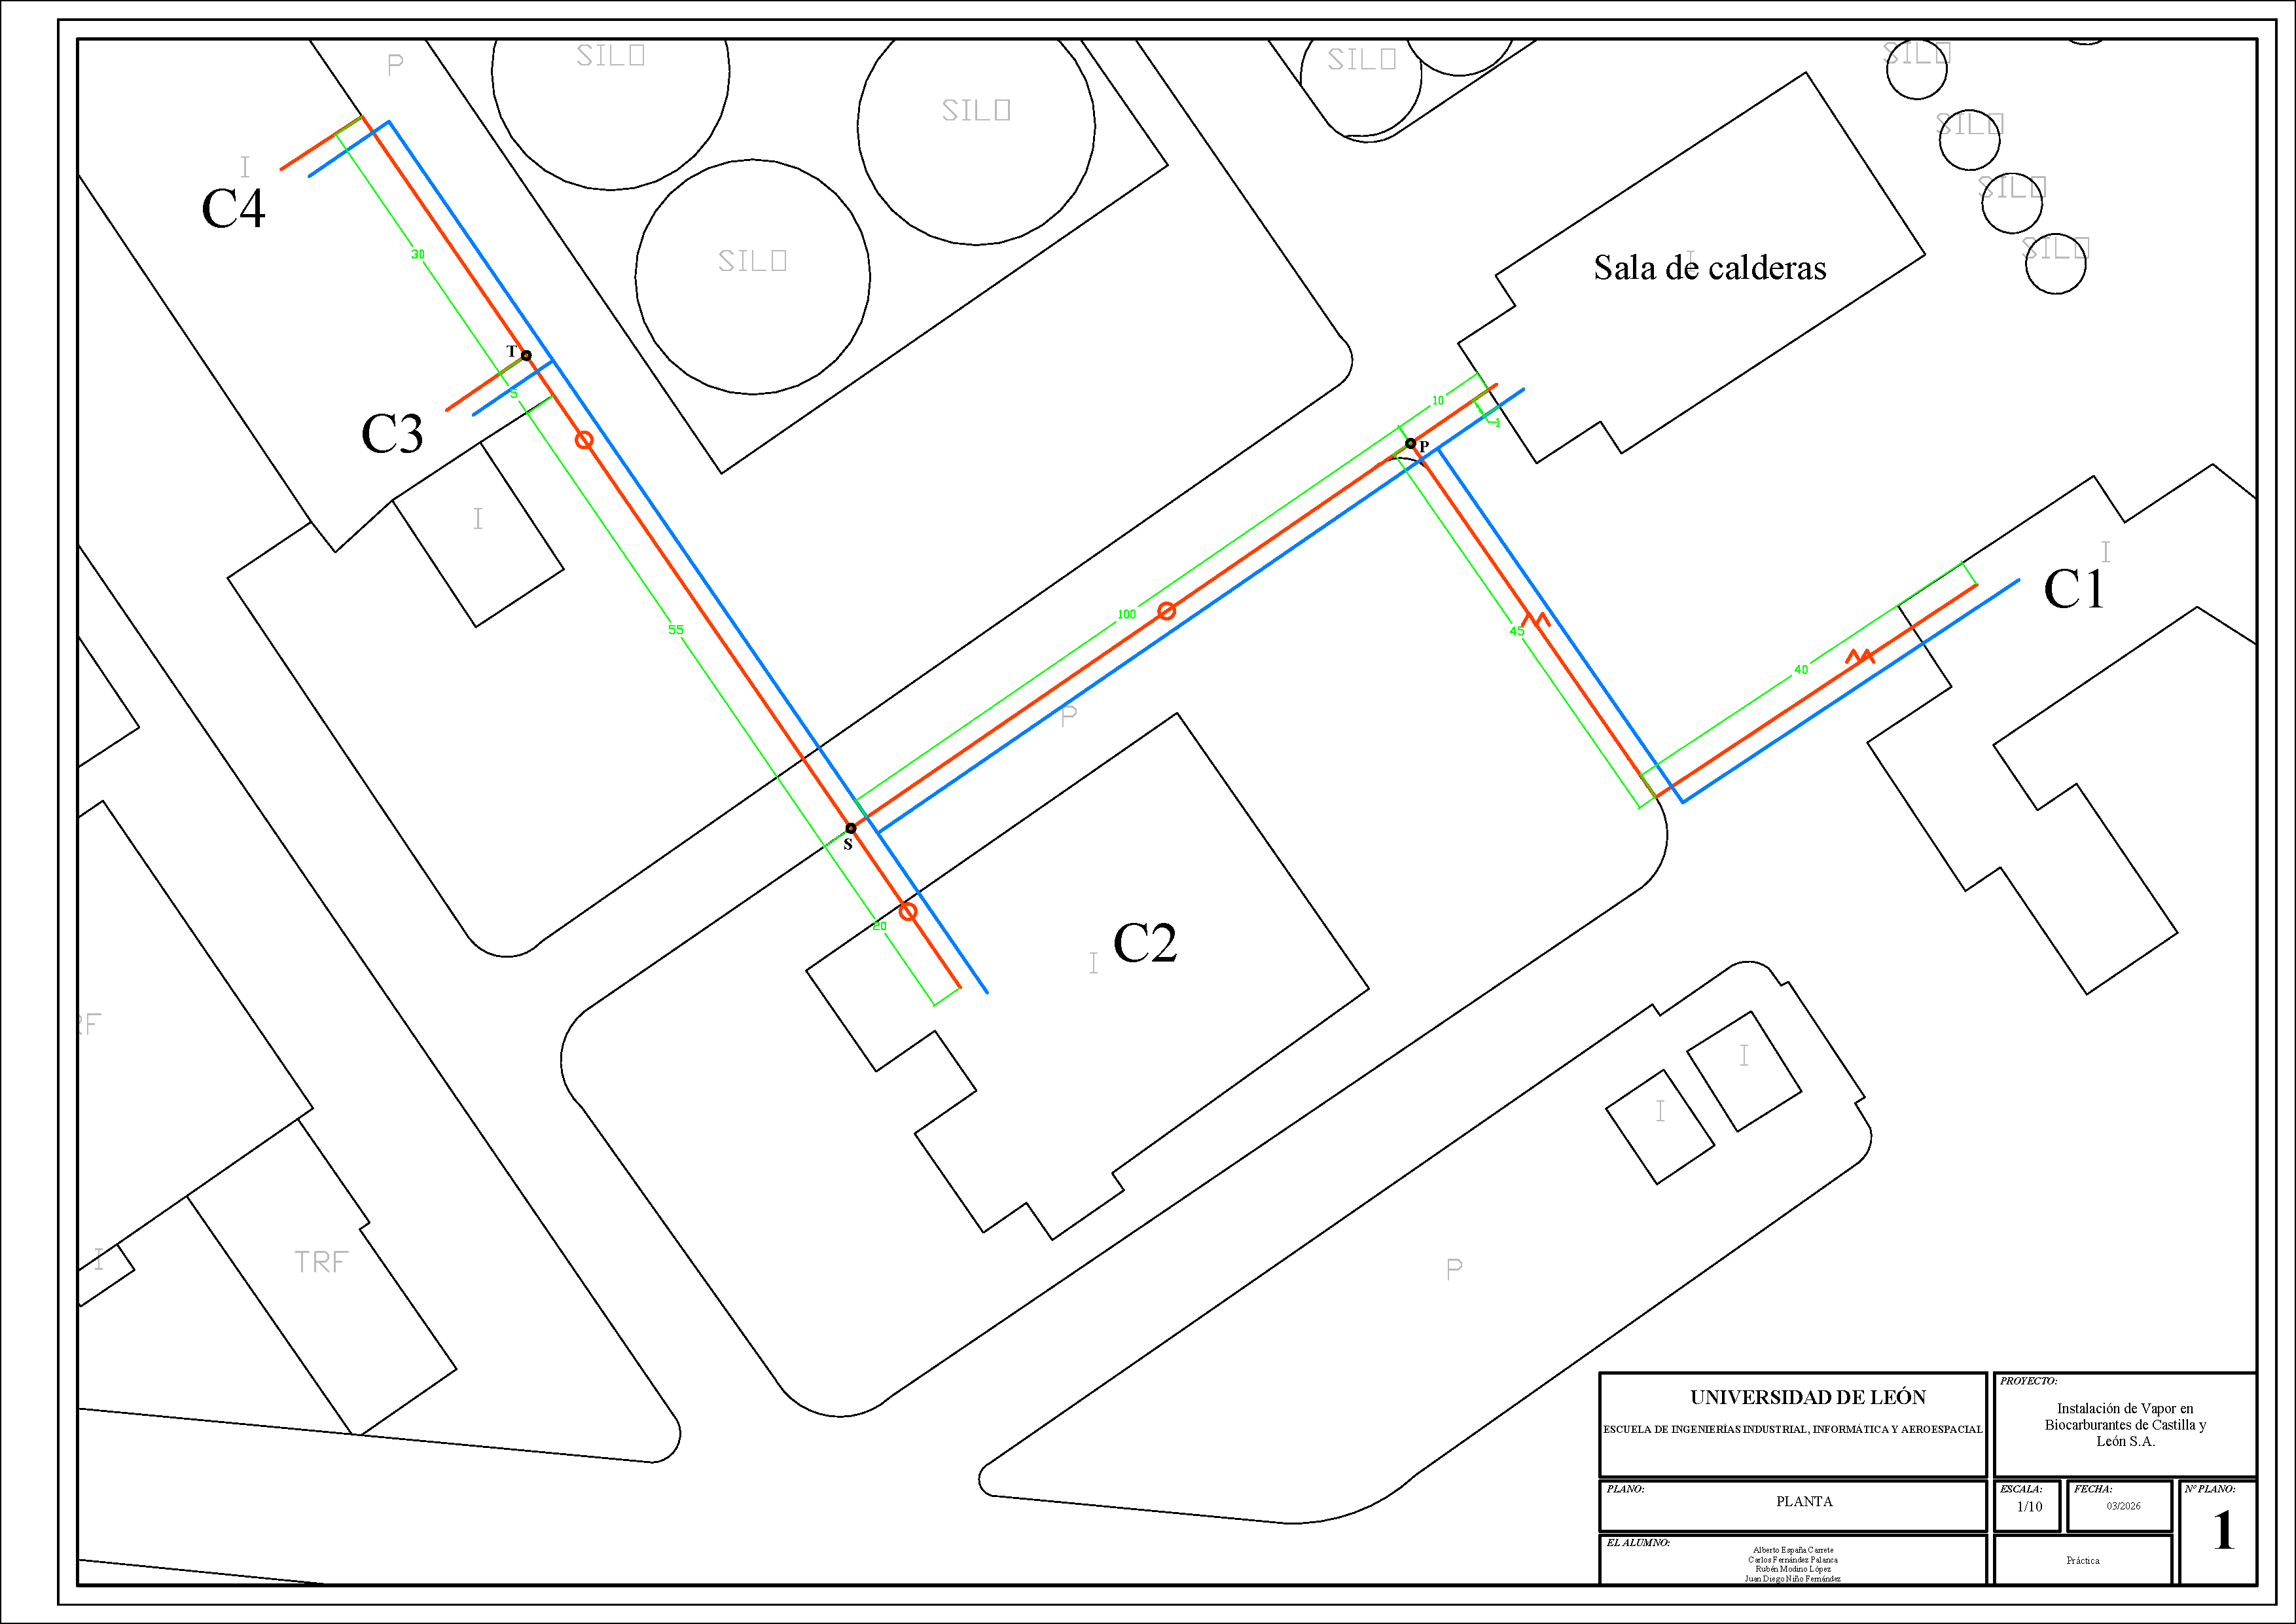
\includepdf[
	pages=-,
	pagecommand={\thispagestyle{empty}},
	fitpaper=true
]{Figuras/planos/plano_vapor-Instalacion.pdf}

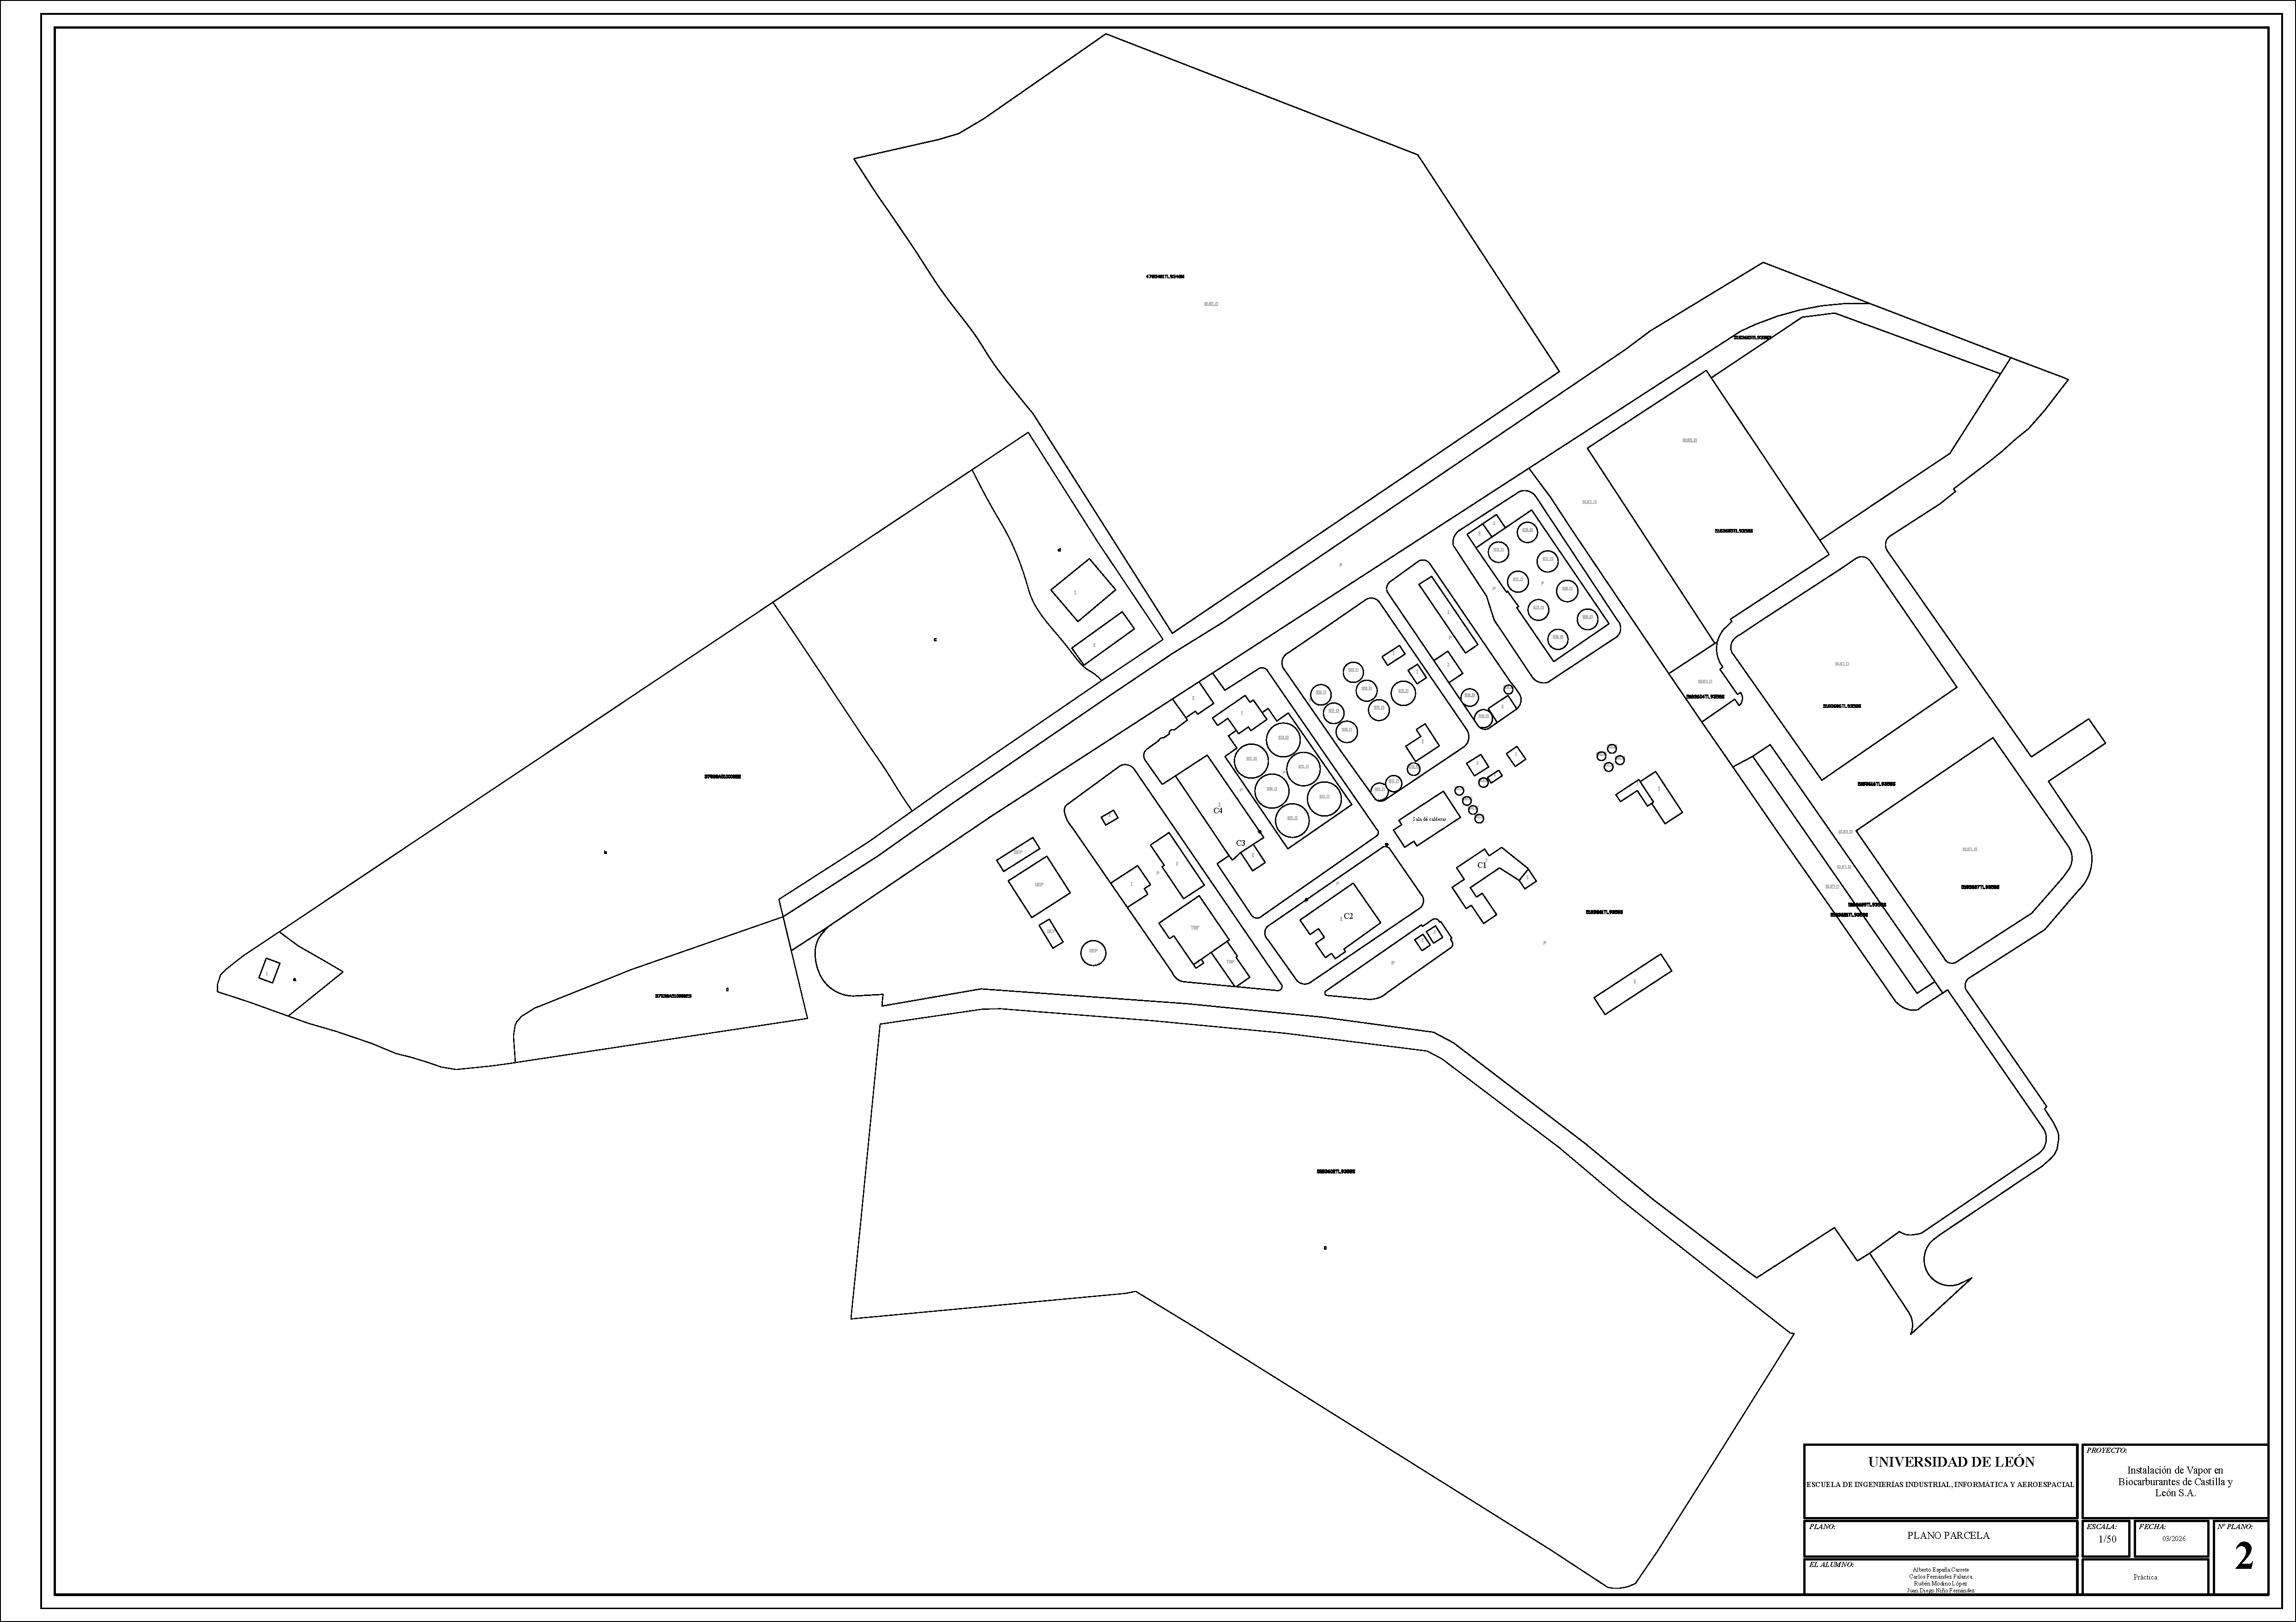
\includepdf[
	pages=-,
	pagecommand={\thispagestyle{empty}},
	fitpaper=true
]{Figuras/planos/plano_vapor-Parcela.pdf}

\myappendix{Diagramas esquemáticos de tramos}
\label{anexo:diagramas}

Este anejo recopila los diagramas esquemáticos de todos los tramos de la red de distribución de vapor y la red de retorno de condensados.

\subsection*{Red de Vapor}

\begin{figure}[H]
	\centering
	
\includegraphics[trim = {2cm  6cm 2cm 5cm }, clip=true, width=0.6\textwidth]{Figuras/dibujos_tramos/Vapor_TR1_Caldera-P.pdf}
	\caption{Esquema del Tramo 1 de Vapor (Caldera-P). Fuente: Elaboración grupal.}
	\label{fig:anejo2-vapor-tr1}
\end{figure}

\begin{figure}[H]
	\centering
	
\includegraphics[trim = {0.7cm  5cm 1cm 5cm }, clip=true, width=0.6\textwidth]{Figuras/dibujos_tramos/Vapor_TR2_P-C1.pdf}
	\caption{Esquema del Tramo 2 de Vapor (P-C1). Fuente: Elaboración grupal.}
	\label{fig:anejo2-vapor-tr2}
\end{figure}

\begin{figure}[H]
	\centering
	
\includegraphics[trim = {0.5cm  6cm 1.7cm 3cm }, clip=true, width=0.6\textwidth]{Figuras/dibujos_tramos/Vapor_TR3_P-S.pdf}
	\caption{Esquema del Tramo 3 de Vapor (P-S). Fuente: Elaboración grupal.}
	\label{fig:anejo2-vapor-tr3}
\end{figure}

\begin{figure}[H]
	\centering
	
\includegraphics[trim = {2cm  5cm 2cm 3.5cm }, clip=true, width=0.5\textwidth]{Figuras/dibujos_tramos/Vapor_TR4_S-C2.pdf}
	\caption{Esquema del Tramo 4 de Vapor (S-C2). Fuente: Elaboración grupal.}
	\label{fig:anejo2-vapor-tr4}
\end{figure}

\begin{figure}[H]
	\centering
	
\includegraphics[trim = {1cm  5cm 1cm 4.5cm }, clip=true, width=0.6\textwidth]{Figuras/dibujos_tramos/Vapor_TR5_S-T.pdf}
	\caption{Esquema del Tramo 5 de Vapor (S-T). Fuente: Elaboración grupal.}
	\label{fig:anejo2-vapor-tr5}
\end{figure}

\begin{figure}[H]
	\centering
	
\includegraphics[trim = {2cm  6cm 2cm 5cm }, clip=true, width=0.5\textwidth]{Figuras/dibujos_tramos/Vapor_TR6_T-C3.pdf}
	\caption{Esquema del Tramo 6 de Vapor (T-C3). Fuente: Elaboración grupal.}
	\label{fig:anejo2-vapor-tr6}
\end{figure}

\begin{figure}[H]
	\centering
	
\includegraphics[trim = {1cm  10cm 1cm 1cm }, clip=true, width=0.6\textwidth]{Figuras/dibujos_tramos/Vapor_TR7_T-C4.pdf}
	\caption{Esquema del Tramo 7 de Vapor (T-C4). Fuente: Elaboración grupal.}
	\label{fig:anejo2-vapor-tr7}
\end{figure}

\subsection*{Red de Condensados}

\begin{figure}[H]
	\centering
	
\includegraphics[trim = {1cm  6cm 0.5cm 3cm }, clip=true, width=0.6\textwidth]{Figuras/dibujos_tramos/Condensados_TR1_Caldera-P.pdf}
	\caption{Esquema del Tramo 1 de Condensados (Caldera-P). Fuente: Elaboración grupal.}
	\label{fig:anejo2-condensados-tr1}
\end{figure}

\begin{figure}[H]
	\centering
	
\includegraphics[trim = {1cm  8cm 2cm 4cm }, clip=true, width=0.7\textwidth]{Figuras/dibujos_tramos/Condensados_TR2_P-C1.pdf}
	\caption{Esquema del Tramo 2 de Condensados (P-C1). Fuente: Elaboración grupal.}
	\label{fig:anejo2-condensados-tr2}
\end{figure}

\begin{figure}[H]
	\centering
	
\includegraphics[trim = {1cm  6cm 2cm 4cm }, clip=true, width=0.6\textwidth]{Figuras/dibujos_tramos/Condensados_TR3_P-S.pdf}
	\caption{Esquema del Tramo 3 de Condensados (P-S). Fuente: Elaboración grupal.}
	\label{fig:anejo2-condensados-tr3}
\end{figure}

\begin{figure}[H]
	\centering
	
\includegraphics[trim = {2cm  6cm 2cm 3.5cm }, clip=true, width=0.5\textwidth]{Figuras/dibujos_tramos/Condensados_TR4_S-C2.pdf}
	\caption{Esquema del Tramo 4 de Condensados (S-C2). Fuente: Elaboración grupal.}
	\label{fig:anejo2-condensados-tr4}
\end{figure}

\begin{figure}[H]
	\centering
	
\includegraphics[trim = {2cm  6cm 2cm 5cm }, clip=true, width=0.6\textwidth]{Figuras/dibujos_tramos/Condensados_TR5_S-T.pdf}
	\caption{Esquema del Tramo 5 de Condensados (S-T). Fuente: Elaboración grupal.}
	\label{fig:anejo2-condensados-tr5}
\end{figure}

\begin{figure}[H]
	\centering
	
\includegraphics[trim = {2cm  6cm 2cm 5cm }, clip=true, width=0.6\textwidth]{Figuras/dibujos_tramos/Condensados_TR6_T-C3.pdf}
	\caption{Esquema del Tramo 6 de Condensados (T-C3). Fuente: Elaboración grupal.}
	\label{fig:anejo2-condensados-tr6}
\end{figure}

\begin{figure}[H]
	\centering
	
\includegraphics[trim = {1cm  11cm 1cm 1cm }, clip=true, width=0.7\textwidth]{Figuras/dibujos_tramos/Condensados_TR7_T-C4.pdf}
	\caption{Esquema del Tramo 7 de Condensados (T-C4). Fuente: Elaboración grupal.}
	\label{fig:anejo2-condensados-tr7}
\end{figure}


\myappendix{Hojas de cálculo de dimensionado hidráulico}
\label{anexo:calculos}

Este anejo recopila las hojas de cálculo detalladas del dimensionado hidráulico de todos los tramos de la red de distribución de vapor y la red de retorno de condensados.

\subsection*{Red de Vapor}

\begin{figure}[H]
	\centering
	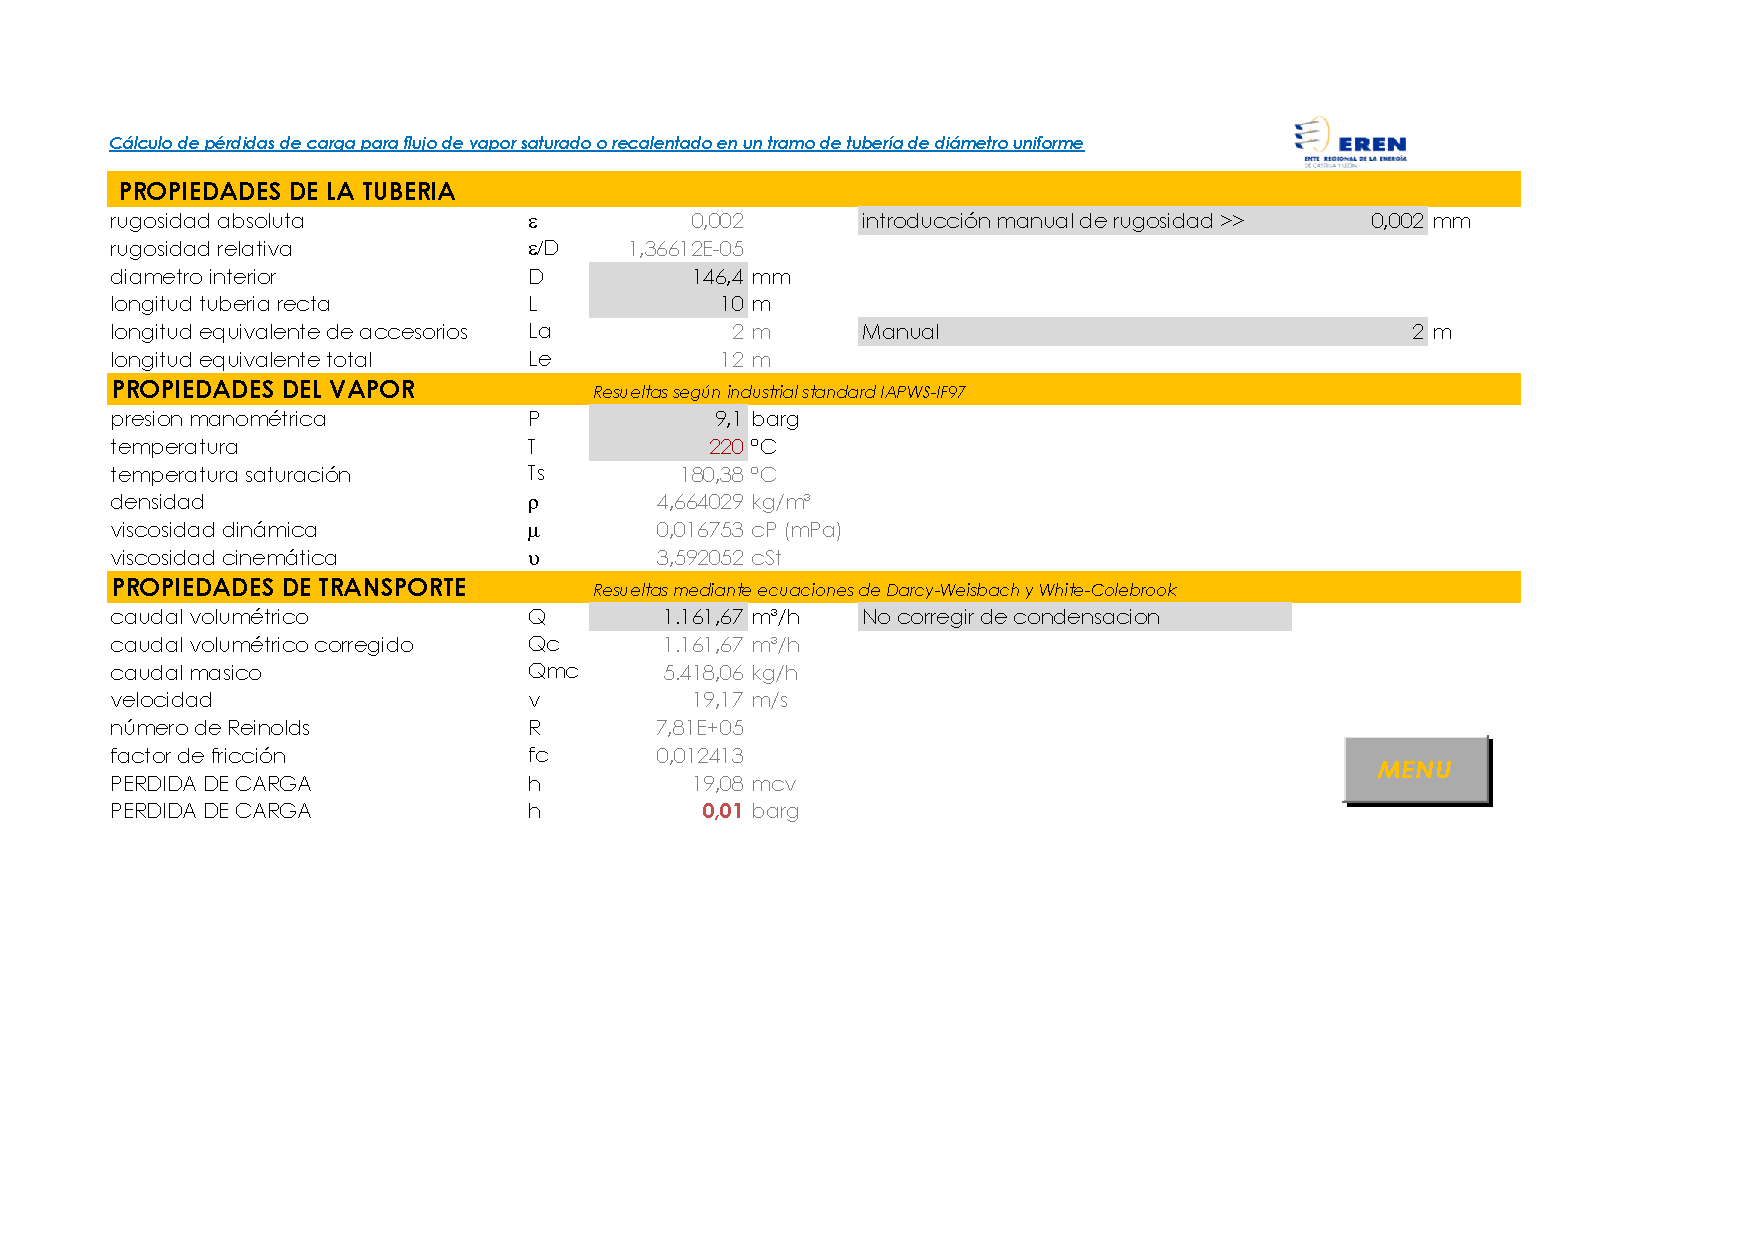
\includegraphics[trim={1cm 5cm 3cm 2cm}, clip = true,width=\textwidth]{Figuras/calculos_tramos/Vapor_TR1_Caldera-P.pdf}
	\caption{Hoja de cálculo del Tramo 1 de Vapor (Caldera-P). Fuente: Elaboración grupal.}
	\label{fig:anejo3-vapor-tr1}
\end{figure}

\begin{figure}[H]
	\centering
	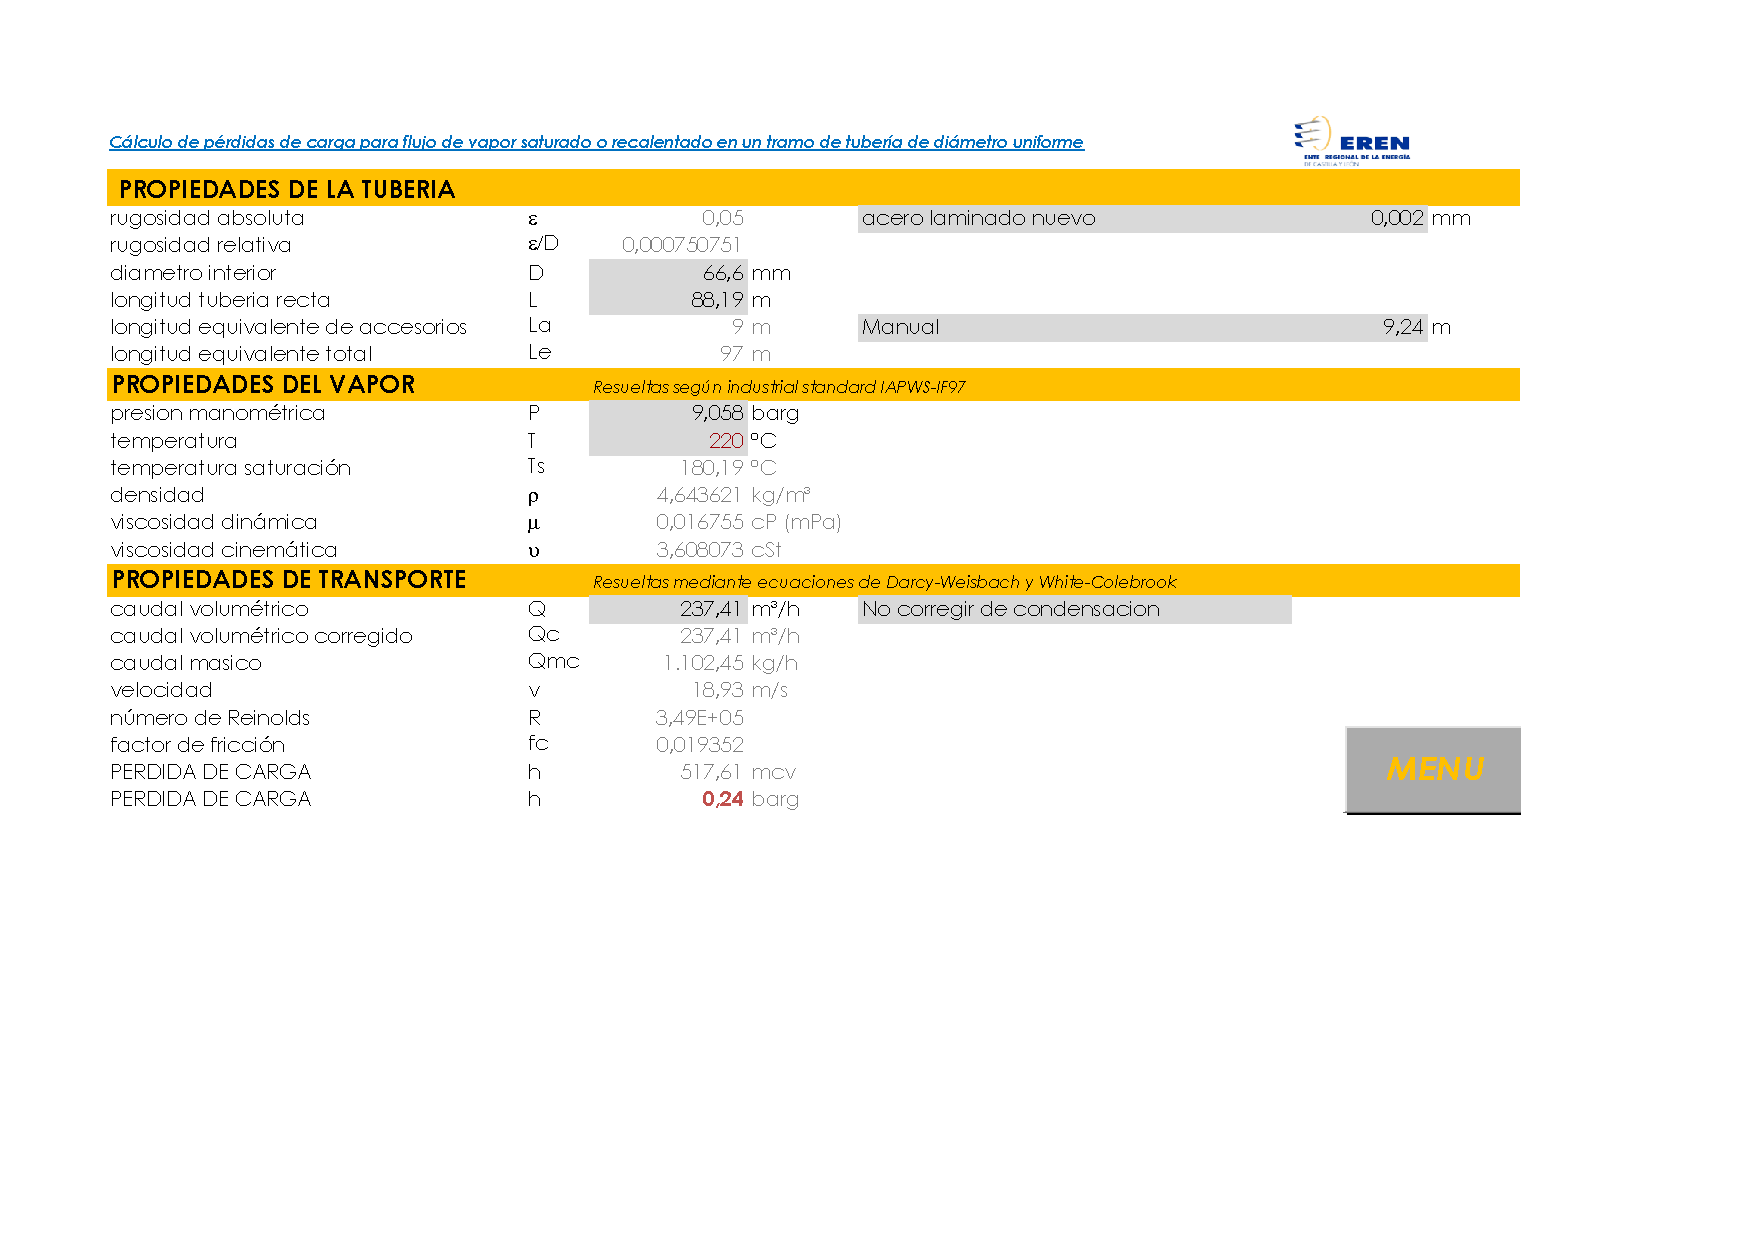
\includegraphics[trim={1cm 5cm 3cm 2cm}, clip = true,width=\textwidth]{Figuras/calculos_tramos/Vapor_TR2_P-C1.pdf}
	\caption{Hoja de cálculo del Tramo 2 de Vapor (P-C1). Fuente: Elaboración grupal.}
	\label{fig:anejo3-vapor-tr2}
\end{figure}

\begin{figure}[H]
	\centering
	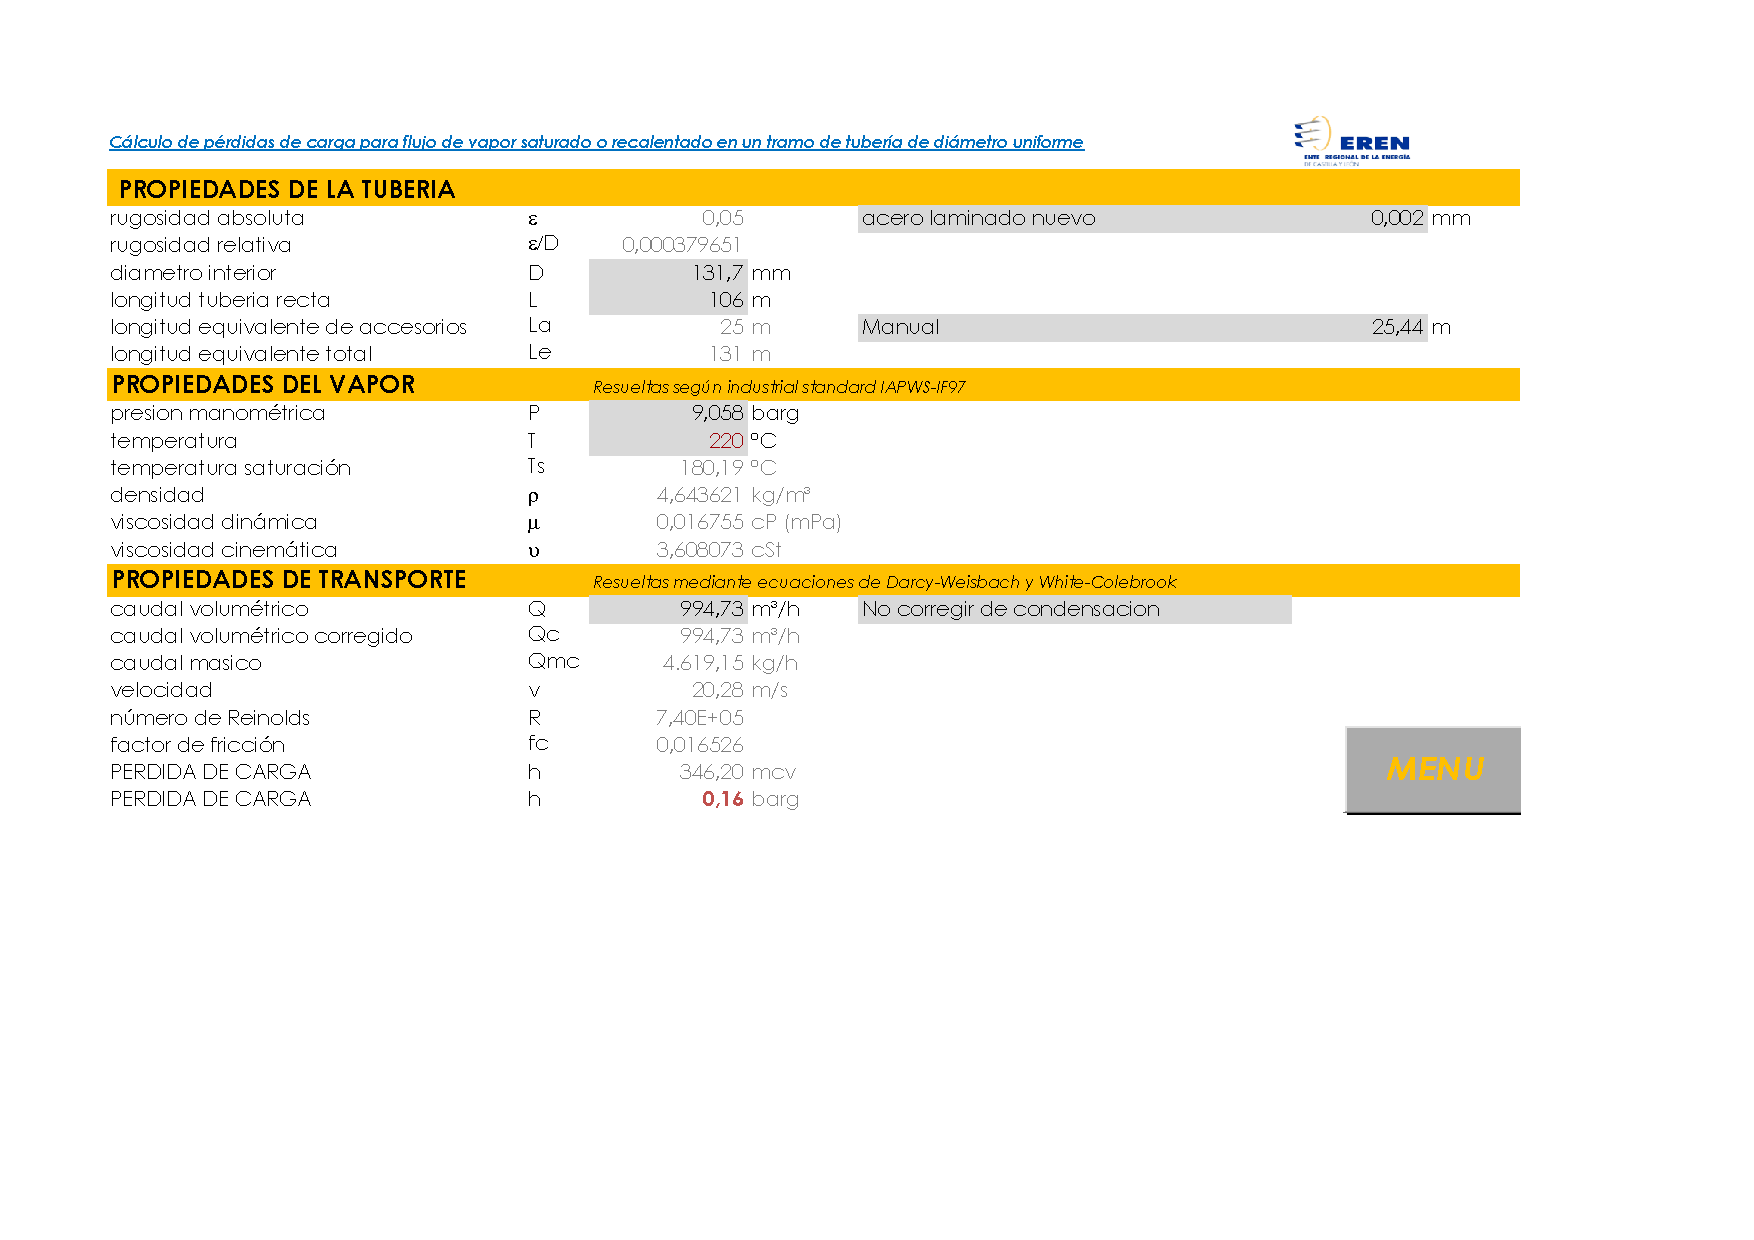
\includegraphics[trim={1cm 5cm 3cm 2cm}, clip = true,width=\textwidth]{Figuras/calculos_tramos/Vapor_TR3_P-S.pdf}
	\caption{Hoja de cálculo del Tramo 3 de Vapor (P-S). Fuente: Elaboración grupal.}
	\label{fig:anejo3-vapor-tr3}
\end{figure}

\begin{figure}[H]
	\centering
	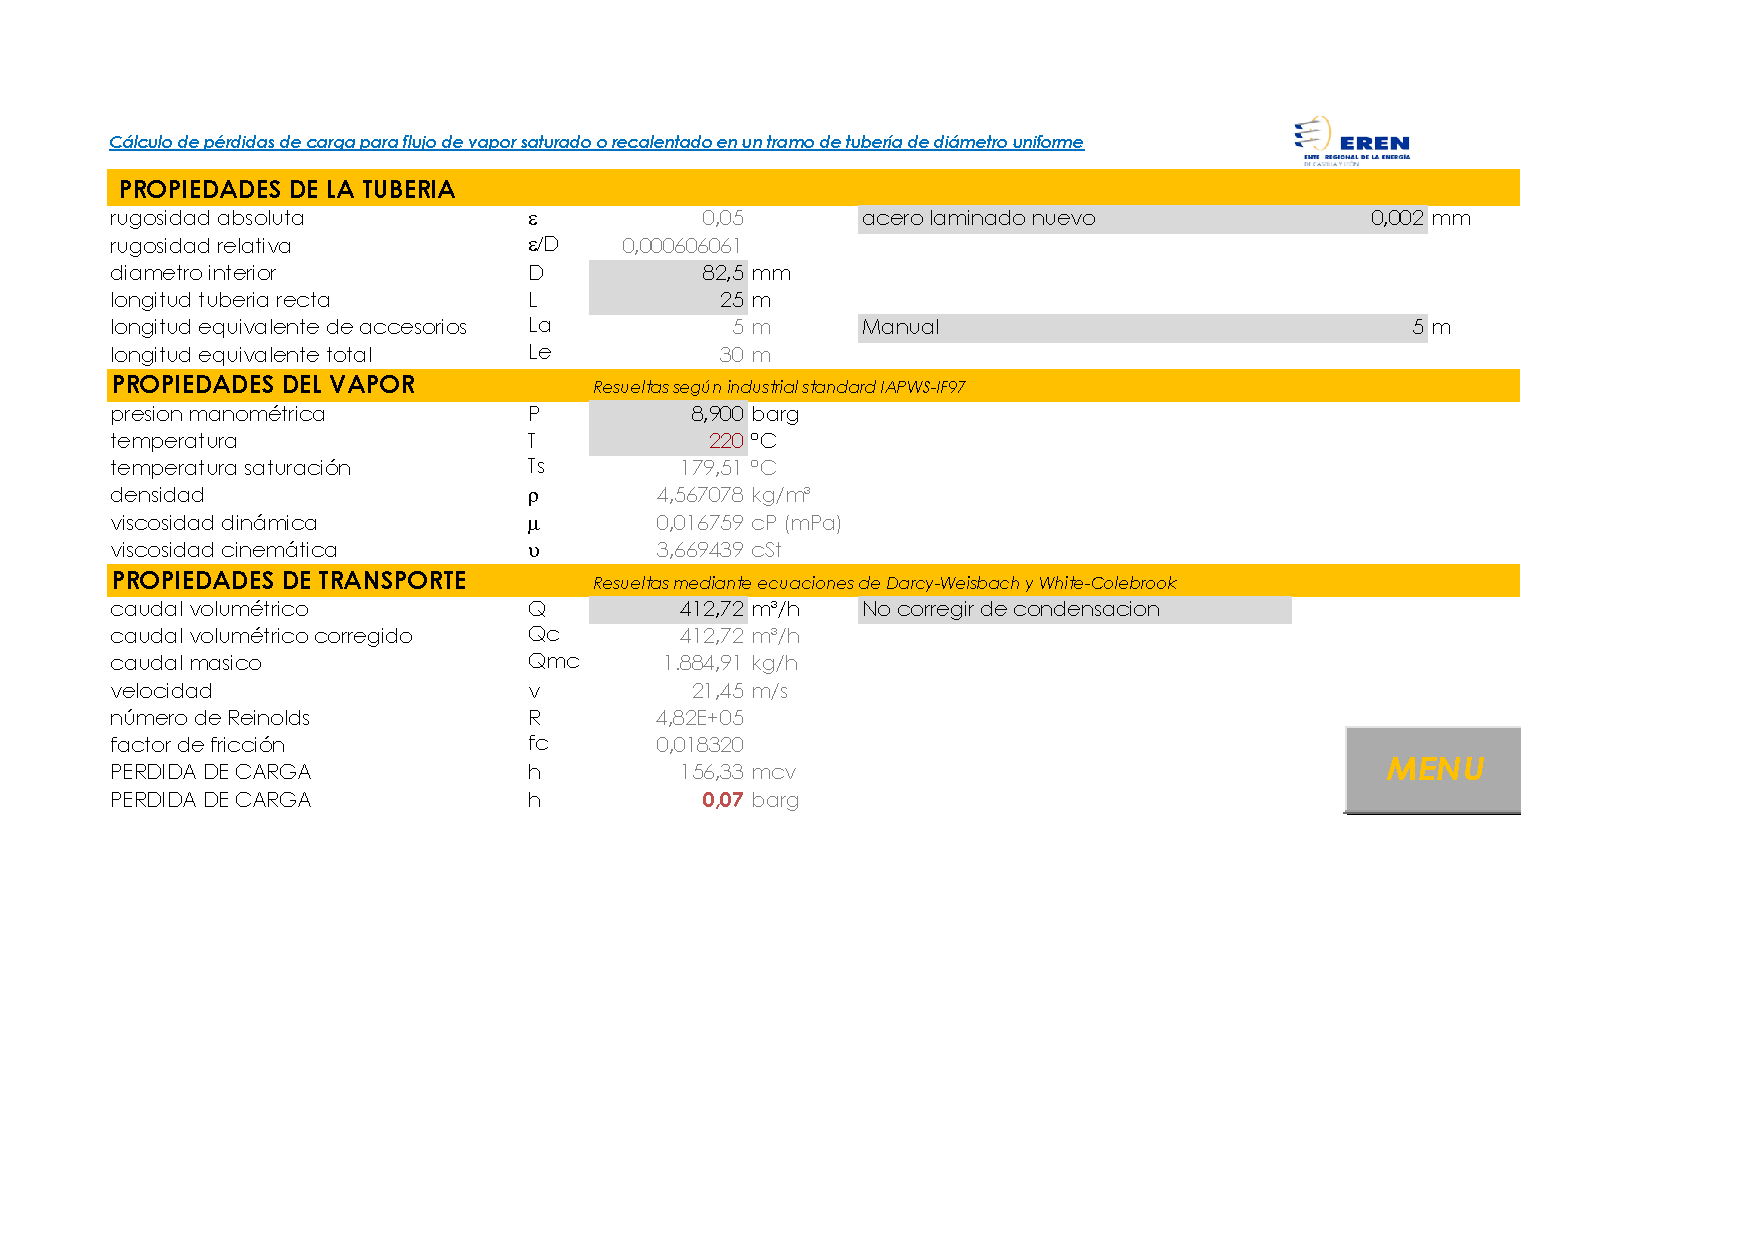
\includegraphics[trim={1cm 5cm 3cm 2cm}, clip = true,width=\textwidth]{Figuras/calculos_tramos/Vapor_TR4_S-C2.pdf}
	\caption{Hoja de cálculo del Tramo 4 de Vapor (S-C2). Fuente: Elaboración grupal.}
	\label{fig:anejo3-vapor-tr4}
\end{figure}

\begin{figure}[H]
	\centering
	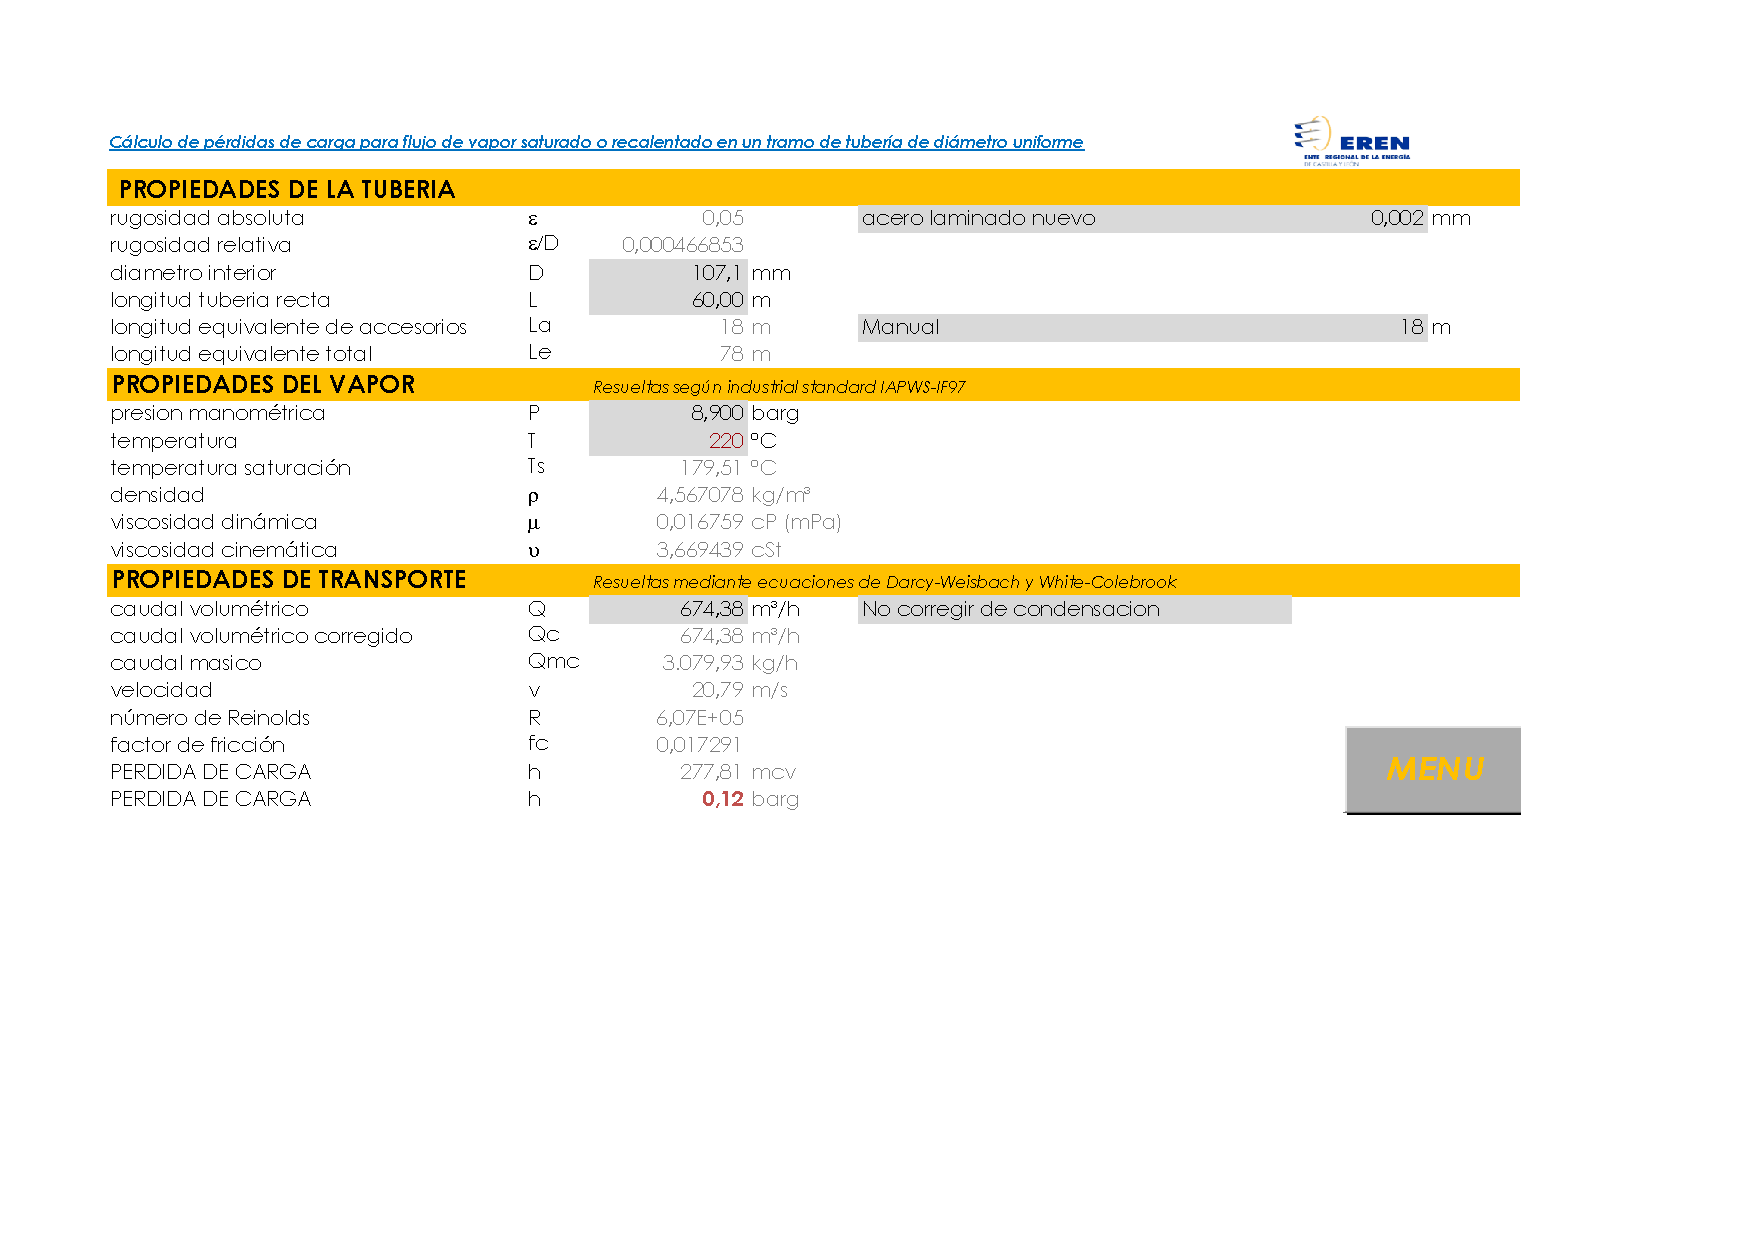
\includegraphics[trim={1cm 5cm 3cm 2cm}, clip = true,width=\textwidth]{Figuras/calculos_tramos/Vapor_TR5_S-T.pdf}
	\caption{Hoja de cálculo del Tramo 5 de Vapor (S-T). Fuente: Elaboración grupal.}
	\label{fig:anejo3-vapor-tr5}
\end{figure}

\begin{figure}[H]
	\centering
	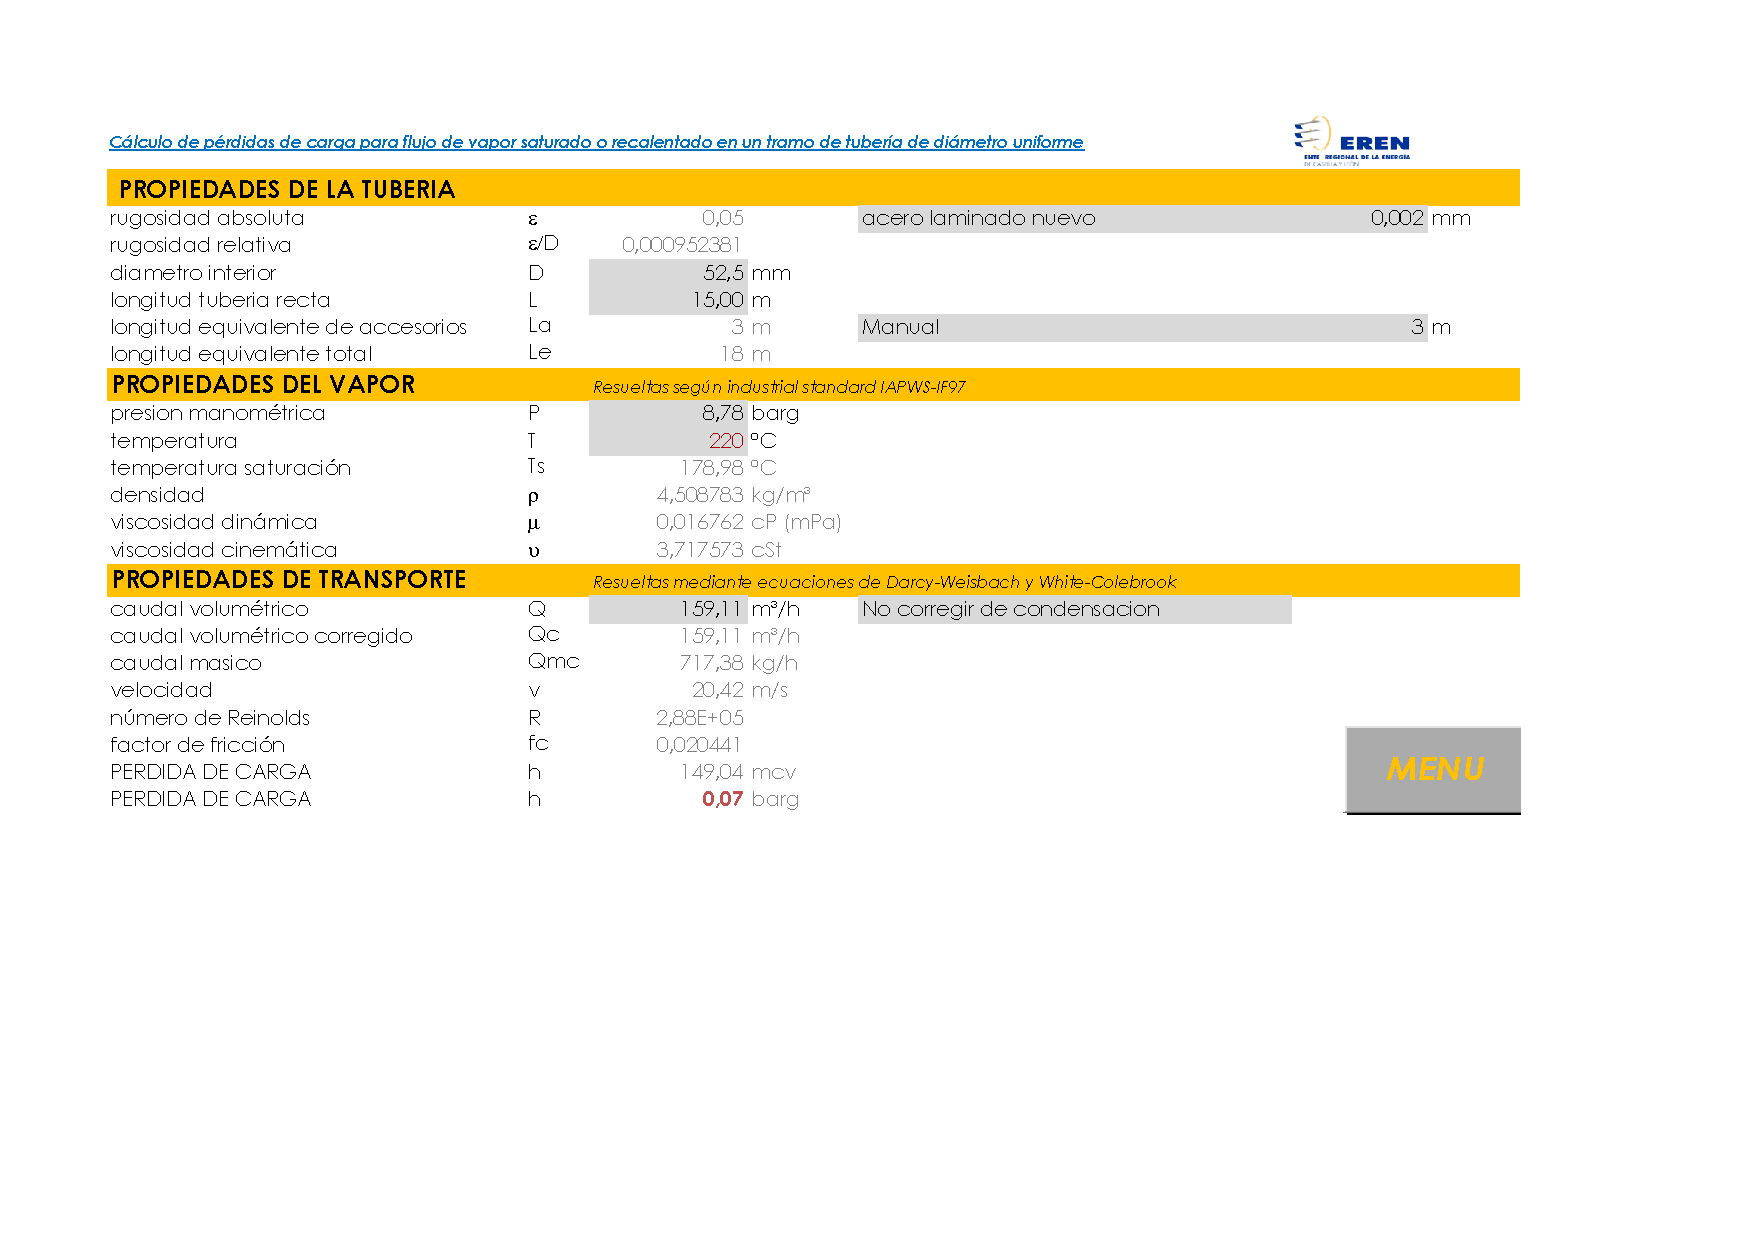
\includegraphics[trim={1cm 5cm 3cm 2cm}, clip = true,width=\textwidth]{Figuras/calculos_tramos/Vapor_TR6_T-C3.pdf}
	\caption{Hoja de cálculo del Tramo 6 de Vapor (T-C3). Fuente: Elaboración grupal.}
	\label{fig:anejo3-vapor-tr6}
\end{figure}

\begin{figure}[H]
	\centering
	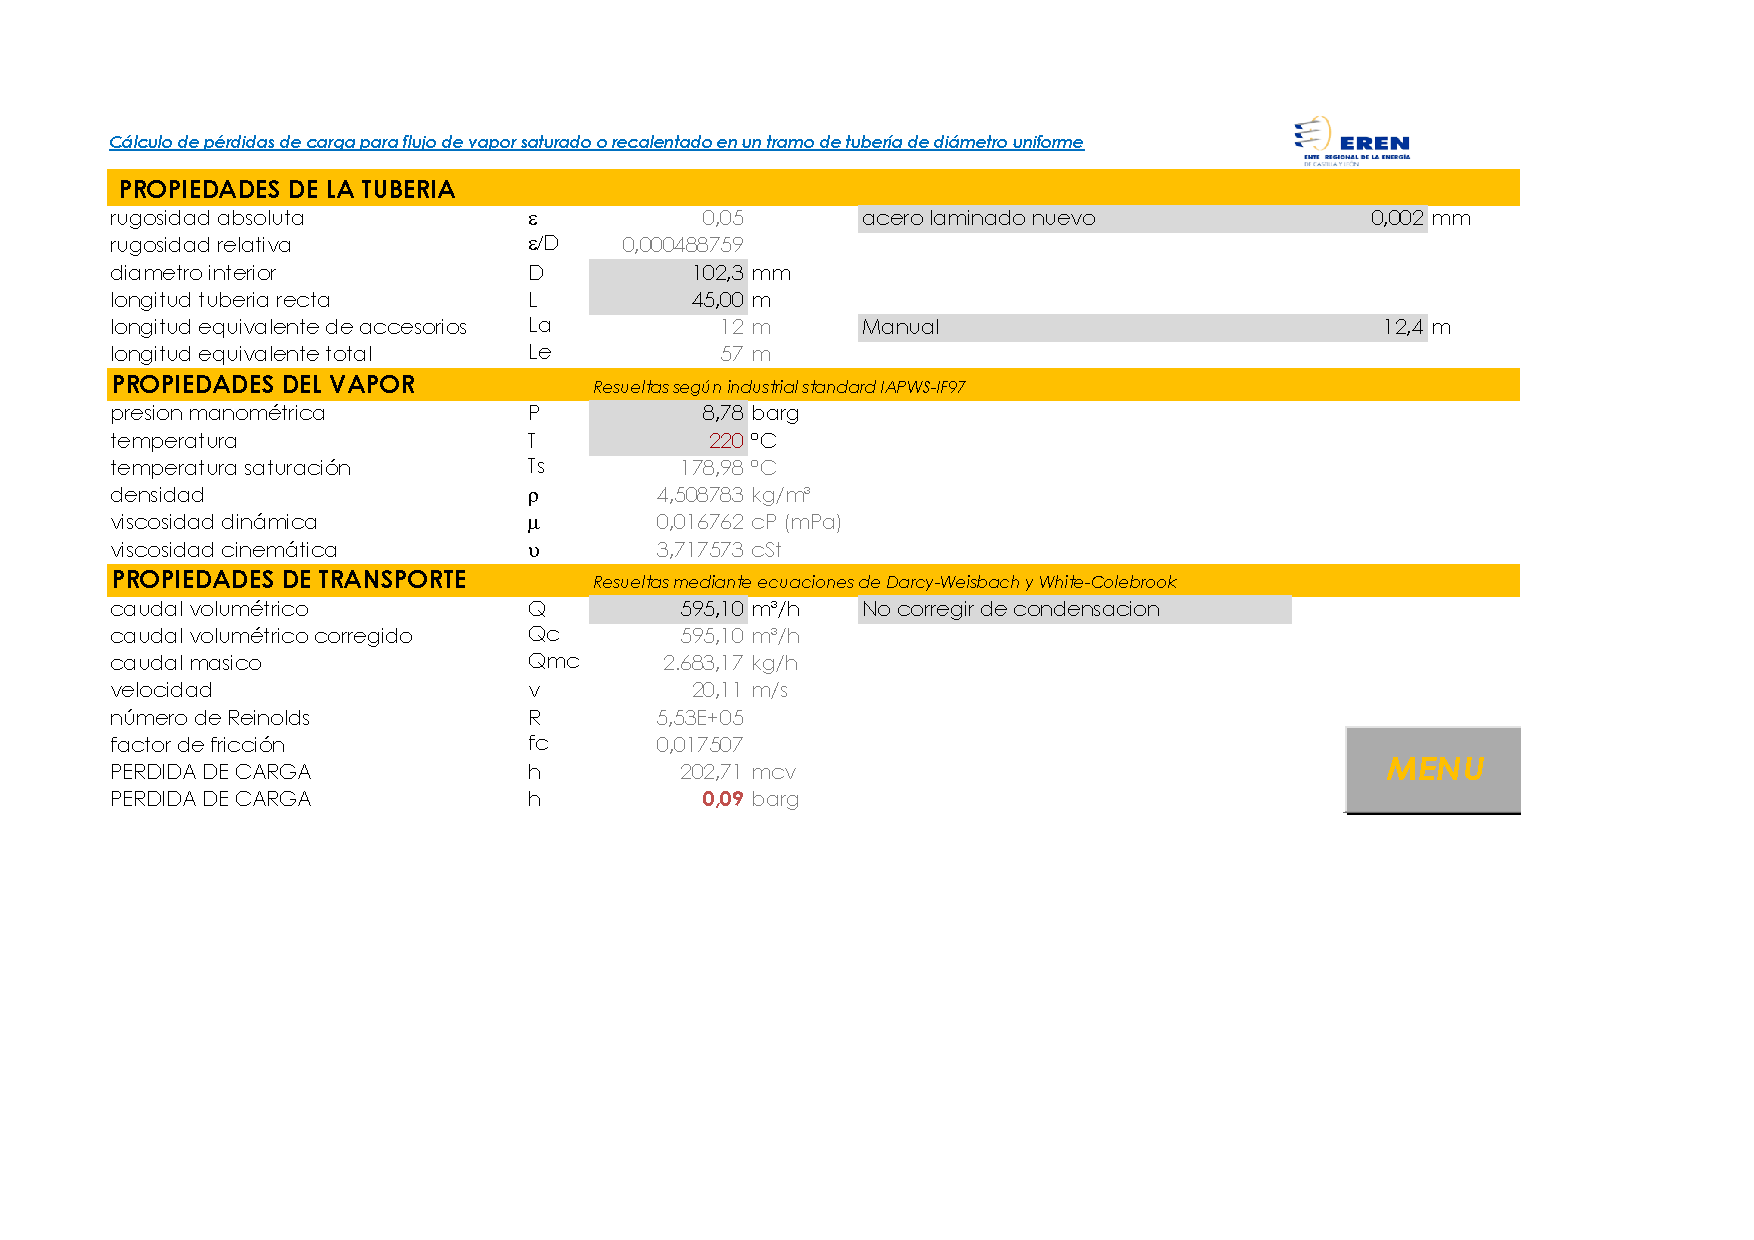
\includegraphics[trim={1cm 5cm 3cm 2cm}, clip = true,width=\textwidth]{Figuras/calculos_tramos/Vapor_TR7_T-C4.pdf}
	\caption{Hoja de cálculo del Tramo 7 de Vapor (T-C4). Fuente: Elaboración grupal.}
	\label{fig:anejo3-vapor-tr7}
\end{figure}

\newpage

\subsection*{Red de Condensados}

\begin{figure}[H]
	\centering
	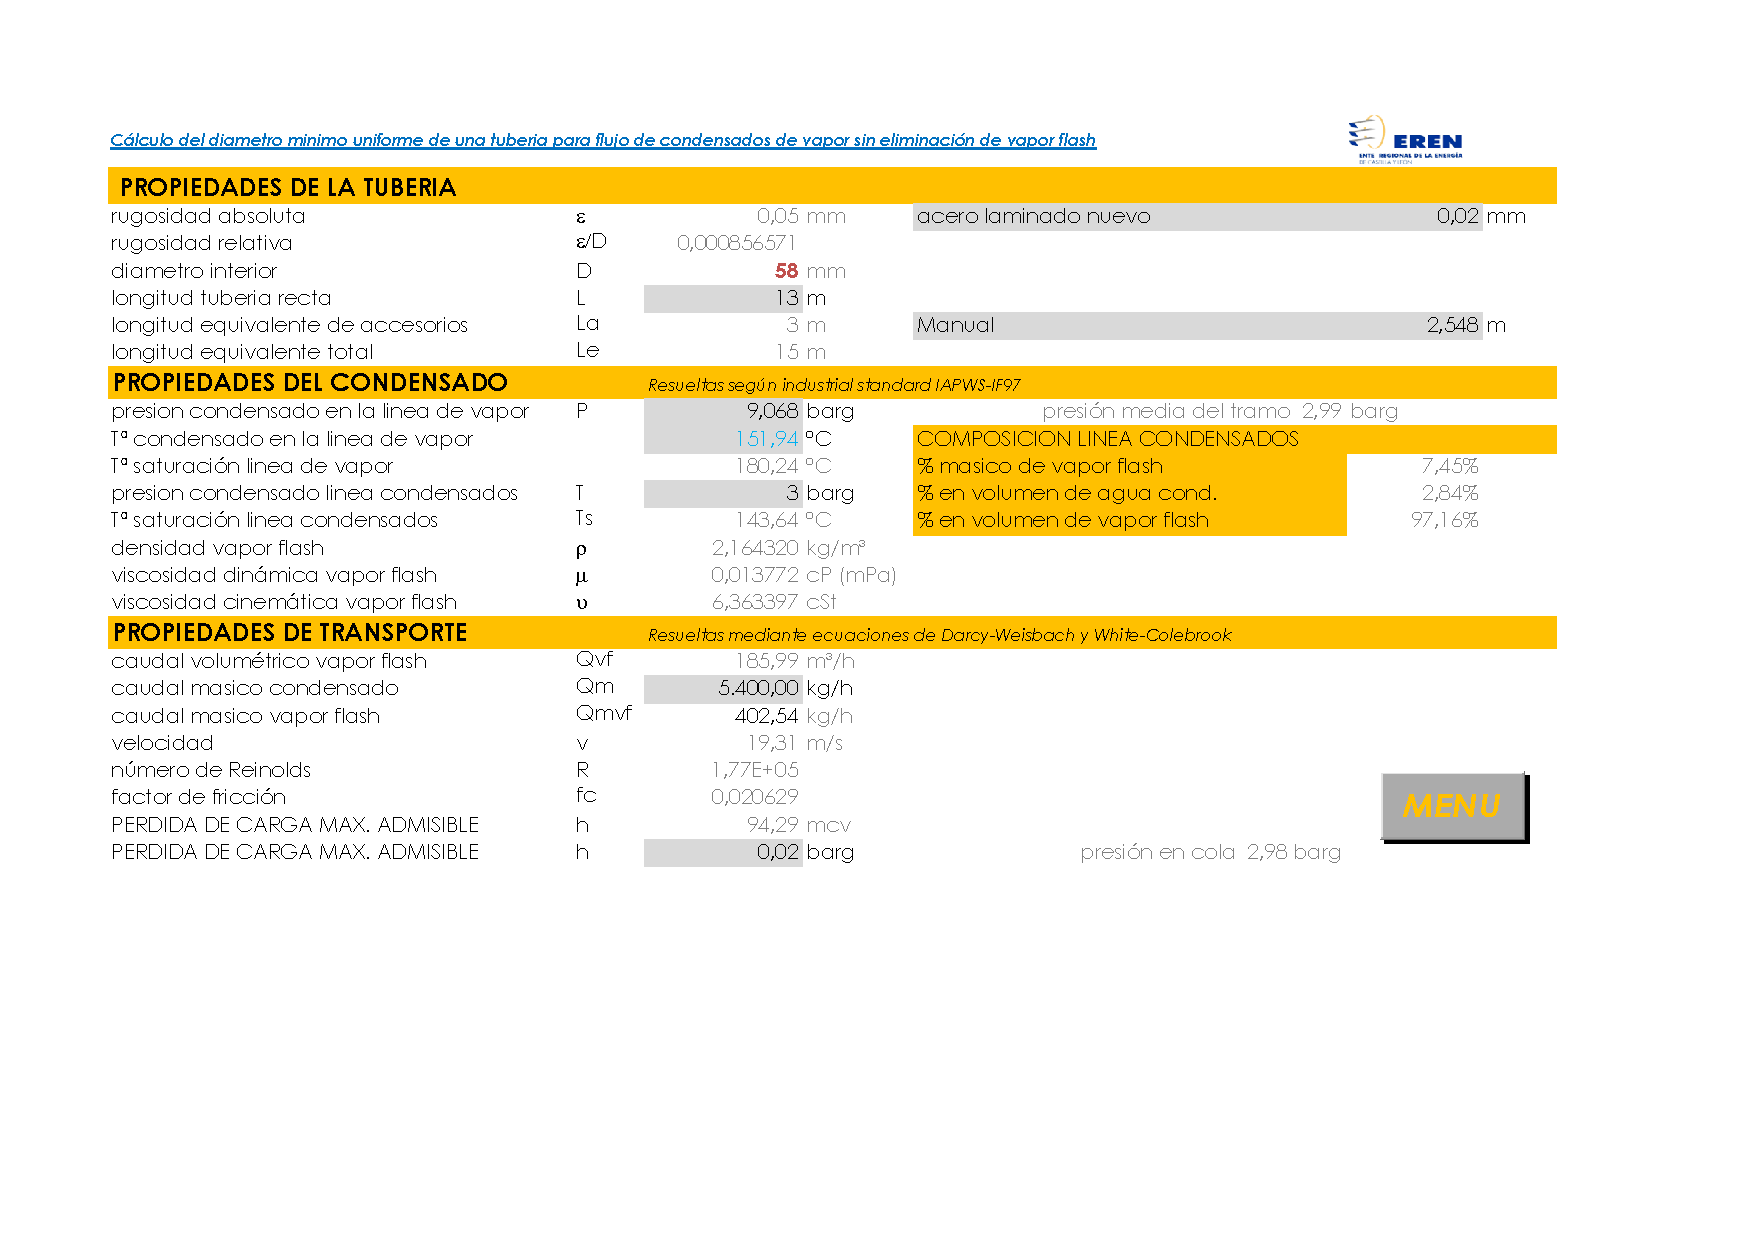
\includegraphics[trim={1cm 5cm 3cm 2cm}, clip = true,width=\textwidth]{Figuras/calculos_tramos/Condensados_TR1_Caldera-P.pdf}
	\caption{Hoja de cálculo del Tramo 1 de Condensados (Caldera-P). Fuente: Elaboración grupal.}
	\label{fig:anejo3-condensados-tr1}
\end{figure}

\begin{figure}[H]
	\centering
	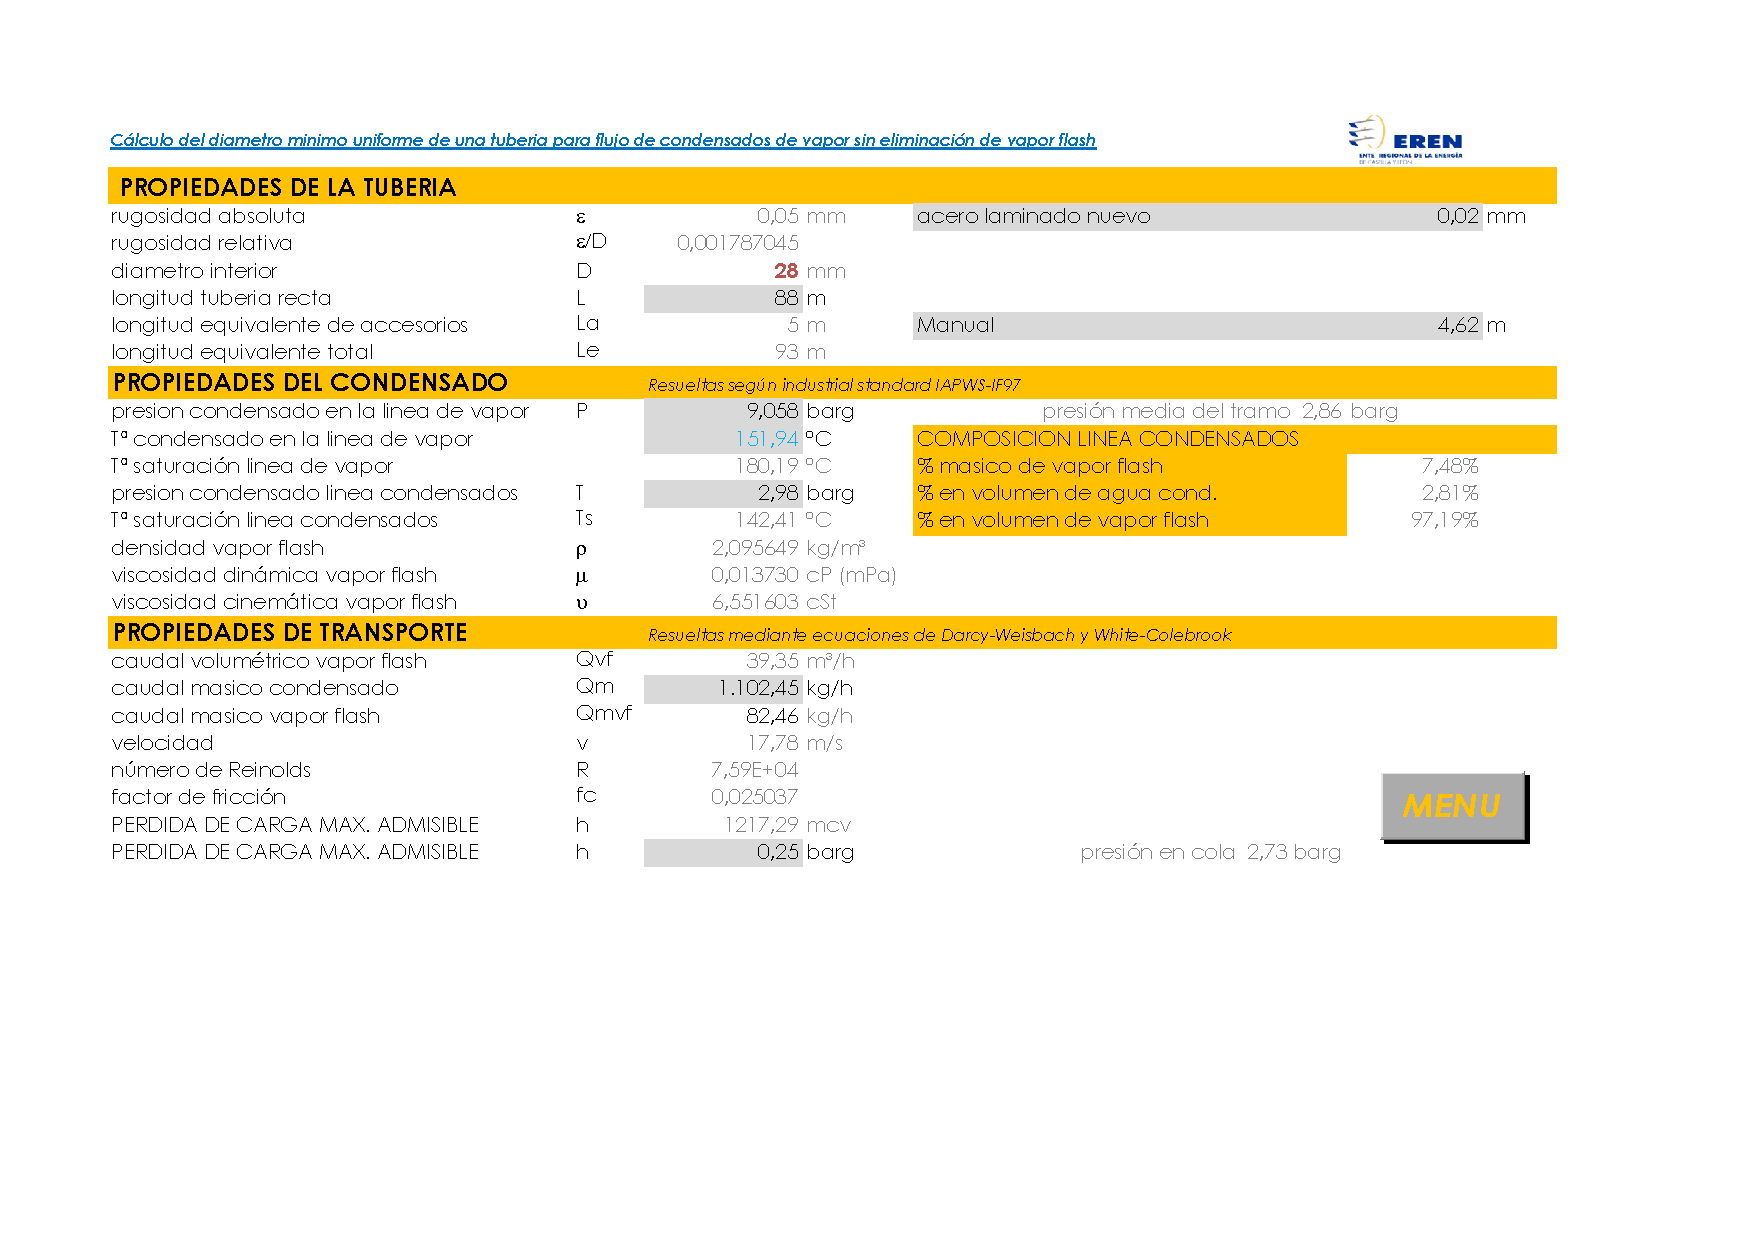
\includegraphics[trim={1cm 5cm 3cm 2cm}, clip = true,width=\textwidth]{Figuras/calculos_tramos/Condensados_TR2_P-C1.pdf}
	\caption{Hoja de cálculo del Tramo 2 de Condensados (P-C1). Fuente: Elaboración grupal.}
	\label{fig:anejo3-condensados-tr2}
\end{figure}

\begin{figure}[H]
	\centering
	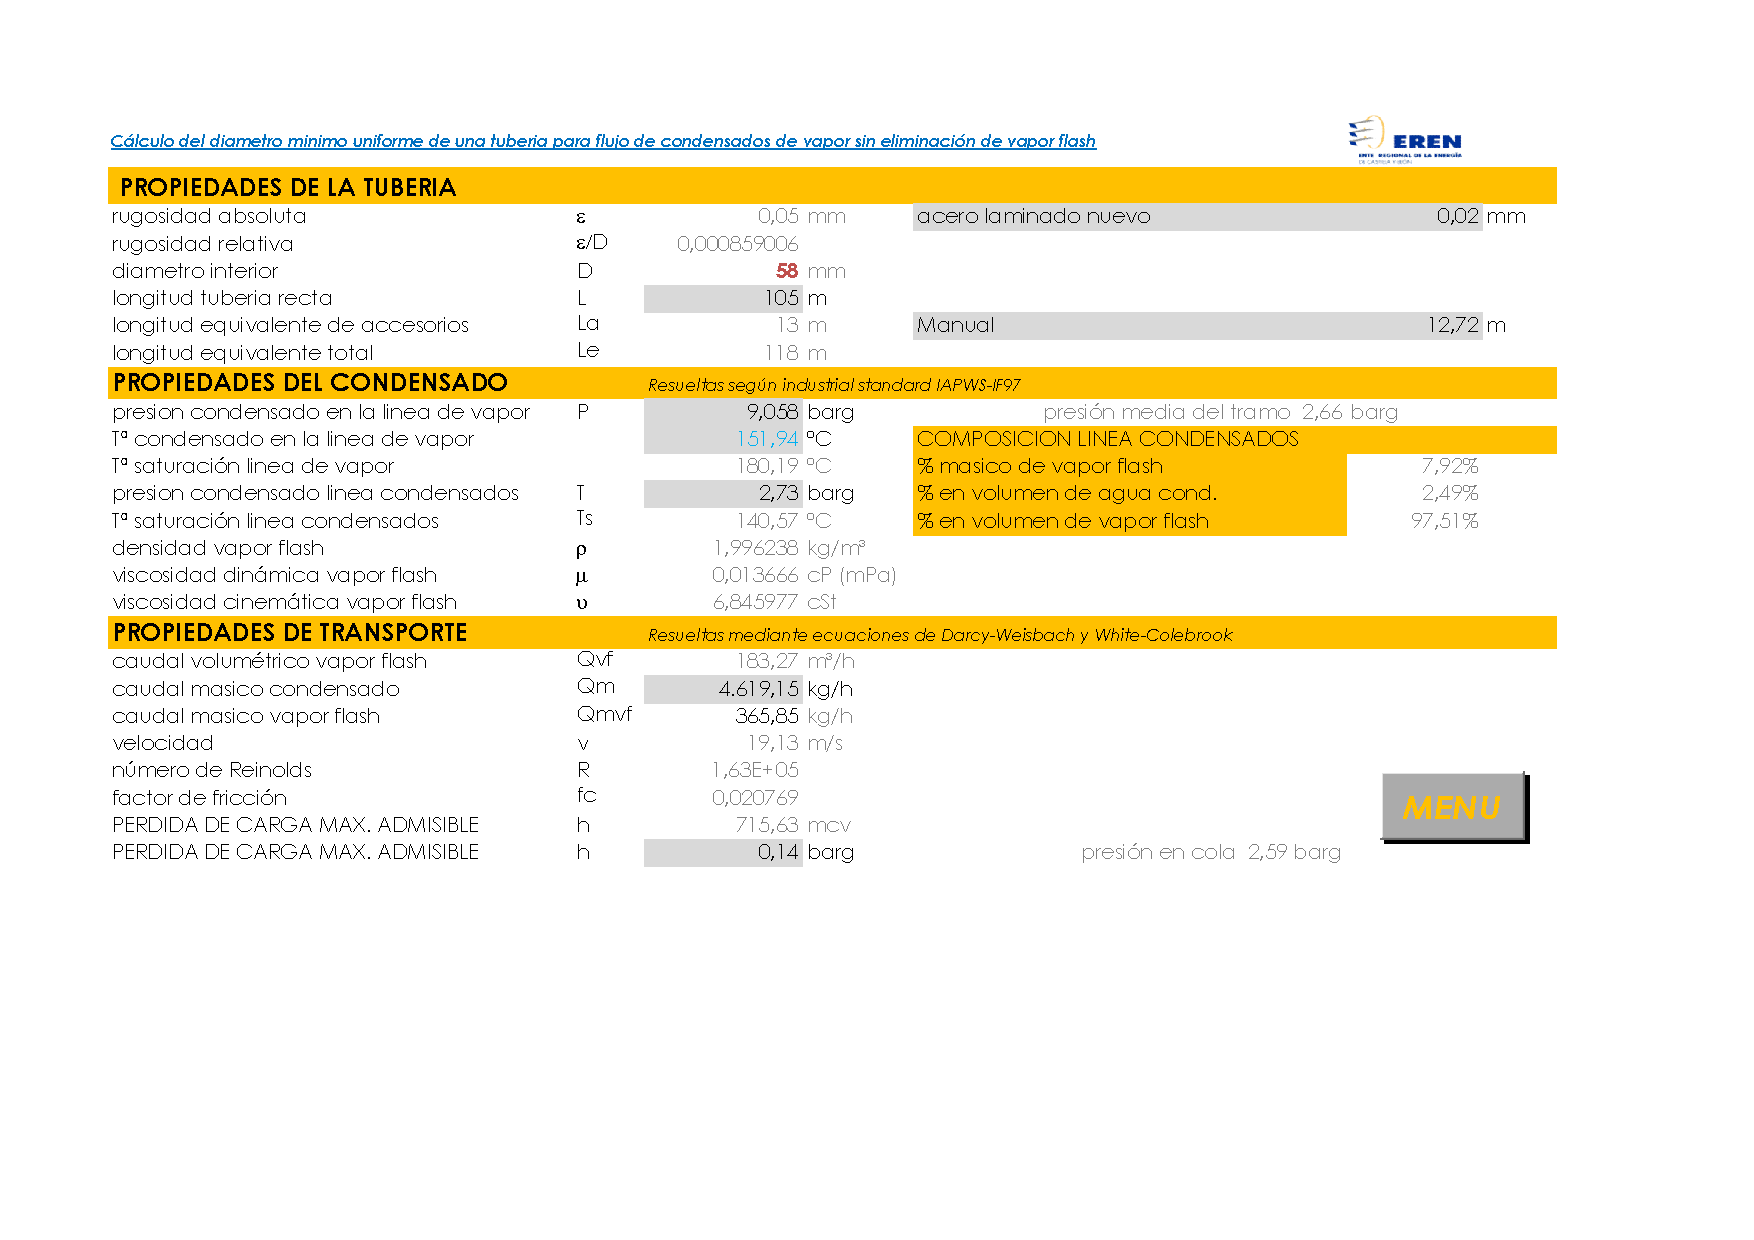
\includegraphics[trim={1cm 5cm 3cm 2cm}, clip = true,width=\textwidth]{Figuras/calculos_tramos/Condensados_TR3_P-S.pdf}
	\caption{Hoja de cálculo del Tramo 3 de Condensados (P-S). Fuente: Elaboración grupal.}
	\label{fig:anejo3-condensados-tr3}
\end{figure}

\begin{figure}[H]
	\centering
	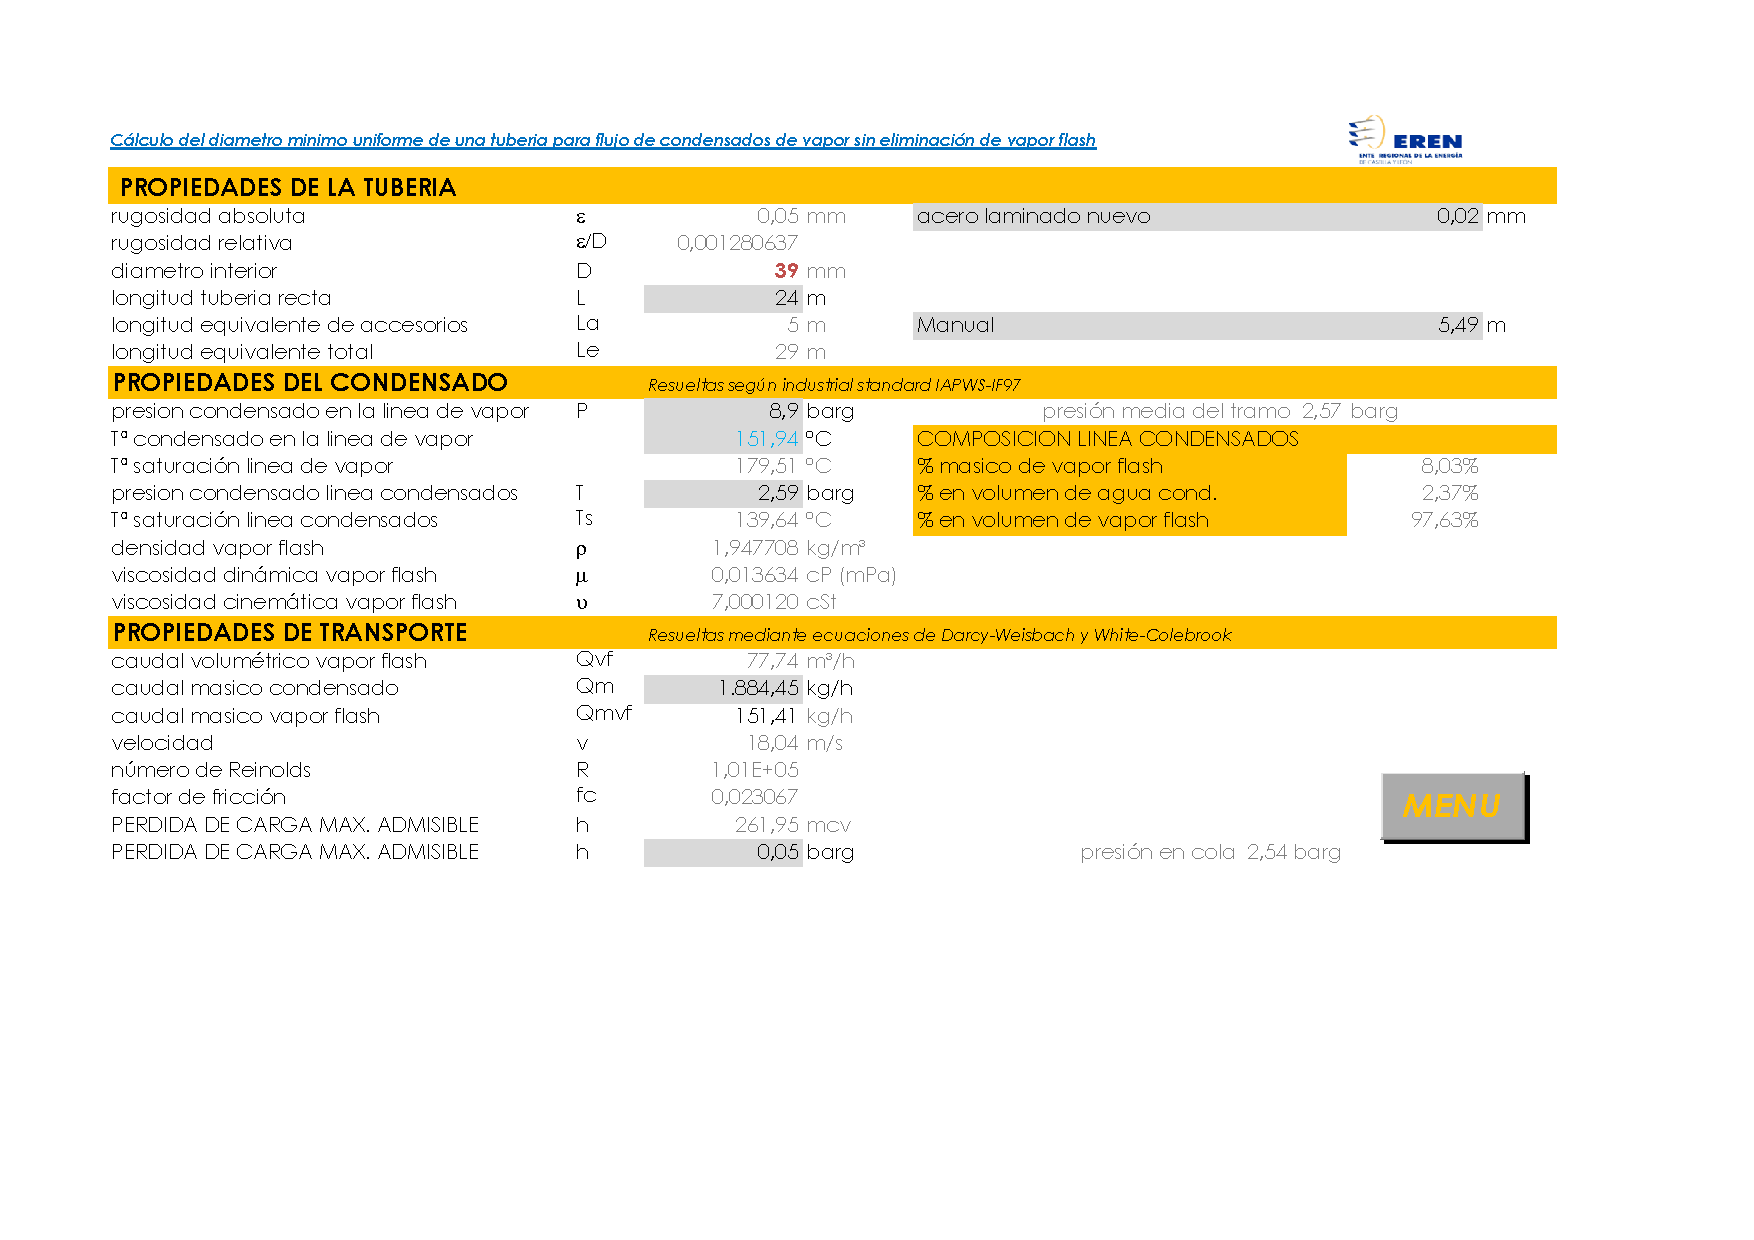
\includegraphics[trim={1cm 5cm 3cm 2cm}, clip = true,width=\textwidth]{Figuras/calculos_tramos/Condensados_TR4_S-C2.pdf}
	\caption{Hoja de cálculo del Tramo 4 de Condensados (S-C2). Fuente: Elaboración grupal.}
	\label{fig:anejo3-condensados-tr4}
\end{figure}

\begin{figure}[H]
	\centering
	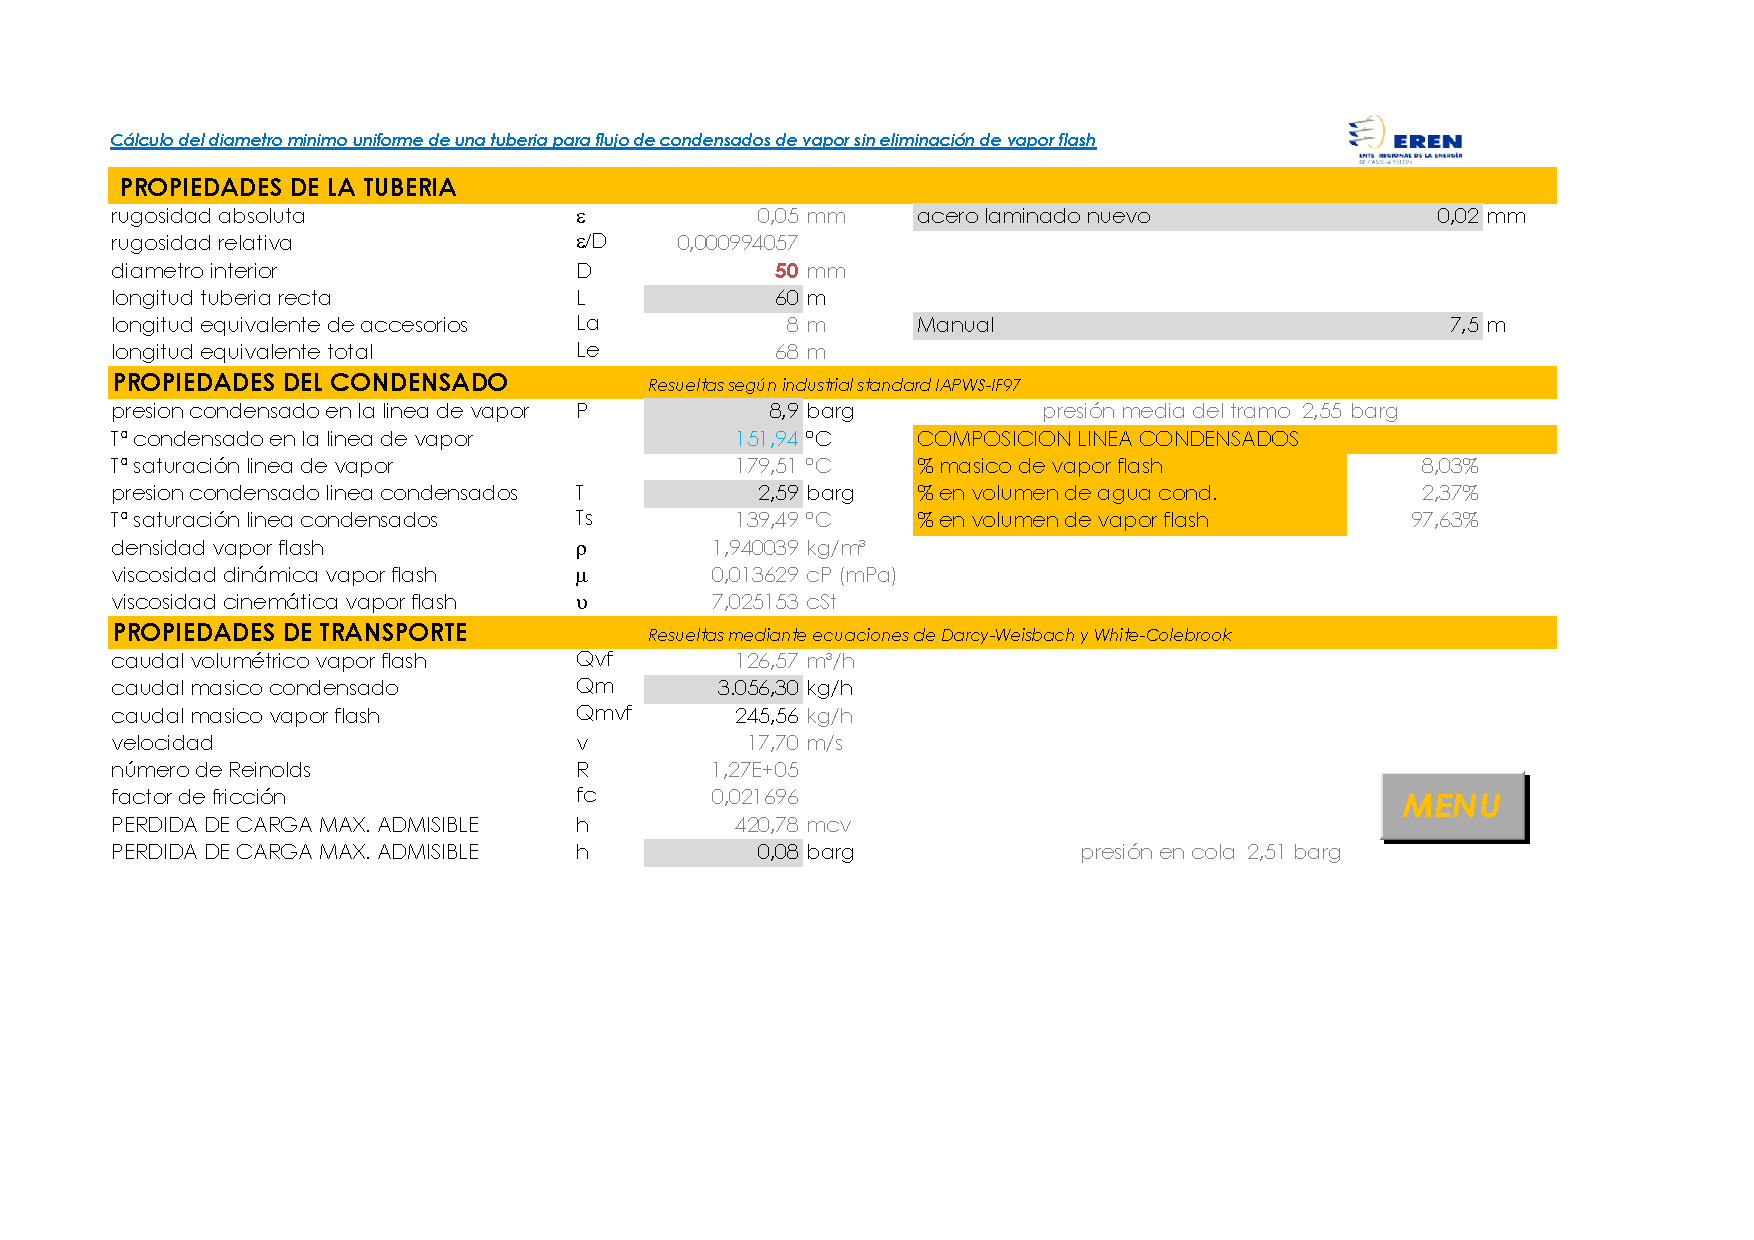
\includegraphics[trim={1cm 5cm 3cm 2cm}, clip = true,width=\textwidth]{Figuras/calculos_tramos/Condensados_TR5_S-T.pdf}
	\caption{Hoja de cálculo del Tramo 5 de Condensados (S-T). Fuente: Elaboración grupal.}
	\label{fig:anejo3-condensados-tr5}
\end{figure}

\begin{figure}[H]
	\centering
	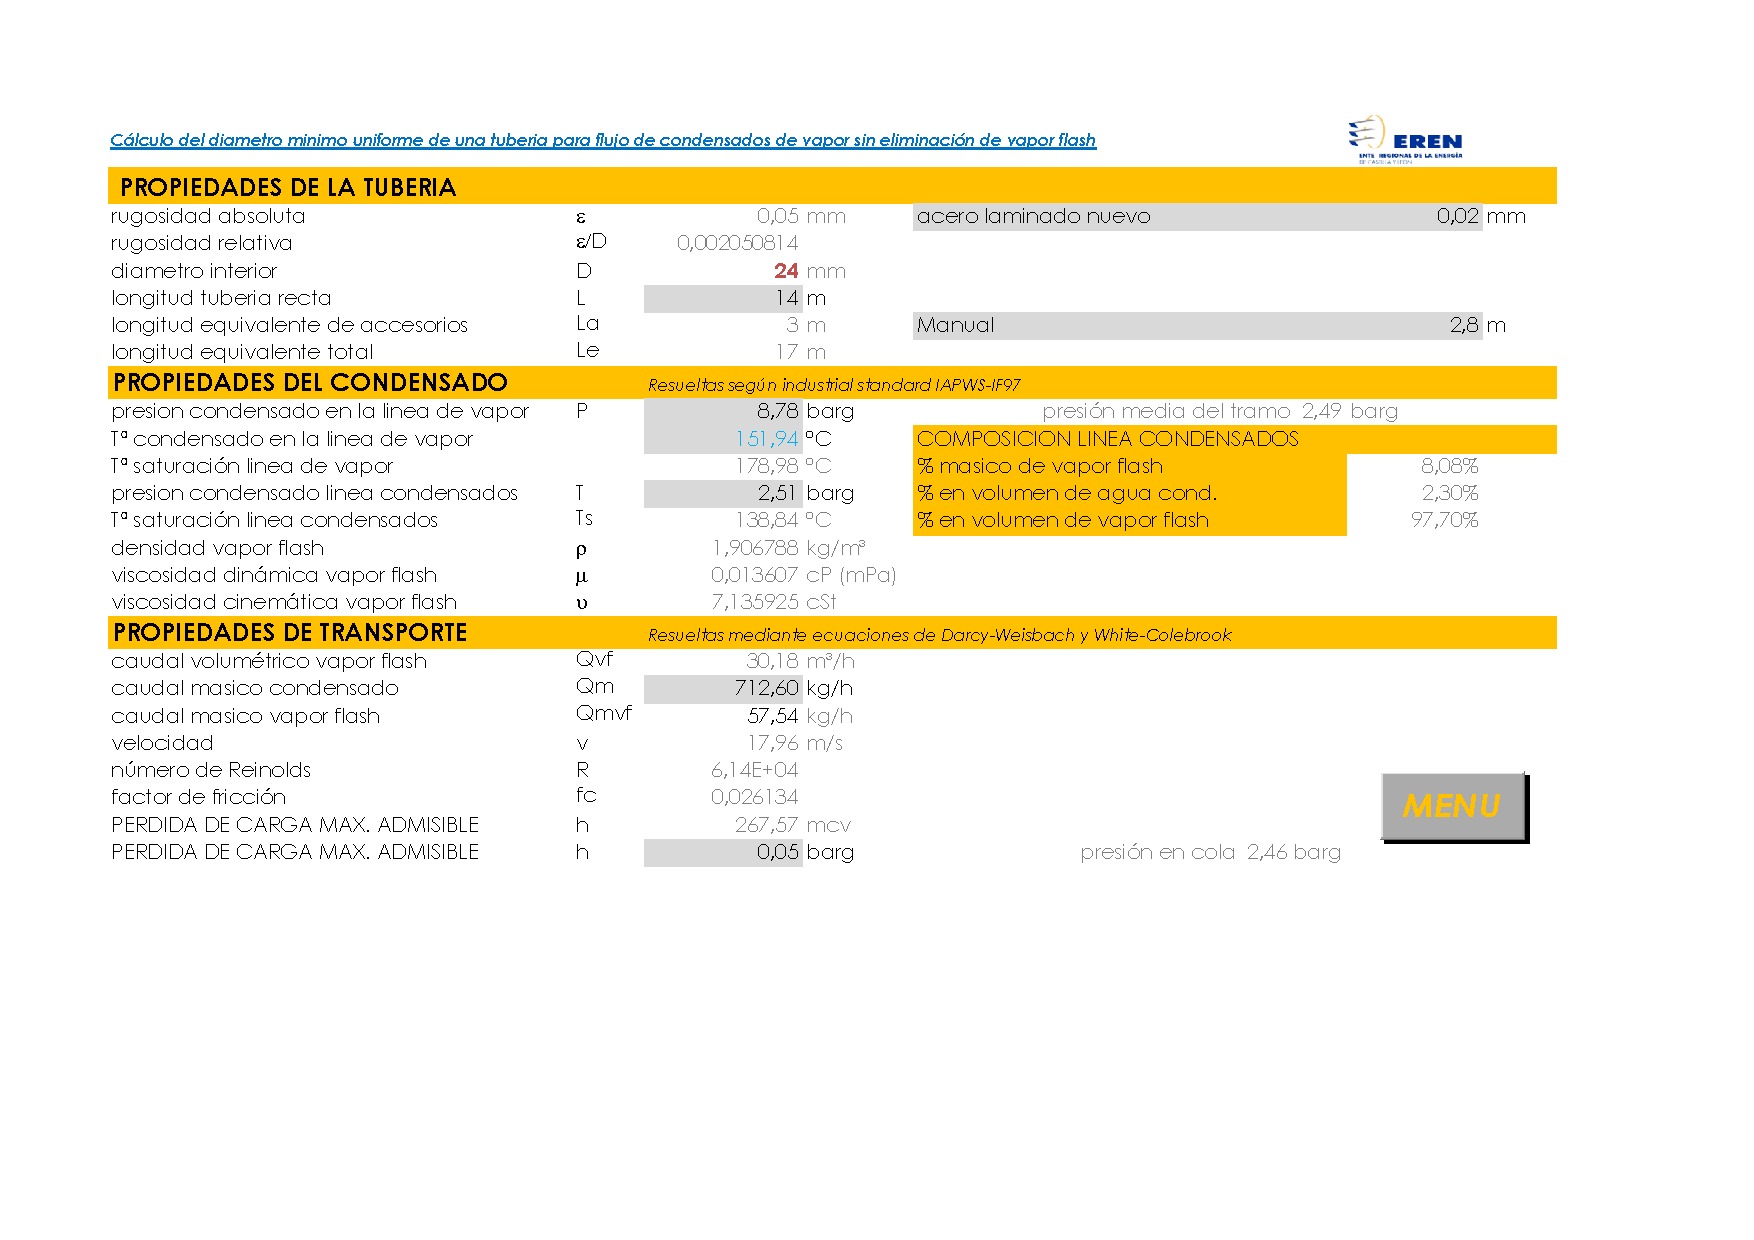
\includegraphics[trim={1cm 5cm 3cm 2cm}, clip = true,width=\textwidth]{Figuras/calculos_tramos/Condensados_TR6_T-C3.pdf}
	\caption{Hoja de cálculo del Tramo 6 de Condensados (T-C3). Fuente: Elaboración grupal.}
	\label{fig:anejo3-condensados-tr6}
\end{figure}

\begin{figure}[H]
	\centering
	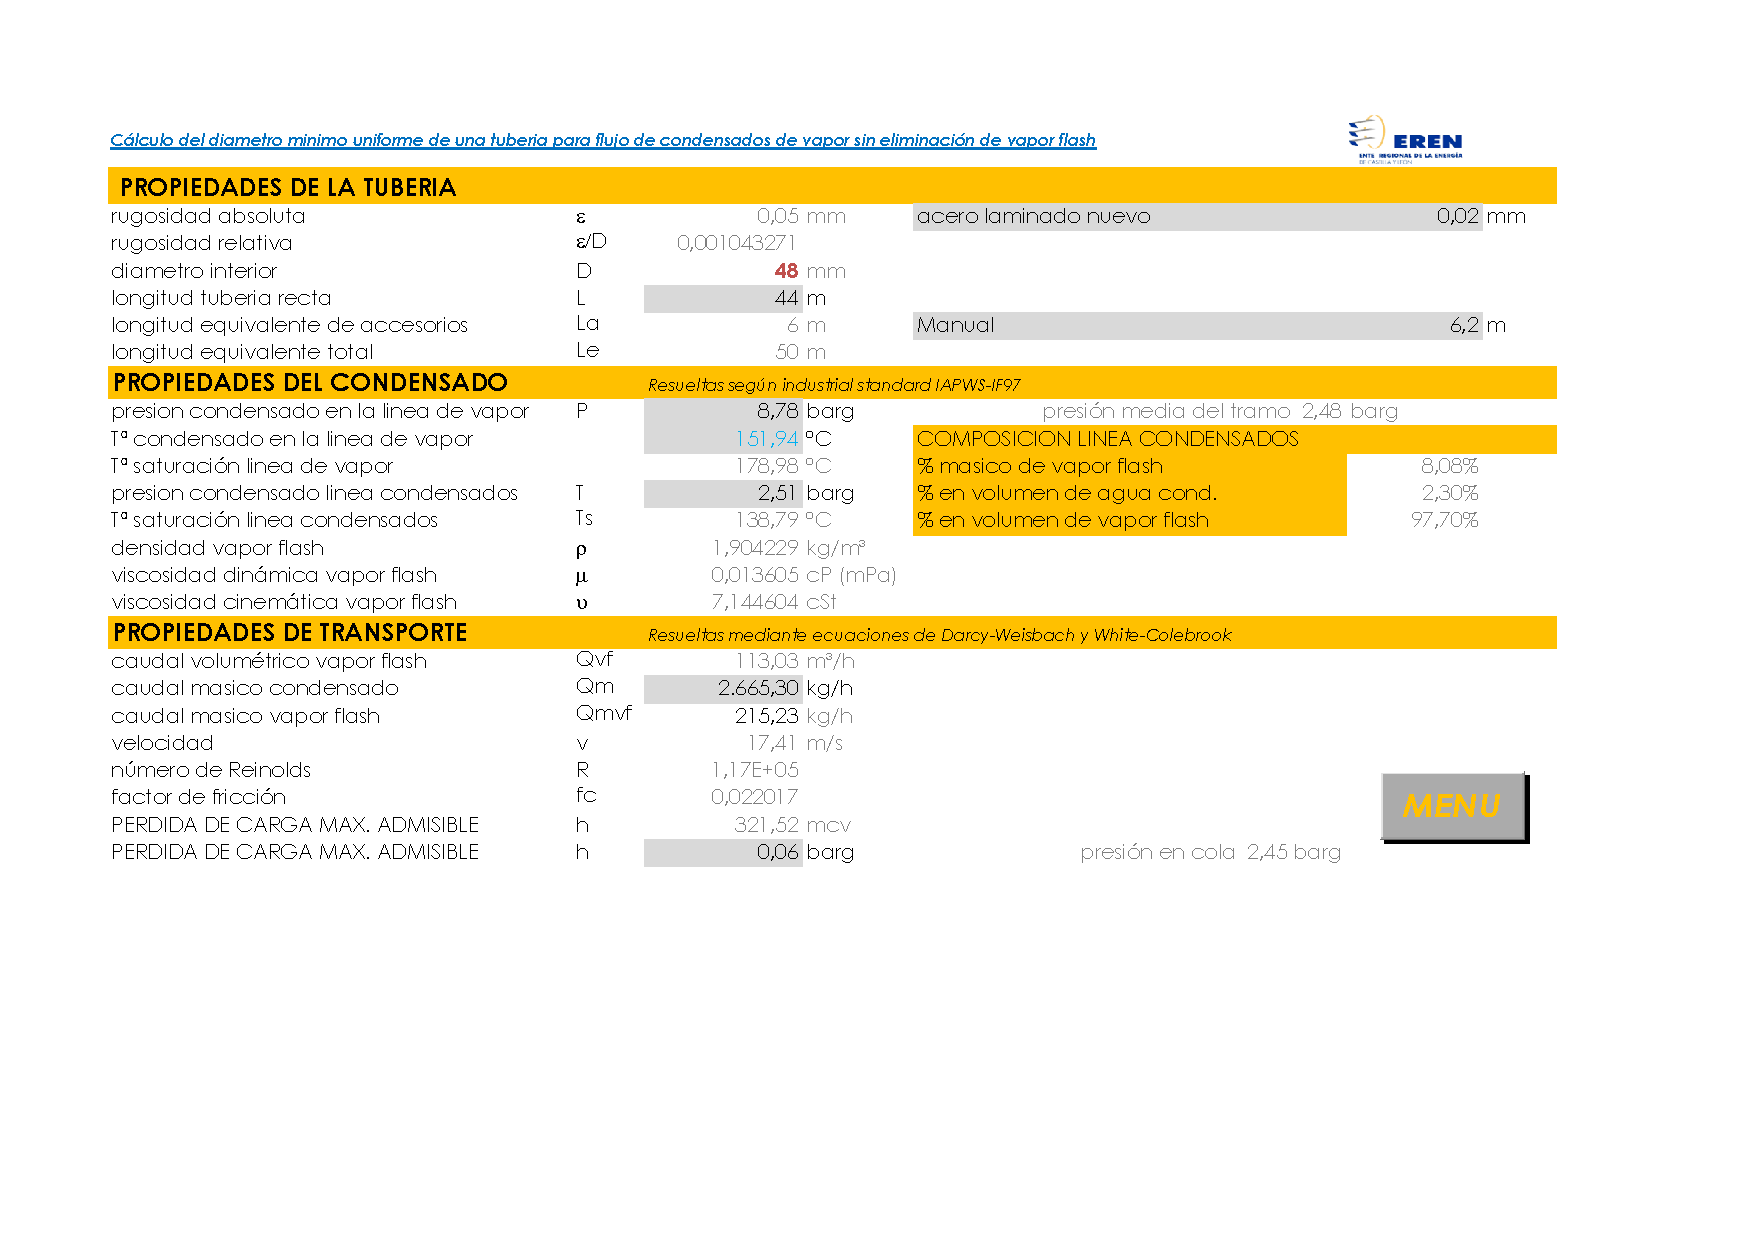
\includegraphics[trim={1cm 5cm 3cm 2cm}, clip = true,width=\textwidth]{Figuras/calculos_tramos/Condensados_TR7_T-C4.pdf}
	\caption{Hoja de cálculo del Tramo 7 de Condensados (T-C4). Fuente: Elaboración grupal.}
	\label{fig:anejo3-condensados-tr7}
\end{figure}

\end{document}
